\documentclass[letterpaper,12pt]{article}
\usepackage{changepage}
\addtolength{\skip\footins}{2pc plus 5pt}
\usepackage{geometry}
\usepackage{graphicx}
\usepackage{epsfig}
\usepackage{amsmath}
\usepackage{indentfirst}
\usepackage{float}
\usepackage{setspace}
\usepackage{amsfonts}
\usepackage[hidelinks]{hyperref} 
\usepackage{booktabs}
\usepackage{caption}
\usepackage{subfigure}
%\usepackage{times}
\usepackage{hyperref}
\usepackage{verbatim}
\usepackage{colortbl}
\usepackage{lscape}
\usepackage[affil-it]{authblk}
\usepackage{footnotebackref}
\usepackage[nodoi]{apacite}
\AtBeginDocument{\urlstyle{APACsame}}
\AtBeginDocument{\renewcommand{\APACrefYearMonthDay}[3]{\BBOP{#1}\BBCP}}
\usepackage{etoolbox}% http://ctan.org/pkg/etoolbox
\BeforeBeginEnvironment{tabular}{\footnotesize}% 

\geometry{left=2.54cm,right=2.54cm,top=2.54cm,bottom=2.54cm}

\setlength{\parindent}{2em}

\begin{document}
	
	\title{\textbf{Narrative Conservatism}\footnote{We are grateful for helpful comments from Bing Guo, Encarna Guillam\'on-Saor\'in, Paulo Maduro and seminar participants at the Universidad Carlos III de Madrid. We acknowledge financial contribution from the Spanish Ministry of Education and Science (ECO2016-77579 and PID2019-111143GB).}}

	\author{\normalsize \vspace{1cm}Juan Manuel Garc\'ia Lara}
	
	\author{Beatriz Garc\'ia Osma}
	
	\author{Fengzhi Zhu%
		\thanks{Corresponding author: Fengzhi Zhu. Department of Business Administration. Universidad Carlos III de Madrid. Calle Madrid 126, 28903 Getafe, Madrid (SPAIN). E-mail: fzhu@emp.uc3m.es}}
	
	\affil{Universidad Carlos III de Madrid}
	
	\date{\small This draft: \today}
	
	\maketitle
	
\thispagestyle{empty}
\begin{spacing}{1.5}

\begin{abstract}
	\begin{normalsize}
	\noindent
	We define narrative conservatism as narratives that reflect bad news in a more complete, news-consistent, and timely manner than good news. 
%	We proxy news by the market returns and measure completeness by the number of words, news-consistency by the marginal change of narrative tone in response to news, and timeliness by the reporting time lag between news release date and disclosure filing date. 
	Using 10-Q and 8-K filings from 1994 to 2019, we find that narrative disclosure is conservative. Narratives are asymmetrically lengthier, timelier, and show greater tone consistency in response to bad news than to good news. Firms report lengthier 10-Qs to clarify rather than obfuscate bad news, and provide more 8-Ks and 8-K items in response to bad news than to good news. We document greater narrative conservatism in the MD\&A section and in voluntary disclosure. We provide initial evidence that narrative conservatism is pervasive in firms with high conditional conservatism, intangible assets, R\&D expenses and proprietary costs. Finally, we find more narrative conservatism in settings where managers have strong incentives to disclose bad news, validating our empirical approach.\\
	\noindent\textbf{Keywords}: \textit{Narrative Disclosure; Narrative Conservatism; Conservatism; Tone; Timeliness; Textual Analysis}
	\end{normalsize}
\end{abstract}

\clearpage

\setcounter{page}{1}
\section{Introduction}
% Motivation
%Prior literature documents the existence of conditional and unconditional conservatism, which are measured by the recognized line items in financial statements. %recognition conservatism.\footnote{In this paper, we use the term ``recognition conservatism" to denote the union of conditional and unconditional conservatism, whose measurements are both derived from recognized line items in financial statements.} 
\noindent We define and provide evidence of narrative conservatism. We define narrative conservatism as \textit{narratives reflecting bad news in a more complete, news-consistent and timely manner than good news}. Our definition builds on the work of \citeA{basuConservatismPrincipleAsymmetric1997}, extending the notion of accounting conservatism to narratives. Narrative conservatism is of interest for at least two reasons. First, narrative disclosure takes up a dominant space in corporate filings.\footnote{For example, Apple Inc.'s 2019 Annual Report consists of 64 pages: 3 are numerical summaries of the financial statements, and 15 of other tables and figures. The remaining pages are narratives, including risk factors, management discussion and analysis (MD\&A), notes to financial statements (NFS), among other things. Over the past 20 years, the average number of pages in annual reports devoted to footnotes and MD\&A has quadrupled \cite{eyPointNowTime2012}.} Investors' perceptions of firm performance and their subsequent decision-making processes are influenced by narratives \cite{liTextualAnalysisCorporate2011}. Therefore, understanding the properties of narrative disclosure and their economic implications is essential for market participants and regulators. Second, studying narrative conservatism completes our understanding of accounting conservatism. Financial reporting consists both of recognition and disclosure, and thus, the extant knowledge of conditional and unconditional conservatism, which manifest through recognition, is a partial view of accounting conservatism. 

Consistent with this view, \citeA[p. 243]{kothariManagersWithholdBad2009} note that while prior research focuses on conservative \textit{recognition}, there is little evidence on conservative \textit{disclosure}. Guay and Verrecchia \citeyear[pp. 73-74]{guayConservativeDisclosure2018} call for more studies to focus on conservative reporting through narrative disclosure because ``a commitment to timely disclosure of bad news need not come exclusively through financial statement recognition.'' Despite these calls for further research, we know little about whether narrative disclosure is conservative, or whether and how narrative conservatism interacts with other forms of conservatism.

% Theory
\begin{comment}
	Prior studies distinguish between recognition and disclosure. Recognition is the depictions in numbers on the face of the financial statements, and disclosure is commonly viewed as the display in the notes and supporting schedules that accompany financial statements \cite{schipperRequiredDisclosuresFinancial2007}. The two formats of financial reporting are subject to different reporting requirements. The Financial Accounting Standards Board (FASB) explicitly specifies a set of recognition criteria while allowing for more flexibility in disclosure \cite{fasbStatementFinancialAccounting1984}. This flexibility paves the way for the supplementary role of disclosure---disclosing information that cannot be recognized due to the failure to meet one or more of the recognition criteria. The other explanatory role of disclosure is to provide detailed background information of recognized numbers in financial statements \cite[par. 7]{fasbStatementFinancialAccounting1984}. 
\end{comment}

An ample literature studies conditional and unconditional conservatism, concentrating on properties of income statement and balance sheet items. Conditional conservatism captures the asymmetric response of \textit{earnings} to positive and negative economic news \cite{basuConservatismPrincipleAsymmetric1997}, and unconditional conservatism manifests as a systematic understatement of \textit{net book value of assets} due to predetermined aspects of the accounting process \cite<e.g.,>[]{beaverConditionalUnconditionalConservatism2005}. We add to this literature by studying conservatism in narrative disclosure. 

To examine narrative conservatism, we build on fundamental properties of accounting information and their definitions. In particular, we focus on whether narratives respond to economic losses (bad news) in a more complete, news-consistent and timely manner than to economic gains (good news). Completeness implies that disclosure includes all necessary information for a user to understand the underlying economic event. News-consistency implies that disclosure agrees with the underlying economic event in content sentiment. Timeliness implies that disclosure is made \textit{in time} to be able to influence users' decisions. 

The existence of narrative conservatism is not clear ex-ante. Prior literature outlines managerial incentives both to disclose and withhold bad news \cite{healyInformationAsymmetryCorporate2001, kothariManagersWithholdBad2009, baoManagersDiscloseWithhold2019}. These incentives may also influence managers' decisions on whether, and to what extent, narrative disclosure responds to good and bad news asymmetrically. Overall, whether \textit{on average} firms respond to good and bad news asymmetrically in narrative disclosure remains an empirical question.

% Research Design
	% a. Proxies
To study whether narrative disclosure is conservative, we proxy completeness by the number of total words in corporate filings. We define news-consistency as the degree to which firms respond to good news with positive tone and to bad news with negative tone, and we measure it by the marginal change of narrative tone in response to news. The marginal change depicts how much narrative tone changes given one unit change in stock returns. 
%If narrative disclosure is conservative, the marginal change of tone in narrative disclosure should be greater in response to bad news than to good news. 
We evaluate timeliness by the reporting time lag between the news release date and the disclosure filing date. Overall, we posit that if narratives are conservative, they should have more words, greater marginal change of tone, and shorter reporting time lag in response to bad news than to good news. To measure news we follow \citeA{basuConservatismPrincipleAsymmetric1997} and use stock returns as our main proxy for news.

	% b. Corpora
We use two types of filings required by the U.S. Securities and Exchange Commission (SEC)---10-Q and 8-K filings---as our narrative disclosure corpora. 10-Qs provide a better setting to examine asymmetric completeness and asymmetric news-consistency, because they have more variation than 8-Ks in length and tone. 8-Ks are more appropriate than 10-Qs to study asymmetric timeliness for two reasons. First, 10-Qs are not as timely as 8-Ks because they are periodic filings with relatively fixed reporting schedules, so the reporting time lag of 10-Qs does not strictly proxy for narrative timeliness, whereas 8-Ks are used to disclose any material corporate events at any point of time, allowing for greater timeliness.\footnote{10-Qs are filled on a quarterly basis, and cannot be accelerated to reflect information in a timelier manner. For events that take place early (late) on in the quarter, the corresponding 10-Q would be relatively untimely (timely), irrespective of managerial intent to disclose bad news on a timely basis.}  Second, 10-Qs not only contain narrative disclosure but also financial statements,  whereas the 8-Ks contain mainly narrative disclosure.

% Data and Findings
	% a. Main results
We retrieve 10-Q and 8-K filings from the Electronic Data Gathering, Analysis, and Retrieval system (EDGAR) from 1993 to 2020.\footnote{Since the SEC adopted the rule of electronic submission for corporate filings in 1993, data coverage in the first year of EDGAR implementation is low \cite{gaoInformingMarketEffect2020}. We repeat our main analyses using data from 1994 onward, and our main results hold.} Next, we apply the financial sentiment word list developed by \citeA{loughranWhenLiabilityNot2011} (LM hereafter) to count the number of positive and negative words in each corporate filing. Finally, we construct NW as the natural logarithm of total words, TONE as the number of net positive words per thousand total words and TLAG as the number of days elapsed between the news release date and the SEC filing date. Our final 10-Q (8-K) sample consists of 91,606 (119,615) firm-quarter (firm-day) observations from 5,250 (8,261) unique firms. 

We report the following key findings. Our empirical results suggest that both 10-Q and 8-K filings have more words and greater marginal change of tone in response to bad news than to good news, consistent with narrative disclosure being conservative. In terms of reporting time lag, we find that 8-K filings are timelier in response to bad news than to good news while 10-Q filings do not respond to good and bad news asymmetrically. Overall, we interpret the results as evidence of narratives being conservative.

% b. Readability in 10-Q and number of items in 8-K
In addition, we investigate whether firms use lengthier reports in response to bad news to obfuscate bad news in 10-Qs. Using the Gunning fog index as the proxy for readability, we find that the incremental length in bad news disclosure contributes to higher readability, suggesting that firms tend to use shorter and less complex words in disclosing bad news compared to good news, and this trend is aligned with the SEC advocacy of plain English writing. Moreover, we check if the number of 8-K filings and items systematically varies in response to good and bad news. We find that firms are more likely to report more 8-K items and 8-K filings in response to bad news than to good news, consistent with firms responding to bad news with higher disclosure volume than good news.

% Additional Analyses
We perform five sets of additional analyses to explore other factors that affect narrative conservatism. First, to ensure that our results are not driven by boilerplate disclosure, we examine how narrative conservatism varies in MD\&A as compared with the notes to financial statements (NFS). We conjecture that narratives in MD\&A are more conservative because they contain less boilerplate than the NFS \cite{secFinancialReportingManual2019}. Our results are consistent with this prediction, confirming that our main findings are not driven by boilerplate. 

Second, we study whether narrative conservatism differs between voluntary and mandatory disclosure. Prior research suggests that managers have more freedom to determine the timing, content and rhetoric in voluntary disclosure than in mandatory disclosure \cite{segalAreManagersStrategic2016}. Thus, we expect voluntary disclosure to be more conservative than mandatory disclosure. Following \citeA{heMeasuringDisclosureUsing2020}, we measure voluntary and mandatory disclosure using 8-K filings that contain voluntary and mandatory 8-K items. Consistent with our expectation, narrative conservatism is mainly driven by voluntary disclosure. 

Third, we study if firms with higher intangible assets and research and development (R\&D) expenses are more conservative in narrative disclosure. The \citeA{fasbStatementFinancialAccounting1984} states that one essential role of narrative disclosure is to provide supplementary information that cannot be recognized because the underlying economic event fails to meet the recognition criteria. Because news regarding intangible assets is often less measurable and thus more likely to be disclosed rather than recognized, we expect firms with higher intangible assets to be more conservative in narrative disclosure. Also, because R\&D expenses cannot be capitalized, firms are more likely to disclose news regarding internally developed intangible assets via narratives. Therefore, we expect firms with higher R\&D expenses to be more conservative in narrative disclosure. Consistent with our expectation, we find that firms with high intangible assets and R\&D expenses are more conservative in terms of disclosure length.

Fourth, we study how narrative conservatism interacts with conditional conservatism and other firm characteristics. Following \citeA{khanEstimationEmpiricalProperties2009}, we measure conditional conservatism with C\_SCORE. We focus on four firm characteristics: firm size (SIZE), growth opportunities (MTB) and leverage (LEV) \cite{wattsConservatismAccountingPart2003, qiangEffectsContractingLitigation2007, khanEstimationEmpiricalProperties2009, laraEconomicDeterminantsConditional2009} and proprietary costs \cite{verrecchiaDiscretionaryDisclosure1983, liImpactsProductMarket2010}. Following \citeA{harrisAssociationCompetitionManagers1998}, we measure proprietary costs by Herfindahl index. We divide the full 10-Q sample into quintiles based on each firm characteristic and estimate our main model within each quintile. We find that firms in the high conditional conservatism quintiles also have high narrative conservatism, consistent with managers viewing narrative conservatism and conditional conservatism as complements. Also, we find that narrative conservatism increases with proprietary costs, consistent with competition inducing higher disclosure quantity and quality \cite{liImpactsProductMarket2010}. We do not find clear patterns of narrative conservatism along SIZE, MTB and LEV, consistent with C\_SCORE capturing conditional conservatism beyond its main determinants \cite{khanEstimationEmpiricalProperties2009}, and suggesting narrative conservatism may be driven by different determinants.

Fifth, we inspect whether and how managerial incentives affect narrative conservatism in three settings where managers have incentives to either disclose or withhold bad news. Prior studies document that when firms are undergoing a seasoned equity offering (SEO), managers have more incentives to withhold bad news \cite{teohEarningsManagementUnderperformance1998, langVoluntaryDisclosureEquity2000}. In contrast, when executives anticipate large stock option grants, managers have more incentives to disclose bad news \cite{yermackGoodTimingCEO1997, aboodyCEOStockOption2000}. We hypothesize and find evidence that the narrative disclosure of firms undergoing SEOs is less conservative, whereas that of firms issuing stock option grants is more conservative.

Moreover, we examine how litigation risk affects narrative conservatism. Prior literature provides mixed evidence on whether litigation induces managers to disclose or withhold bad news. One the one hand firms tend to disclose bad news to reduce the probability of being sued for late disclosure or to minimize the resolution costs in case that the litigation is inevitable \cite<e.g.,>{skinnerWhyFirmsVoluntarily1994,skinnerEarningsDisclosuresStockholder1997}. On the other hand, firms withhold bad news given that bad news disclosure can trigger litigation \cite<e.g.,>{francisShareholderLitigationCorporate1994}. We find that firms with high litigation risk are less conservative compared to firms with low litigation risk in terms of disclosure completeness and news-consistency. Our finding echos Rogers and Van Buskirk's \citeyear{rogersShareholderLitigationChanges2009} that firms reduce disclosure to avoid litigation, and provides indirect evidence in line with  \citeA{francisShareholderLitigationCorporate1994}, that bad news disclosure may trigger litigation.

Finally, in untabulated robustness checks, we find that our evidence of is robust to (a) employing an alternative tone measure using the positive and negative word list from the Harvard General Inquiry dictionary \cite{loughranTextualAnalysisAccounting2016}, (b) including controls for conditional conservatism and managerial incentives, (c) excluding 8-K items on results of operations that contain quarterly or annual financial statements \cite{segalAreManagersStrategic2016}, (d) using an alternative 8-K reporting time lag definition \cite{carterRelevanceForm8K1999, niessnerStrategicDisclosureTiming2015, chapmanInformationOverloadDisclosure2019}, (e) excluding a priori bad news 8-K items \cite{segalAreManagersStrategic2016}, and (f) annual regressions in more than two thirds of the years from 1995 to 2020.

% [Contribution]
Our study contributes to the accounting literature in three aspects. First, we document the existence of narrative conservatism. Prior studies focus on two forms of conservatism---the asymmetric earnings response to good and bad news and the understatement of net asset values \cite{basuConservatismPrincipleAsymmetric1997, ballEarningsQualityUK2005, beaverConditionalUnconditionalConservatism2005}. We extend the notion of conservatism to the asymmetric narrative response to good and bad news. 
% Second, we add to the literature on the interaction between recognition and disclosure \cite{aboodyRecognitionDisclosureOil1996, barthMarketEffectsRecognition2003, schipperRequiredDisclosuresFinancial2007}. We find that firms with high conditional conservatism tend to be more conservative in narratives as well, suggesting that recognition and disclosure are complements in financial reporting. 
Second, we provide novel evidence to the debate regarding whether managers withhold bad news. Prior research uses a wide variety of disclosure proxies to study managers' tendency to disclose or withhold bad news \cite{kasznikWarnNotWarn1995, kothariManagersWithholdBad2009, baoManagersDiscloseWithhold2019}. We use the textual properties of SEC filings as novel proxies for disclosure, and our results support the idea that firms on average disclose bad news in a more complete, news-consistent and timely fashion. Third, we relate to the broader literature on the informativeness of SEC filings. A stream of literature studies the market reactions to 8-Ks \cite{carterRelevanceForm8K1999, pinskerHasFirmsForm2006, lermanNewForm8K2010} and 10-K/Qs \cite{alfordExtensionsViolationsStatutory1994, liAnnualReportReadability2008, liInformationContentForwardLooking2010}. We add to this literature by studying the behavior of corporate narrative disclosure in response to good and bad news, using the market movements as an indicator of the underlying news.

The rest of the study is as follows. Section 2 reviews prior literature and develops our main hypotheses. Section 3 outlines the empirical design and the data selection process. Section 4 presents the main results. Section 5 reports the additional analyses and Section 6 concludes.

\section{Theoretical Framework}
\subsection{Recognition and Disclosure}\label{sec2.1}
% What are recognition and disclosure?
\noindent A stream of literature studies the distinctions between recognition and disclosure and their effects \cite{aboodyRecognitionDisclosureOil1996, barthMarketEffectsRecognition2003}. \citeA[p. 301]{schipperRequiredDisclosuresFinancial2007} defines recognition as ``depictions in numbers with captions on the face of the financial statements," and disclosure as ``display in the notes and supporting schedules that accompany financial statements."\footnote{Statement of Financial Accounting Concepts No. 5---\textit{Recognition and Measurement in Financial Statements of Business Enterprises} formally defines \textit{recognition} as ``the process of formally recording or incorporating an item into the financial statements of an entity as an asset, liability, revenue, expense, or the like. Recognition includes depiction of an item in both words and numbers, with the amount included in the totals of the financial statements." \cite[par. 6]{fasbStatementFinancialAccounting1984} but does not define \textit{disclosure}. Due to the absence of a conceptual definition of disclosure, prior literature on disclosure commonly interpret disclosure as any display that is not in numbers. However, this interpretation may partially overlap with the FASB definition of recognition, which states that recognition also includes words. As \citeA[p. 302]{schipperRequiredDisclosuresFinancial2007} notes: ``both in analytical modeling and in developing financial reporting concepts, it is difficult to distinguish between recognized and disclosed information."} We follow \citeA{schipperRequiredDisclosuresFinancial2007} and use the term narrative (or narrative disclosure) to denote textual disclosures presented in SEC filings, including notes to financial statements, supplementary information, and other means of financial reporting such as MD\&As.\footnote{Because narrative disclosure in different sections may employ boilerplate to different extent, in additional analyses we examine narrative conservatism in the MD\&A and in the notes to financial statements separately.}

% What are the recognition criteria and the role of narrative?
Disclosure and recognition are subject to different reporting requirements. For an economic event to be recognized in financial statements, a set of recognition criteria needs to be satisfied \cite{fasbStatementFinancialAccounting1984}. First, the item must meet the definition of an element of financial statements (definition criterion). Second, the item must have a relevant attribute measurable with sufficient reliability (measurability criterion). Third, the information about the item must be capable of making a difference in user decisions (relevance criterion). Fourth, the information must be representationally faithful, verifiable, and neutral (reliability criterion). 

In contrast, disclosure is more flexible because it can be deployed to disclose information that fails to meet certain recognition criteria \cite[par. 7b]{fasbStatementFinancialAccounting1984}. Narrative disclosure plays an essential role in financial reporting, as \citeA[par. 7, CON5-7]{fasbStatementFinancialAccounting1984} states:
\begin{adjustwidth}{1cm}{1cm}
\begin{singlespace}
	\textit{Although financial statements have essentially the same objectives as financial reporting, some useful information is better provided by financial statements and some is better provided, or can only be provided, by notes to financial statements or by supplementary information or other means of financial reporting.}
\end{singlespace}
\end{adjustwidth}

Narrative disclosure serves two key roles. First, narratives can be \textit{supplementary} to recognition, conveying information that cannot be recognized because it fails to meet the recognition criteria. With respect to good news, because good news recognition requires a higher standard of verification, firms may convey good news via disclosure rather than recognition. For instance, under U.S. General Accepted Accounting Principles (US GAAP), long-lived tangible and intangible assets cannot be revaluated upwards. When the market price of the firms' long-lived tangible and intangible assets goes up, the firms cannot recognize the gain, but they may discuss the appreciation in other filings. With respect to bad news, despite lower verification criteria, bad news may still not be fully recognized. For example, although firms could create a provision for the expected future payments from a potential lawsuit, they cannot recognize the associated reputation losses since it is extremely difficult to obtain a reliable estimate that can be verified subsequently. However, firms may discuss the likelihood and the expected reputation impact of entering into a lawsuit in the risk factors or the MD\&A section of the SEC filings. Another example would be internally developed intangible assets, which cannot be capitalized, and thus, cannot be impaired when bad news arrives. However, firms may discuss the impact of news associated with these intangible assets in other filings. In sum, firms may use narrative disclosure to inform investors about the immeasurable, and thus non-recognizable impact of various corporate events to fulfil their obligation of providing relevant financial information to investors.\footnote{Rule 10b-5 of the Securities Exchange Act of 1934 states that it shall be unlawful ``to omit to state a material fact necessary in order to make the statements made ... not misleading."} 

Second, narratives can be \textit{complementary} to recognition. Complementary narratives are used to explain or provide essential descriptive information to the line items included in the firm financial statements. For example, for long-term obligations, narratives describe the due amounts, the interest rate and restrictions imposed by covenants, etc. For inventory, narratives state the measurement method used. In case of an impairment, the narrative may explain the circumstances surrounding it. For sales, narratives provide revenue recognition policies \cite[footnote 4, CON5-7]{fasbStatementFinancialAccounting1984}. In sum, firms may use narrative disclosure to complement the line items recognized in the financial statements, thereby enhancing users' understanding about the underlying economic events.

\begin{comment}
	\citeA[footnote 4, CON5-7]{fasbStatementFinancialAccounting1984} gives several examples on the complementary role of notes to financial statements:
	
	\begin{adjustwidth}{1cm}{1cm}
	\begin{singlespace}
	\indent \textit{For example, notes provide essential descriptive information for long-term obligations, including when amounts are due, what interest they bear, and whether important restrictions are imposed by related covenants. For inventory, the notes provide information on the measurement method used---FIFO cost, LIFO cost, current market value, etc. For an estimated litigation liability, an extended discussion of the circumstances, counsel's opinions, and the basis for management's judgment may all be provided in the notes. For sales, useful information about revenue recognition policies may appear only in the notes (FASB Statement No. 47, Disclosure of Long-Term Obligations; ARB No. 43, Chapter 4, ``Inventory Pricing", statement 8; FASB Statement No. 5, Accounting for Contingencies, par. 10; and APB Statement 4, par. 199)}.
	\end{singlespace}
	\end{adjustwidth}
\end{comment}

\subsection{Definition of Narrative Conservatism}\label{sec2.2}
% What are conditional and unconditional conservatism?
\noindent Prior work documents two main manifestations of accounting conservatism: conditional and unconditional conservatism \cite{beaverConditionalUnconditionalConservatism2005}. Conditional conservatism manifests as ``accountants' tendency to require a higher degree of verification to recognize good news as gains than to recognize bad news as losses" \cite[p. 7]{basuConservatismPrincipleAsymmetric1997},\footnote{\citeA{basuConservatismPrincipleAsymmetric1997} does not use the terms conditional or unconditional conservatism. Here we quote \citeA{basuConservatismPrincipleAsymmetric1997} only to describe the manifestation of the two forms of conservatism, which are now labeled as conditional and unconditional conservatism.} and is typically measured by the asymmetric response of earnings to positive and negative stock returns. Examples of conditional conservatism under US GAAP include impairment/revaluation accounting for long-lived tangible and intangible assets, which mandates writing down the value of an asset by any losses incurred, but not writing up its value by the difference between market price and its carrying amount. Another example of conditional conservatism is lower of cost or market accounting for inventory under US GAAP or lower of cost or net realizable value accounting under International Financial Reporting Standards (IFRS). 

With respect to unconditional conservatism, it manifests as ``accountants' preference for accounting methods that lead to lower reported values for shareholders' equity" \cite[p. 8]{basuConservatismPrincipleAsymmetric1997}. Examples of unconditional conservatism include the immediate expensing, rather than capitalizing of research and development (R\&D) costs, and the use of accelerated depreciation for property, plant and equipment \cite{beaverConditionalUnconditionalConservatism2005}. 

% What is narrative conservatism and why focus on the three constructs?
Compared to the extant literature on conditional and unconditional conservatism in recognition, little work has been done on conservatism in disclosure. One notable exception is Guay and Verrecchia \citeyear{guayConservativeDisclosure2018} that study firms' commitment to disclose bad realizations of economic events in an analytical model. Guay and Verrecchia \citeyear[p. 73]{guayConservativeDisclosure2018} interpret a commitment to conservative reporting to include ``not only reported earnings, but, more broadly, any mechanism that commits managers to disclose, such as required footnotes and explanations in corporate filings."
\begin{comment}
	As \citeA[p. 243]{kothariManagersWithholdBad2009} state:
	\begin{adjustwidth}{1cm}{1cm}
	\begin{singlespace}
	\textit{Considerable research examines conservative} recognition \textit{in accounting in the United States and internationally (Basu [1997], Ball, Kothari, and Robin [2000], McNichols [1988]). However, there is little systematic evidence to suggest conservatism in firms’} disclosure \textit{practices, with the notable exception of disclosure of bad news to mitigate litigation risk.}
	\end{singlespace}
	\end{adjustwidth}
	In a recent analytical work, \citeA[pp. 73-74]{guayConservativeDisclosure2018} have expressed similar opinions:
	\begin{adjustwidth}{1cm}{1cm}
	\begin{singlespace}
	\textit{By way of an analogy, 20 years ago, much of the accounting literature on transparent financial disclosure emphasized constructs such as earnings timeliness, high-quality accruals, and asset/liability recognition. Today, scholars study a plethora of additional financial disclosure mechanisms, including management forecasts, conference calls, management discussion and analysis (MD\&A) disclosure, press releases, and social media outlets. A commitment to timely disclosure of bad news need not come exclusively through financial statement recognition, and we believe that a broader view of conservative disclosure will offer new paths forward for a literature that has struggled to develop theories to explain the efficiency of timely asymmetric earnings numbers. We encourage researchers to pursue these avenues to better understand how the very large literature on conservative financial reporting integrates with the equally large literature on corporate disclosure.}
	\end{singlespace}
	\end{adjustwidth}
\end{comment}


The model in Guay and Verrecchia \citeyear{guayConservativeDisclosure2018} focuses on the timeliness dimension of recognition and disclosure. We build on their analytical work and extend the notion of narrative conservatism to three dimensions of disclosure. Specifically, we define narrative conservatism as \textit{narratives reflecting bad news in a more complete, news-consistent and timely manner than good news}. Narratives can be conservative or not along each of these dimensions. We explain these dimensions next.

\subsubsection{Asymmetric completeness with respect to good and bad news}

\noindent Financial information is of higher quality when it is \textit{complete}. Complete disclosure must include all necessary information for a user to understand the underlying economic event. Extant theoretical studies establish that managerial commitment to complete disclosure of news, good or bad, reduces information asymmetry and improves market efficiency \cite{glostenBidAskTransaction1985, diamondOptimalReleaseInformation1985, diamondDisclosureLiquidityCost1991, baimanRelationCapitalMarkets1996}. Empirically, using German data, \citeA{leuzEconomicConsequencesIncreased2000} show that firms' information asymmetry is reduced, and cost of capital is lowered after switching to the international reporting regime which requires an increased level of disclosure. \citeA{leuzDisclosureCostCapital2009} find that firms respond to the adverse shock of Enron scandal by increasing their disclosure level through lengthier 10-K filings, thereby reducing their cost of capital. 

Against this backdrop, we propose completeness as an essential attribute of disclosure. Narratives are conservative if they are more complete when disclosing bad news than when disclosing good news, i.e., narrative disclosure is conservative if it is asymmetrically complete in response to good versus bad news. 

In practice, firms may disclose good news in a more complete manner than bad news. \citeA{kothariEffectDisclosuresManagement2009} find that favorable disclosure decreases cost of capital while unfavorable disclosure increases it significantly. This penalization of bad news disclosure from frictional capital markets may induce managers to disclose good news and withhold bad news, leading to asymmetric completeness in narrative disclosure but in the opposite direction of narrative conservatism. \citeA{teohEarningsManagementUnderperformance1998} and \citeA{langVoluntaryDisclosureEquity2000} provide supporting evidence to this argument by documenting that firms issuing equity tend to disclose good news and withhold bad news. \citeA{rogersShareholderLitigationChanges2009} find that firms reduce the frequency and amount of disclosure post-litigation, suggesting that firms become more likely to withhold bad news for which they may later be held legally accountable. 

In contrast to this work, other studies document that managers have incentives to disclose bad news in a more complete manner than good news. \citeA{skinnerWhyFirmsVoluntarily1994, skinnerEarningsDisclosuresStockholder1997} finds that firms preempt negative earnings surprises with voluntary bad news disclosure to avoid being sued, or to minimize the costs of resolving any litigation that follows the disclosure of bad news. In line with this argument, \citeA{fieldDoesDisclosureDeter2005} find that disclosure of bad news deters certain types of litigation. 

In sum, it is unclear whether narratives are conservative in terms of disclosure completeness ex-ante. If narrative disclosure is conservative, firms should respond to bad news in a more complete manner than to good news. We formulate our first hypothesis as follows:

\begin{quote}\label{hyp:h1}
\textit{\textbf{H1:} Narrative disclosure is completer in response to bad news than to good news.}
\end{quote}

\subsubsection{Asymmetric news-consistency with respect to good and bad news}

\noindent We introduce the concept of \textit{news-consistency} to assess \textit{how} information is provided, and we interpret it as the degree to which firms use positive tone in narrative disclosure in response to good news and negative tone in response to bad news. %As the old adage goes, ``It's not what you say; it's how you say it.'' 
Tone influences how information is perceived or processed, and thus it can be employed both to inform or mislead. \citeA{davisNumbersMeasuringInformation2012} document that increases in tone optimism in earnings press releases are positively associated with immediate stock price response. Using a naïve Bayesian machine learning approach, \citeA{liInformationContentForwardLooking2010} finds that the average tone of forward looking statements in MD\&As is positively correlated with future earnings. Thus, news-consistency refers to whether and to what extent disclosure tone aligns with the real impact of the underlying economic event, and it is likely to affect market reactions to the disclosure. 

% Narrative conservatism implies that firms emphasize bad news more than good news using narrative tone. However, the Conceptual Framework requires financial information to be \textit{neutral}, i.e., ``not slanted, weighted, emphasized, deemphasized, or otherwise manipulated to increase the probability that financial information will be received favorably or unfavorably by users.'' \citeA[QC14]{fasbConceptualFrameworkFinancial2018} We note that narrative conservatism conflicts with the neutrality principle. 

Therefore, we propose news-consistency as a second critical attribute of disclosure. Firms may deploy a uniformly positive tone in both good and bad news disclosure, resulting in higher news-consistency in good news disclosure. For example, \citeA{huangToneManagement2014} document that firms strategically engage in upward tone management to boost market perception of firm performance. Based on their findings, when managers have incentives to emphasize the economic impact of good news, they may disclose bad news using positive tone, thereby creating higher news-consistency in response to good relative to bad news. Nevertheless, to avoid litigation risk, managers may deploy a uniformly negative tone in both good and bad news disclosure, resulting in higher news-consistency in response to bad news disclosure relative to good news. \citeA[p. 2179]{rogersDisclosureToneShareholder2011} suggest that ``managers can reduce litigation risk by dampening the tone of their earnings announcements either by decreasing their use of positive language or by tempering their optimism with statements that are less favorable.'' Consistent with litigation risk constraining the use of optimistic tone in disclosure, \citeA{tama-sweetManagersAlterTone2009} finds that managers increase optimistic tone prior to option exercises when litigation risk is low, but decrease optimistic tone prior to option exercises when litigation risk is high. Based on the mixed prior evidence, whether narrative disclosure is conservative in terms of news-consistency is unclear ex-ante. If narratives are conservative, firms should respond to bad news in a more news-consistent manner than to good news. We formulate our second hypothesis as follows:

\begin{quote}\label{hyp:h2}
\textit{\textbf{H2:} Narrative disclosure is more news-consistent in response to bad news than to good news.}
\end{quote}

\subsubsection{Asymmetric timeliness with respect to good and bad news}

\noindent Financial information is of higher quality if it is \textit{timely}. Disclosure should be made \textit{in time} to influence users' decisions. Managers have discretion over the timing of disclosure \cite<e.g.,>{chapmanInformationOverloadDisclosure2019}, and this timing influences market reaction to disclosure. \citeA{alfordExtensionsViolationsStatutory1994} find that the market reacts negatively to delays in the filing of 10-Ks. As a final attribute of disclosure, we focus on timeliness.

Commonly, managers disclose good news in a timely manner, while the evidence on the timeliness of bad news disclosure is mixed. Several studies document that managers tend to delay bad news disclosure. For instance, \citeA{chambersTimelinessReportingStock1984} find that firms accelerate good news disclosure while delaying bad news disclosure, and that investors interpret the failure to report on time as a forecast of bad news. \citeA{segalAreManagersStrategic2016} find that managers release bad news after trading hours and on the last trading day of the week to exploit investor inattention and minimize the negative impact on stock price. This strategic timing of bad news disclosure is also prevalent in private firms without stock price motivations \cite{brockbankStrategicTiming8K2018} and is associated with benefits in insider sales \cite{niessnerStrategicDisclosureTiming2015}. \citeA{baginskiCareerConcernsAffect2018} document that firms' delayed disclosure of bad news is positively associated with managerial career concerns. However, other studies document that firms disclose bad news in a timely manner. \citeA{skinnerWhyFirmsVoluntarily1994} argues that managers may face reputational costs if they fail to disclose bad news in a timely manner prior to a negative earnings surprise. Using a continuous-time disclosure model, \citeA{marinovicNoNewsGood2016} show that litigation risk not only induces timely bad news disclosure, but also suppresses good news disclosure since the market interprets silence as good news and firms can communicate good news without actually disclosing it, lowering proprietary costs. \citeA{yermackGoodTimingCEO1997} and \citeA{aboodyCEOStockOption2000} find that managers prompt bad news disclosure prior to stock option grant dates to lower option strike prices. 

In sum, it is unclear whether narratives are conservative in terms of disclosure timeliness ex-ante. If narrative disclosure is conservative, firms should respond to bad news in a timelier manner than to good news. We formulate our third hypothesis as follows:

\begin{quote}\label{hyp:h3}
\textit{\textbf{H3:} Narrative disclosure is timelier in response to bad news than to good news.}
\end{quote}

\begin{comment}
\subsection{Conditional, Unconditional and Narrative Conservatism: Usefulness}
% conservatism role: stewardship or neutrality
The controversy regarding whether conservatism is a desirable property that enhances the usefulness of financial reporting persists. Traditionally, the usefulness of accounting information can be assessed in terms of how well it serves each of the two objectives of accounting---valuation and stewardship \cite{cascinoUsefulnessFinancialAccounting2017}. The valuation objective is to ``provide financial information about the reporting entity that is useful to existing and potential investors, lenders, and other creditors in making decisions about providing resources to the entity \cite[OB2]{fasbConceptualFrameworkFinancial2018b}". For financial information to be useful for valuation objective, it must be relevant and faithfully represent what it purports to represent. Faithful representation further requires neutrality, which means that a depiction must be ``not slanted, weighted, emphasized, deemphasized, or otherwise manipulated to increase the probability that financial information will be received favorably or unfavorably by users". The stewardship objective is to assess ``how efficiently and effectively the entity's management and governing board have discharged their responsibilities to use the entity's economic resources \cite[OB4]{fasbConceptualFrameworkFinancial2018b}". Although not separately stated in the Conceptual Framework as one primary purpose of financial reporting, the stewardship role of accounting dates back several millennia and has been one of the main reasons for the existence of accounting \cite{lennardStewardshipObjectivesFinancial2007, murphyDiscoursesSurroundingEvolution2013, pelgerPracticesStandardsettingAnalysis2016}. On the one hand, conservatism contradicts the valuation role of accounting by introducing downward bias in financial reporting and thus weakening its ability to faithfully represent firm performance. For example, unconditional conservatism encourages firms to anticipate and recognize losses before their realization, resulting in a systematic downward bias in asset valuation \cite<e.g.,>[]{wattsPositiveAccountingTheory1986}. Conditional conservatism requires higher verification for good news to be recognized than bad news, leading to asymmetric timeliness in gain and loss recognition in earnings \cite<e.g.,>[]{basuConservatismPrincipleAsymmetric1997}. On the other hand, conditional conservatism enhances the stewardship role of accounting by improving contract efficiency. For example, in compensation contracting conditional conservatism limits managers' ability to overstate earnings and thus maximizing personal wealth at the expense of other claimholders \cite<e.g.,>[]{wattsConservatismAccountingPart2003}.

Aligned with the prior literature on the usefulness of conservatism, we argue that more complete, news-consistent and timely disclosure of bad news relative to good news enhances contract efficiency [specific hypotheses to be developed]. However, we do not make claims about the valuation role of narrative conservatism.

\end{comment}

\section{Research Design}
\subsection{Proxies for Textual Properties and News} \label{sec3.1}
\noindent We use length, marginal change of tone, and reporting time lag as proxies for disclosure completeness, news-consistency, and timeliness respectively. Specifically, we measure disclosure completeness by the total number of words of SEC filings. Complete disclosure should include ``all information necessary for a user to understand the phenomenon being depicted, including all necessary descriptions and explanations" \cite[QC12]{fasbConceptualFrameworkFinancial2018}. Hence, more complete disclosure should be lengthier, to allow managers to elaborate on detailed explanations  \cite{leuzDisclosureCostCapital2009}.\footnote{We use number of words instead of number of pages, which is used in \citeA{leuzDisclosureCostCapital2009}, as the proxy for disclosure completeness for two reasons. First, for pure texts, these two measures are almost equivalent, or at least are monotonic transformations of each other, given a roughly constant number of words per page. Second, for financial reports with graphs and tables, the number of words is a more precise measure for narrative disclosure, because it counts the length of narratives only. However, the number of pages may be enlarged mechanically by graphs, tables, and even space lines embedded in the tables, which are not the focus of this study.} We are aware of a strand of literature suggesting that narrative disclosure is less informative when it is less readable \cite{liAnnualReportReadability2008, loEarningsManagementAnnual2017, loughranMeasuringReadabilityFinancial2014}, and because lengthier documents are often less readable, it may appear counter-intuitive to proxy completeness with document length. We provide two explanations for this measurement. First, lower readability may result from the fact that bad news is inherently more complex and therefore needs more explanations \cite{bloomfieldDiscussionAnnualReport2008}, and there is incremental information content embedded in complex narratives \cite{busheeLinguisticComplexityFirm2018}. Therefore, lower readability does not necessarily imply lower narrative disclosure quality. Second, although somewhat correlated, length and readability are essentially two different constructs. Texts can be long or short, readable or illegible independently. %Specifically, in measuring information completeness, the document length is an appropriate construct because ``including all necessary descriptions and explanations" \cite[QC12]{fasbConceptualFrameworkFinancial2018} inevitably increases the document length. 

Given the arguments above, if narrative disclosure is conservative, we expect it to have more words in response to bad news than to good news. In our additional tests, we address the above concerns by directly testing whether narrative disclosure responds asymmetrically to good and bad news in terms of readability.

We proxy the sentiment in narrative disclosure by linguistic tone and measure the degree of news-consistency by the marginal change of tone in response to increase (good news) or decrease (bad news) in stock market returns. News-consistency requires the marginal change to be positive, i.e., tone is positive in response to good news, and negative in response to bad news. Furthermore, if narrative tone is asymmetrically news-consistent, it implies greater marginal change of tone in response to bad news than to good news. That is, if narrative disclosure is conservative, the change in narrative tone should be more negative in response to bad news than it should be positive in response to good news, given the same magnitude of news. Irrespective of the nature of news, under narrative conservatism, either bad news is emphasized or good news is attenuated, or both.\footnote{We provide the following numerical example to illustrate the concept of marginal change of tone. Suppose a 1\% increase (good news) versus a 1\% decrease (bad news) in stock return, which should move tone upwards and downwards, respectively, by 1\% if the response of narrative tone is neutral, i.e., tone responds equally  to good and bad news. However, in the presence of narrative conservatism, three situations may happen: (1) bad news emphasis: in response to bad news, tone decrease by 1.2\% and in response to good news, tone increase by 1\%; (2) good news attenuation: in response to bad news, tone decrease by 1\% and in response to good news, tone increase by 0.8\%; (3) a mix of both: in response to bad news, tone decrease by 1.2\% and in response to good news, tone increase by 0.8\%. In all cases, the marginal change of tone in response to bad news is greater in magnitude than that in response to good news. Therefore, under narrative conservatism, the marginal change of tone in narrative disclosure is greater in response to bad news than to good news.} 

We measure timeliness by the reporting time lag, defined as the number of days elapsed between the news release date and the filing date of the studied disclosure.\footnote{A concern with TLAG is that the length of reporting time lag may not be fully controlled by managers, and thus cannot accurately capture discretionary reporting timeliness. Prior auditing literature suggests that auditor characteristics contributes to unexpected audit report lag \cite{knechelAdditionalEvidenceAudit2001, bamberAuditStructureOther1993}, which leads to filing delay in audited financial reports. However, because audit for quarterly filings is not mandated by law, and due to high auditing costs and time constraints, most 10-Q filings are not audited. 8-K filings are not required to be audited to our knowledge.} Specifically, in the 10-Q sample, it is calculated as the number of days between the quarter-end and the filing date. In the 8-K sample, it is the number of days between the news day, i.e., the nearest date around an 8-K reporting period date when there is a large change (as defined in \hyperref[sec3.3.2]{Section 3.3.2}) in stock daily returns, and the filing date of the corresponding 8-K.\footnote{Alternatively, we calculate the 8-K reporting time lag as the number of days between the 8-K reporting period date and the 8-K filing date \cite{carterRelevanceForm8K1999, niessnerStrategicDisclosureTiming2015, chapmanInformationOverloadDisclosure2019}. Our results (untabulated) remain unchanged.} The shorter the lag, the timelier the narrative disclosure. If narrative disclosure is conservative, we expect shorter reporting time lags in response to bad news than to good news.

% [BEA] here some papers, like one we read by Golstein I think, use the two days that are featured in the 8-k, instead of 'creating,' as we do, the 'news' date by inferring it from stock returns, what happens if we use that? the date in the 8-k?

% News measure and why stock returns
Following \citeA{basuConservatismPrincipleAsymmetric1997}, we measure news with stock returns in our main tests. In sensitivity analyses, we use alternative proxies. In an efficient market, stock returns incorporate public and private information in a timely manner and therefore positive and negative returns are indicative of good and bad news. %[cite and development needed]
Firms respond to the news by disclosing information of the associated events via 10-Q or 8-K filings. 
% One concern of using stock returns as a proxy for news is that firm disclosure should inform the market rather than the reverse. In a robustness check, we address this concern by applying the cash flow from operations as an alternative proxy for news.

\subsection{Narrative Disclosure Corpora} \label{sec3.2}
% What are 10-Q and 8-K?
\noindent We study narrative disclosure using 10-Q and 8-K filings from EDGAR. Non-public firms held by 500 (and in some situations, 300) or more persons and with more than \$10 million total assets, and all public firms are obliged to register with the SEC and file these two forms \cite{segalAreManagersStrategic2016}. The 10-Q form is a comprehensive report that depicts quarterly firm performance, and it must be filed within 40 (for accelerated filers) or 45 days (for all other registrants) after fiscal quarter-end, according to Section 13 or 15(d) of the Securities Exchange Act of 1934. The 8-K form is a report that must be filed to notify investors about material events or changes in the company, where each event is classified as an 8-K item. \hyperref[appa]{Appendix A} provides a full list of 8-K items. 8-K items are listed in two distinct formats: before and after August 23 of 2004. This is due to a reform from the SEC consisting of three amendments: (a) expanding the scope of events subject to Form 8-K disclosure, (b) creating a new topical format, and (c) shortening the filing deadline \cite{secFinalRuleAdditional2004, lermanNewForm8K2010}. 8-K items are mandatory except for `Other Events,'  `Regulation FD Disclosure' and `Results of Operations and Financial Condition.'\footnote{We follow \citeA{heMeasuringDisclosureUsing2020} and classify `Results of Operations and Financial Condition' and `Regulation FD Disclosure' as voluntary disclosure items, because their triggering event is the firm's voluntary disclosure of material events. \citeA{lermanNewForm8K2010} classify the two items as ``semi-voluntary" for the same reason. The item `Other Events' is voluntary following the filing requirement in \citeA{secFinalRuleAdditional2004}. } The filing deadline for mandatory items ranged from five to fifteen days (after an event) in the late 1980s, and has shortened to four business days after August 23 of 2004 \cite{lermanNewForm8K2010}.

% 10-Q and 8-K compared to other disclosure channels
Firms issue narrative disclosure via multiple channels, such as media, press releases, conference calls, or annual reports. We focus on the 10-Q and 8-K filings for three motives. First, the contents of 10-Q and 8-K filings are under SEC scrutiny and biased reporting leads to higher litigation risk \cite{rogersDisclosureToneShareholder2011}. Therefore, 10-Q and 8-K filings provide higher credibility compared to firm-issued disclosures via social media and press. Second, 10-Q and 8-K filings are highly scripted and have higher reporting threshold than conference calls, meaning that corporate events need to have at least a moderate impact on firm operations to be discussed in 10-Q and 8-K filings \cite{hassanFirmLevelPoliticalRisk2019}. Hence, we filter out less relevant events and concentrate on the ones with material impact. Third, 10-Q and 8-K filings are timelier than 10-K filings, i.e., annual reports. In 10-Ks, managers can bundle information acquired during the fiscal year and make summarized responses to all events in one single report at year-end. Given that one of our goals is to examine the timeliness of narrative disclosure, 10-K filings cannot provide sufficient time variation in good and bad news responsiveness, and thus they are not an appropriate text source for the purpose of this study.

% Variations between 10-Qs and 8-Ks?
We exploit variation between 10-Qs and 8-Ks to test our hypothesis. 10-Qs provide more variation and diversity than 8-Ks in terms of length and tone. 10-Qs contain sections such as the notes (NFS) and MD\&A, where managers can discuss the economic implications of significant corporate events and issue forward-looking statements, whereas 8-Ks only offer event descriptions in a relatively standardized format. Moreover,  on average, 8-Ks are shorter (contain fewer words) than 10-Qs. These features imply that 10-Qs are more flexible in content, giving managers more discretion on what to disclose and how to disclose it, providing us more variation in linguistic tone than 8-K filings. Thus, our analyses and conclusions regarding linguistic tone are mainly conducted on, and drawn upon the 10-Q sample. 

With respect to timeliness, 10-Qs are not as timely as 8-Ks. 10-Qs are filed only once every quarter, on a relatively pre-arranged schedule that allows for limited variation in timeliness. By definition, 10-Qs cannot be as timely as 8-Ks in responding to unexpected corporate events, especially for those events that happen early in a fiscal quarter. In fact, one important motivation of the reform to 8-K fillings in 2004 was to extend the number of 8-K items that must be reported within four days, to avoid delays in the disclosure of significant events until the due date for its next periodic report \cite{secFinalRuleAdditional2004}. Thus, the 8-K is the official SEC filling that allows firms to disclose material events in the timeliest manner. Furthermore, in addition to narratives, 10-Qs contain quarterly financial statements, so the reporting time lag of 10-Qs does not measure solely the timeliness of narrative disclosure, but the aggregated timeliness of recognition and disclosure.\footnote{8-K Item `Results of Operations' (Item 12 and Item 2.02) may contain quarterly or annual financial statements \cite{segalAreManagersStrategic2016}. In a robustness check, we exclude the 8-K observations that contain this item and our results remain unchanged.} Therefore, our analyses and conclusions regarding timeliness are mainly conducted on, and drawn upon the 8-K sample.

\subsection{Model Specification} \label{sec3.3}
\subsubsection{Form 10-Q} \label{sec3.3.1}
\noindent  We explore 10-Q responsiveness to good versus bad news using the following simple model: 
\begin{equation}
\begin{aligned} 
\label{eq1}
 TEX_{i,t}=
&\beta_0+\beta_1QRET_{i,t}+\beta_2NEG_{i,t}+\beta_3QRET_{i,t}\times NEG_{i,t}+\\
&\sum\beta_nCONTROLS_{i,t}+\epsilon_{i,t},
\end{aligned} 
\end{equation}

\noindent where, QRET denotes the quarterly market-adjusted stock returns. NEG is an indicator for bad news, which is set to 1 if QRET is negative, and 0 otherwise. CONTROLS is a vector of control variables. The right-hand side of Equation \eqref{eq1} resembles the conditional conservatism model in \citeA{basuConservatismPrincipleAsymmetric1997}. Our model differs from the Basu model in that we replace earnings with three textual variables to examine the responsiveness of narrative disclosure to positive versus negative market returns. Specifically, TEX represents a vector of textual properties that consists of number of words (NW), tone (TONE) and reporting time lag (TLAG). 

NW is the natural logarithm of one plus the count of total words. TONE is the number of net positive words per thousand total words. Net positive words is the number of positive words minus the sum of the number of negative words and negations. We multiply net positive words by one thousand for ease of interpretation. We follow LM and count negations as cases where negation words occur within four or fewer words from a positive word.\footnote{Negation words include: no, not, none, neither, never, nobody \cite{tottieNegationEnglishSpeech1991}.} By taking negations into consideration, we control for the fact that it is common to frame bad news using negated positive words, i.e., use ``did not increase" instead of ``decrease." We do not control for negations of negative words because firms rarely communicate good news with negated negative words, i.e, use ``did not fail" instead of ``succeeded" \cite{loughranWhenLiabilityNot2011}. Finally, TLAG is the number of days elapsed between the fiscal quarter-end and the 10-Q filing date in EDGAR. In addition, we measure the readability of 10-Qs using the Gunning fog index (READ) \cite{gunningTechniqueClearWriting1952, liAnnualReportReadability2008, loughranMeasuringReadabilityFinancial2014,  guayGuidingFogFinancial2016, loEarningsManagementAnnual2017, busheeLinguisticComplexityFirm2018}. The fog index is positively correlated with the average number of words per sentence and the percentage of complex words in a document. The higher the index, the less readable the document.

We include several firm characteristics that affect narrative disclosure as controls to alleviate omitted variable bias. Specifically, we control for firm size as measured by the market value of equity (SIZE), growth opportunities as measured by market-to-book ratio (MTB) and leverage as measured by total debt deflated by total assets (LEV), because the three firm characteristics are documented as the main determinants of conservatism \cite{wattsConservatismAccountingPart2003, qiangEffectsContractingLitigation2007, khanEstimationEmpiricalProperties2009, laraEconomicDeterminantsConditional2009}. Following \citeA{liInformationContentForwardLooking2010}, we control for life cycle stage of the company (AGE), operating complexity of the firm (BUSSEG and GEOSEG), profitability (EARN), and operating risks (STD\_RET an STD\_EARN). Firms at early stage may face more uncertainties which lead to more cautious narratives. More complex operating environment may contribute to more complex disclosure. Profitability is one of the determinants of disclosure, and we controls for it to capture managerial discretionary disclosure. Operating risks influences disclosure because risk factors need to be disclosed with more detailed and more cautious narratives. Following \citeA{huangToneManagement2014}, we control for the expectations of future financial performane by analyst earnings forecast (AF) and analyst forecast error (AFE). Detailed variable definitions are provided in \hyperref[appb]{Appendix B}.

The coefficient of interest in Equation \eqref{eq1} is $\beta_3$, which we interpret as the asymmetric responsiveness of textual properties to good versus bad news. We have predicted that if 10-Q narrative disclosure is conservative, it will have more words, greater marginal change of tone, and shorter reporting time lag in response to bad news relative to good news. Under \hyperref[hyp:h1]{H1}, when NW is the dependent variable, $\beta_3^{NW}$,  should be negative, because QRET is always negative when NEG equals 1, the interaction term $\beta_3^{NW}QRET_{i,t}\times NEG_{i,t}$ is positive only when $\beta_3^{NW}$ is negative, which translates into more words. Following the same logic, $\beta_3^{TLAG}$ of TLAG regression should be positive under \hyperref[hyp:h3]{H3}, which translates into shorter reporting time lag. Notice that the expected sign for $\beta_3^{TONE}$ is positive. $\beta_3^{TONE}$ represents the difference in marginal change of tone in response to good versus bad news. An incremental marginal change of tone in response to bad news relative to good news is reflected as positive $\beta_3^{TONE}$.

\subsubsection{Form 8-K} \label{sec3.3.2}
%%%% 8-K filing data structure
\noindent Due to the irregularity and unpredictability of 8-K triggering events, 8-K filings have a unique data structure: though most companies only report one 8-K filing in one day and each 8-K filing usually contains only one or two 8-K items, some firms report more than one 8-K filing per day and each 8-K filing may contain more than two items. Given this, we construct our 8-K sample in three steps. First, we aggregate the raw 8-K data at individual filing level into firm-day level. This is done by summing all raw count variables over each firm-day. For instance, the count variable $nw_{i,t}$ in our 8-K sample captures the number of total words in all 8-K filings reported in day \textit{t} for firm \textit{i}, instead of the number of total words of one specific 8-K filing. To keep track of the unique data structure of 8-K filings, we construct two new variables---N8K and NITEM, which are the number of 8-K filings and the number of 8-K items in one reporting period date, respectively.\footnote{All filings in EDGAR have two dates: filing date and reporting period date. Filing date is the date when the report is filed to EDGAR, and reporting period date is the end date of reporting period of the filing (see https://www.sec.gov/about/webmaster-faq.htm).} We label a firm-day as ``8-K day” if at least one 8-Ks reporting period date coincides with that day.

%%%% 8-K news proxy
Next, we build our proxy for news. We obtain the daily market-adjusted stock returns (DRET) and calculate the change in daily returns ($\Delta$DRET). Then, we define a firm-day as a ``bad (good) news day” if the negative (positive) change in daily market-adjusted stock return ($\Delta$DRET) is three times larger than the firm's average decrease (increase) in daily return over the calendar year.\footnote{On average, each firm in our 8-K sample has two significant news days in a year. We code BN to missing if the firm-day does not have any news. Therefore, all observations in our final 8-K sample are either good or bad news firm-days. Bad news days make up for 54.2\% in the 8-K sample (\hyperref[T2PB]{See Table 2 Panel B}).} BN is an indicator for bad news day, which is set to 1 if the firm-day is a bad news day, and 0 if the firm-day is a good news day. We define good and bad news differently under 8-K and 10-Q context. This is because daily returns are more volatile than quarterly returns and may change absent corporate events. Therefore, we only focus on firm-days with sizable changes in daily returns, which are more likely to result from significant corporate events and reflect fundamental firm information.

%%%% 8-K event matching process
Then, we match firms' news and 8-K filings as illustrated in \hyperref[fig1]{Figure 1}. Specifically, we match every 8-K day to its nearest news day. The matched news day can be earlier than (Match-1), the same as (Match-2) or later than (Match-3) the 8-K day. The Match-1 and Match-3 cases correspond to the following two situations. In Match-1 cases, the underlying events of the 8-K disclosure may be known already by the market, and 8-Ks trail the market. Events that are related to macro-economic conditions or industry factors, such as a change in monetary policy or a pandemic outbreak fit in this situation. In Match-3 cases, the 8-K may release new information to the market and the market reacts on the subsequent day. This is likely given that managers often release 8-Ks after hours or late on Fridays \cite{segalAreManagersStrategic2016}.  After matching, we calculate TLAG as the number of days elapsed between the 8-K filing date and its nearest news day.\footnote{We match 8-Ks to news by \textit{reporting period date} because the reporting period date and the news release date are both about the actual date when the underlying event takes place. However, we calculate TLAG using 8-K \textit{filing date} because we are interested in whether 8-Ks are filed in response to good and bad news with different timeliness, allowing for managerial discretion in reporting speed.} We eliminate all Match-3 cases in which the market return movements occur after the filing of 8-Ks, because for this type of match we cannot accurately identify the date when the underlying event actually occurs.\footnote{We do not use the lag between the 8-K reporting period date and the 8-K filing date to measure reporting time lag as in prior literature \cite{carterRelevanceForm8K1999, niessnerStrategicDisclosureTiming2015, chapmanInformationOverloadDisclosure2019} because of two reasons. First, the reporting period date is the latest possible date, but not necessarily the exact date at which the underlying event occurs \cite{secFinalRuleAdditional2004}. Second, this reporting period date is self-reported by managers. Therefore, managers may have incentives to prolong or shorten the lag, which creates endogeneity concerns \cite{chapmanInformationOverloadDisclosure2019}. } 
% [BEA]: here, given evidence in Segal and Segal (2016) that 8-Ks that contain bad news are more likely to be released after hours and when the market it closed, systematically we may be eliminating more bad news than good news, by removing the ones that are AFTER - I think we need to reassess these ones that we drop, either look at them separately or bring them back in and see if our results hold - or perhaps just simply look at descriptiives, whether you are eliminating more bad than good news? If you are not, mention in the footnote, that this process does not seem to eliminate more bad news than good news.
Our final 8-K sample consists of Match-1 and Match-2 with non-negative TLAG. In an untabulated robustness check, we include the Match-3 observations into our 8-K sample and calculate their TLAG as the number of days elapsed between the 8-K reporting period date and the 8-K filing date, and our results remain unchanged. 

The underlying assumption behind this matching process is that the 8-K filing and its nearest news release are triggered by the same underlying event. One concern of this assumption is that the 8-K filing and the news release may not be about the same event even if they are close in time. We provide two validity checks for this assumption. As a first check, we construct a \textit{restricted 8-K sample} by limiting the full 8-K sample to observations with reporting time lag less than or equal to four (five) calendar days for observations with reporting period date after (before) August 23 of 2004. Because firms must file required 8-Ks within four (five) business days of a triggering event after (before) August 23 of 2004 \cite{secFinalRuleAdditional2004}, 8-K filings reported within four (five) days of the news release date are more likely to be related to the precedent news, as regulated by the SEC.\footnote{Our restricted sample selection criterion is more restrictive than the SEC rule for three reasons. First, while the regulation requires firms to file 8-K within four (five) business days of a triggering event, we reduce this reporting deadline to four (five) calendar days, which is always shorter or at most equal to four (five) business days. Second, the regulation exempts the voluntary disclosure items from the four (five) business day reporting deadline \cite{heMeasuringDisclosureUsing2020}, but we still apply this reporting deadline to these items. Third, prior to the 8-K reform, 8-Ks must be filed within five to fifteen days depending on the nature of the event occurred, but we uniformly apply the five days deadline to all items before the reform. This more stringent sample selection criterion further ensures that the 8-K filings in our restricted sample are indeed responding to the precedent news.} We repeat our main analyses using the restricted 8-K sample and our 8-K results remain unchanged (see \hyperref[oat1]{Table 1 of Online Appendix}). As a second check, we conduct a manual audit for 20 matched 8-K cases, and the results support the matching assumption that the 8-Ks are responses to their matched news releases (see \hyperref[appc]{Appendix C}).

Once the 8-K sample is constructed, we use the following model to explore how 8-K filings respond to good versus bad news.
\begin{equation}
\begin{aligned}
\label{eq2}
TEX_{i,t}=
&\beta_0+\beta_1\Delta DRET_{i,t-tlag}+\beta_2BN_{i,t-tlag}+\beta_3\Delta DRET_{i,t-tlag}\times BN_{i,t-tlag}+\\
&\sum\beta_nCONTROLS_{i,t}+\epsilon_{i,t},
\end{aligned}
\end{equation}
where $\Delta$DRET and BN are the changes in daily returns and the bad news indicator, respectively, \textit{at news release date}. We deploy $\Delta$DRET rather than DRET in this model because in our 8-K context, the bad news indicator BN is defined based on $\Delta$DRET instead of DRET. In Equation \eqref{eq2}, CONTROLS denotes a vector of control variables at 8-K \textit{filing date}, including firm size (SIZE), market-to-book ratio (MTB) and leverage ratio (LEV).\footnote{Because our measures of firm fundamentals are calculated based on Compustat quarterly data, the variation in firm fundamental measures is very small (if any) either we control for them at news release date (t-tlag) or at 8-K filing date (t), as the average reporting time lag of 8-K is only 15 days. Due to the same data frequency mismatch issue, we only control for SIZE, MTB and LEV in the 8-K sample. In a robustness check, our 8-K results on asymmetric reporting timeliness are valid after including the full set of control variables, but the 8-K results on asymmetric length and tone become statistically weaker.} TEX represents a vector of textual properties that consists of number of words (NW), tone (TONE) and reporting time lag (TLAG). The coefficient of interest in Equation \eqref{eq2} is $\beta_3$, as before, and its interpretation is the same as in Equation \eqref{eq1}. If 8-K narrative disclosure is conservative, we expect it to have more words, greater marginal change of tone, and shorter reporting time lag in response to bad news than to good news, which manifests as negative $\beta_3^{NW}$, positive  $\beta_3^{TONE}$ and positive $\beta_3^{TLAG}$.

\subsection{Data}
\noindent We obtain financial and segment data from Compustat, stock returns from the Center for Research in Security Prices (CRSP) and analyst earnings forecasts data from I/B/E/S. We retrieve 10-Q and 8-K data from EDGAR (see \hyperref[appd]{Appendix D} for detailed description of EDGAR data collection process). \hyperref[T1]{Table 1} illustrates the sample selection process. We successfully parse and retrieve 575,579 (1,489,626) unique 10-Q (8-K) filings out of 594,017 (1,628,467) existing filings in EDGAR from 1993-Q1 to 2020-Q1. Next, we merge this dataset with other datasets of firm characteristics and market performance. Finally, we screen the merged 10-Q and 8-K dataset according to the following criteria. We eliminate observations with missing value in key accounting and financial variables or with beginning-of-quarter stock prices below \$1. For the 10-Q sample, we further delete observations with missing values in analyst coverage. We exclude financial (SIC code between 6000 and 6999) and utility (SIC code between 4900 and 4999) firms because of their different accounting procedures, and because they are highly regulated industries which makes them incomparable to other industries. We drop observations (a) with non-positive total assets or book value of equity or common shares outstanding, or (b) with negative or above 99\% percentile reporting time lag,\footnote{Before truncation, the maximum lag is 4,069 days, which is filed by CPI Corp in 2007-06-21 to report a quarterly result as of 1996-04-27 (see \url{https://www.sec.gov/Archives/edgar/containers/fix041/25354/0001140361-07-012753.txt}). We read some of the 10-Q filings with such extremely long reporting lag but do not find an explanation for the unusual delay. In theory 10-Q filings should be filed within 40 or 45 days after fiscal quarter-end, so it remains a puzzle as to why in practice there exists a few accepted filings with such a big delay in EDGAR database. For the purpose of this study we eliminate observations with unusual delay. We also truncate TLAG at 99\% percentile in 8-K sample.} or (c) with below 1\% percentile total number of words. The Gunning fog index is winsorized at 1\% and 99\% level. In the 8-K sample, we further delete observations that are matched to news days that immediately follow another news day, because such news days may merely reflect the reversal in market returns after a dramatic change in the previous day. All financial variables except returns are winsorized at 1\% and 99\% level to minimize the impact of outliers. Our final 10-Q sample contains 91,606 firm-quarter observations from 5,250 unique firms from 1993 to 2015. Our final 8-K sample contains 119,615 firm-day observations from 8,261 unique firms from 1993 to 2020. Sample size can vary across different model specifications and is noted in each table. 

\section{Main Results}
\subsection{Summary Statistics}
\noindent Table 2 presents summary statistics for key variables. \hyperref[T2PA]{Panel A} provides details for the 10-Q sample. The summary statistics of the raw word count for positive, negative, uncertainty, litigation and modal words in 10-Q narratives (untabulated) are consistent with LM.\footnote{Bill McDonald and Tim Loughran created a dataset containing summary data for each individual 10-X (e.g., 10-K, 10-K/A, 10-Q405, etc.) filing, available at \url{https://sraf.nd.edu/textual-analysis/resources/\#LM_10X_Summaries}.} On average, each 10-Q filing contains 10,937 words (nw), with considerable variation across filings. TONE is negative on average potentially because the LM sentiment word list contains more negative (2,355) than positive (354) words by construction. 10-Q filings in our sample are filed 39 days after fiscal quarter-end, which is one day before the filing deadline for accelerated filers. Moreover, 75\% of the 10-Q filings are filed within 44 days after fiscal quarter-end, which is one day before the filing deadline for all other filers. This shows that firms do have discretion in reporting timeliness. The mean of READ is 38, which is higher than the average fog readability score for 10-K in \citeA{liAnnualReportReadability2008}, and this is mainly due to some extremely high values even after winsorizing at 99\% level. The median of READ is consistent with \citeA{liAnnualReportReadability2008}. Since all financial variables but the QRET are winsorized, QRET contains some extremely high and low values. Our main results of 10-Q hold if we winsorize QRET.

\hyperref[T2PB]{Table 2 Panel B} presents summary statistics for the 8-K sample. The average TONE of 8-K filings is close to zero. 8-K filings are timelier in response to news than 10-Qs, with average TLAG being 15 days, compared with 39 for average 10-Q filings. In more than 75\% of our 8-K firm-day observations, there is only one reported 8-K filing per day, and the maximum number of 8-K filings reported in one day is four. Reported 8-Ks in one day contain an average of 1,339 words in total, which is significantly less than the number of words per 10-Q. Consistent with \citeA{segalAreManagersStrategic2016}, firms report two 8-K items per day on average. Regarding the financial variables, all but DRET and $\Delta$DRET are winsorized, so these two variables contain some extremely high and low values. Our main results of 8-K hold if we winsorize DRET and $\Delta$DRET.

\hyperref[T2PC]{Table 2 Panel C} presents the descriptive statistics of 8-K items before and after August 23 of 2004.\footnote{For brevity, we aggregate the sub-items into one 8-K item for observations after August 23 of 2004. For example, Item 1 subsumes Item 1.01, 1.02, 1.03 and 1.04. The same method applies to the rest of 8-K items. We specifically report the descriptive statistics for Item 2.02 because it is a voluntary item. The other two voluntary items 7.01 and 8.01 are the only sub-items in their categories so we do not report them separately.} The most commonly reported 8-K items before the reform are Item 7 `Financial Statements and Exhibits' (33.96\%), Item 5 `Other Events' (27.82\%) and Item 2 `Acquisition or Disposition of Assets' (12.70\%), whereas after the reform the most frequent ones are Item 9.01 `Financial Statements and Exhibits' (37.53\%), Item 2.02 `Results of Operations and Financial Condition' (18.22\%) and Item 8.01 `Other Events' (9.50\%). Voluntary disclosure, which consists of Item 12 and 2.02 `Results of Operations and Financial Condition,' Item 9 and 7.01 `Regulation FD Disclosure' and Item 5 and 8.01 `Other Events,' makes up for 42.79\% (35.73\%) of total 8-K items before (after) the 8-K reform. These statistics are consistent with \citeA{heMeasuringDisclosureUsing2020} and indicate that firms frequently use voluntary 8-K filings to report relevant events to users. After the 8-K reform, the average length and reporting time lag of 8-K filings is substantially lower, potentially in response to the SEC advocacy of plain English writing \cite{secDivisionCorporateFinance1999} and shortened reporting deadlines \cite{secFinalRuleAdditional2004}. The average tone also becomes more positive after the reform. There are significant differences across items in terms of length, tone and reporting time lag. Within voluntary items, `Other Events' are lengthier and more negative than the rest of voluntary items on average.

\hyperref[T2PD]{Panel D} and \hyperref[T2PE]{Panel E} of Table 2 present the correlation matrix of key variables in 10-Q and 8-K sample, respectively. In Panel D, READ is negatively correlated with NW, suggesting that lengthier 10-Qs may be more readable.

\subsection{Is 10-Q Narrative Disclosure Conservative?}
\noindent \hyperref[T3PA]{Table 3 Panel A} presents the result of running Equation \eqref{eq1}. All regressions include firm and time fixed effects to control for unobservable firm characteristics and time trends that may bias our estimation. We cluster standard errors at the 4-digit SIC code industry level to correct the potential existence of serial correlation in dependent variables \cite{petersenEstimatingStandardErrors2009}.\footnote{We cluster 10-Q sample at industry level because firms within a same industry may employ similar disclosure policy, which leads to high correlations among observations in textual variables at industry level. Our clustering approach yields 375 clusters in 10-Q sample and approximately 244 observations per cluster on average. Our 10-Q results are robust to alternative clustering by firm. } As predicted by \hyperref[h1]{H1}, the coefficient of QRET$\times$NEG is significantly negative for NW, consistent with 10-Q narratives being lengthier in response to bad news than to good news. Also, consistent with \hyperref[h2]{H2}, the coefficient of QRET$\times$NEG is significantly positive for TONE, which indicates that the tone of 10-Q narratives are more news-consistent in response to bad news than to good news. The coefficient of QRET$\times$NEG is not significant for TLAG with full controls, suggesting that 10-Q disclosure does not respond to good and bad news asymmetrically in terms of timeliness. Due to the limitations discussed in \hyperref[sec3.2]{Section 3.2} about proxying timeliness of narrative disclosure with 10-Q reporting time lag, we are cautious in interpreting results of TLAG for this sample.

We study 10-Q readability to appease concerns that firms strategically produce lengthier 10-Qs to obfuscate bad news, leading to information overload and lower market efficiency \cite{chapmanInformationOverloadDisclosure2019}. We regress our readability index (READ) on number of words (NW), quarterly returns (QRET), news indicator (NEG) and their interactions to explore the association between length and readability under the context of good versus bad news. \hyperref[T3PB]{Table 3 Panel B} presents the results. If managers obfuscate bad news, READ should be higher (less readable) in response to bad news than to good news. In contrast to that prediction, the coefficients of QRET$\times$NEG is significantly positive in Column 1 and 2, suggesting that on average 10-Qs are more readable in response to bad news than to good news. We further explore whether the incremental length in response to bad news relative to good news contributes to lower readability. If so, the coefficients of QRET$\times$NEG$\times$NW should be negative. However, QRET$\times$NEG$\times$NW is significantly positive in Column 3 and 4. Moreover, the coefficients of NW is significantly positive. Therefore, while lengthier 10-Qs are indeed less readable on average, this incremental length in response to bad news is associated with a smaller decrease in readability, compared to the same amount of incremental length in response to good news. These results indicate that 10-Qs are more readable in response to bad news than to good news, and that the incremental length in bad news disclosure contributes to higher readability. This evidence does not support the hypothesis that firms strategically respond to bad news with lengthier 10-Qs to obfuscate bad news. 

Overall, we find that on average 10-Qs are lengthier and more news-consistent in response to bad news than to good news. In addition, firms use lengthier 10-Qs to clarify rather than obfuscate bad news. This is consistent with the existence of narrative conservatism.

\subsection{Is 8-K Narrative Disclosure Conservative?}
\noindent \hyperref[T4PA]{Table 4 Panel A} presents the regression result of Equation \eqref{eq2}. All regressions include firm and time fixed effects and standard errors are clustered at 4-digit SIC code industry level.\footnote{We cluster 8-K sample at industry level due to the same reason as 10-Q sample. Our clustering approach yields 382 clusters in 8-K sample and approximately 313 observations per cluster on average. Our 8-K results are robust to alternative clustering by firm. } As predicted by \hyperref[h1]{H1}, the coefficient of $\Delta$DRET$\times$NEG is significantly negative for NW, consistent with 8-K narratives being lengthier in response to bad news than to good news. Also, consistent with \hyperref[h2]{H2}, the coefficient of $\Delta$DRET$\times$NEG is significantly positive for TONE, which suggests that 8-K narratives are more news-consistent in response to bad news than to good news. Notice that due to the limitations discussed in \hyperref[sec3.2]{Section 3.2} regarding using 8-K corpora to study the linguistic tone, the tone results obtained in 8-K sample serve only as supplemental evidence on the news-consistency of narrative disclosure. Finally, in line with \hyperref[h3]{H3}, the coefficient of QRET$\times$NEG is significantly positive for TLAG, which suggests that 8-K reporting time lag is shorter in response to bad news than to good news---that is, 8-K filings respond to bad news in a timelier manner relative to good news. 

We perform three additional tests to assess the responsiveness of 8-K to good versus bad news, making use of the unique data structure of 8-K filings. First, we test whether firms report more 8-K items per day in response to bad news than to good news by using NITEM as the dependent variable in Equation \eqref{eq2}. Second, we analyze whether firms are more likely to report more 8-K filings per day in response to bad news by estimating an ordered logistics version of \hyperref[eq2]{Equation (2)} on N8K. Last, we examine whether firms are more likely to report more promptly via 8-K in response to bad news by estimating an ordered logistics version of \hyperref[eq2]{Equation (2)} on TLAG using the restricted 8-K sample. If narrative disclosure is conservative, we expect firm to report more 8-K items and 8-K filings per day in response to bad news than to good news, which predicts $\beta_3^{NITEM}$ and $\beta_3^{N8K}$ to be significantly negative.

\hyperref[T4PB]{Table 4 Panel B} Column 1 and 2 present the results of NITEM in ordinary least square (OLS) regressions.\footnote{We choose the OLS model over the ordered logistic model for NITEM because the value of NITEM ranges from 1 to 16, which would create too many cutoffs for the ordered logistic model. The OLS models include firm and time fixed effects and clustered standard errors at industry level identified by 4-digit SIC codes. } The significantly positive coefficients of $\Delta$DRET indicates that for good news, the number of 8-K items reported is positively associated with the magnitude of change in stock returns. Furthermore, $\beta_3^{NITEM}$ indicates that, on average, a negative change in returns leads to 0.32 more reported 8-K items than a positive change, which is equivalent to 16\% increase based on the mean of 8-K items reported. Column 3 and 4 present results of ordered logistics models. $\beta_3^{N8K}$ indicates that controlling for the size of daily changes in stock returns, a negative change in returns leads to a 1.358 increase in the log odds of reporting more number of 8-K filings than a positive change, suggesting that firms respond to bad news with more 8-K items than to good news. $\beta_3^{TLAG}$ indicates that on average a negative change in returns leads to a 1.436 decrease in the log odds of reporting time lag being longer than a positive change, consistent with 8-K filings responding timelier to bad news than to good news. 

Overall, our results illustrate that 8-K filings are on average lengthier, more news-consistent and timelier in response to bad news than to good news. Moreover, firms are more likely to report more 8-K items and 8-K filings in response to bad news than to good news. All results are consistent with 8-K narrative disclosure being conservative.

\subsection{Robustness Checks}
% T3PA
\noindent We conduct a battery of robustness checks. First, to ensure that our asymmetric narrative tone results are not driven by our dictionary choice \cite{loughranTextualAnalysisAccounting2016}, we use the Harvard General Inquirer word list \cite<e.g.,>[]{tetlockGivingContentInvestor2007, kothariEffectDisclosuresManagement2009}\footnote{Available at http://www.wjh.harvard.edu/$\sim$inquirer/} to generate the raw counts and reconstruct the tone measure for 10-Q filings. Our results on 10-Q asymmetric tone (untabulated) are robust to the alternative tone measure. 

% UT-1 (10-Q) & UT-2 (8-K)
Second, to ensure that our results are not driven by omitted factors that influence disclosure, we include firm size, growth opportunities, leverage, conditional conservatism, seasoned equity offerings, stock option grants and litigation risk as controls and our 10-Q results regarding asymmetric length and tone (untabulated) still hold. Also, our 8-K results on asymmetric timeliness (untabulated) are robust after controlling for firm size, growth opportunities, leverage, earnings, operating risks, volatilities, business complexity and analyst expectations. 

% T4PA commented code
Third, to ensure that our 8-K reporting time lag strictly proxy for timeliness of narrative disclosure, we exclude 8-K days that contain information on quarterly or annual earnings \cite{segalAreManagersStrategic2016}, and our results (untabulated) remain unchanged. 

% T4PA using 6_regression_8-K_no_match.do
Fourth, to ensure that our results are not driven by the 8-K reporting time lag calculated under a specific matching process, we replicate our main analyses using an alternative 8-K time lag definition. That is, we reconstruct the 8-K time lag as the lag between the 8-K reporting period date and the 8-K filing date \cite{carterRelevanceForm8K1999, niessnerStrategicDisclosureTiming2015, chapmanInformationOverloadDisclosure2019}, and use the change in daily returns ($\Delta$DRET) on the 8-K filing date as proxy for news. We set the bad news indicator (BN) to 1 (0) if the negative (positive) change in daily market-adjusted stock return ($\Delta$DRET) is three times larger than the firm's average decrease (increase) in daily return over the calendar year. Our results (untabulated) are robust to this alternative 8-K reporting lag definition and model specification. 

% UT-3: CFO as alternative news proxy, did not work out

% UT-4
Fifth, to address the concern that our 8-K results are driven by a priori bad news items that are expected to be more narratively conservative than other items, we delete all 8-K days that contain any of the a priori bad news items.\footnote{\citeA{segalAreManagersStrategic2016} classify as a priori bad news: Item 1.02 `Termination of a Material Definitive Agreement,' Item 1.03 `Bankruptcy or Receivership,' Item 2.04 `Triggering Events That Accelerate or Increase a Direct Financial Obligation or an Obligation under an Off-Balance Sheet Arrangement,' Item 2.06 `Material Impairments,' Item 3.01 `Notice of Delisting or Failure to Satisfy a Continued Listing Rule or Standard; Transfer of Listing,' Item 4.01 `Changes in Registrant Certifying Accountant,' and Item 4.02 `Non-Reliance on Previously Issued Financial Statements or a Related Audit Report or Completed Interim Review.'} Our results (untabulated) are unaffected by the exclusion of a priori bad news items. 

% UT-5
Sixth, to ensure that narrative conservatism is a prevalent disclosure behavior through time rather than a temporary disclosure strategy that only manifests during a specific time period, we reestimate the our main models by fiscal year from 1995 to 2020 using 8-K and 10-Q samples. Untabulated results indicate that narrative conservatism is present in over two thirds of sample years, and is more pronounced during recessions, such as the 2000 dot-com bubble and the 2007 financial crisis.

\section{Additional Analyses}
\subsection{Narrative Conservatism in MD\&A and NFS}
% motivation
\noindent MD\&A provides an overall assessment of firm performance through the eyes of management and NFS provide detailed explanation related to each corresponding line item \cite{fasbConceptualFrameworkFinancial2018a, secFinancialReportingManual2019}. \citeA[Topic 9, 9110.2]{secFinancialReportingManual2019} requires that ``MD\&A should not consist of generic or boilerplate disclosure. Rather, it should reflect the facts and circumstances specific to each individual registrant.'' If narrative conservatism is driven by managerial information disclosure rather than boilerplate, which has little information content, then we expect MD\&A narratives to be more conservative than NFS narratives.

% method
We extract MD\&A and NFS from 37,216 10-Q filings and calculate the logarithm of number of total words (NW\_MDA and NW\_NFS) and net positive tone per thousand words (TONE\_MDA and TONE\_NFS) for each filing. We reestimate Equation \eqref{eq1} using these proxies as dependent variables. We do not study narrative timeliness because MD\&A and NFS do not differ in timeliness by construction, since they are extracted from the same 10-Q.

% results
\hyperref[T5]{Table 5} presents the results. The signs of the coefficients QRET$\times$NEG in columns 1 and 3 are consistent with \hyperref[h1]{H1} and \hyperref[h2]{H2}, confirming that MD\&A narratives are lengthier and more news-consistent in response to bad news than to good news. The coefficients QRET$\times$NEG in columns 2 and 4, for the NFS estimations, are not significant different from zero, suggesting that NFS narratives are not conservative. Overall, these results indicate that our results are driven by the discretionary disclosure rather than boilerplate.

\subsection{Voluntary and Mandatory Disclosure}
% motivation
\noindent We examine how narrative conservatism differs across voluntary and mandatory disclosure. \citeA{segalAreManagersStrategic2016} document that managerial strategic reporting of 8-Ks are more pronounced for voluntary 8-K items. Their results suggest that managers have more freedom to determine the timing, and potentially also the content and the rhetoric in voluntary disclosure. Thus, we expect voluntary disclosure to be more conservative than mandatory disclosure.

% method
Following \citeA{heMeasuringDisclosureUsing2020}, we divide our 8-K sample into voluntary and mandatory disclosure by the 8-K items reported in each observation. We classify an 8-K observation as voluntary disclosure if it contains at least one of the voluntary 8-K items (Items 5, 9, 12 before and Items 8.01, 7.01, 2.02 after the 8-K reform) identified by prior literature \cite{lermanNewForm8K2010, heMeasuringDisclosureUsing2020}. Otherwise, we classify it into our mandatory disclosure subsample. Then, we regress Equation \eqref{eq2} using the two subsamples. 

% results
\hyperref[T6]{Table 6} presents the results. Columns 1, 3 and 5 (columns 2, 4 and 6) show results for the voluntary (mandatory) disclosure subsample. The signs of the coefficients $\Delta$DRET$\times$NEG in columns 1, 3 and 5 are consistent with \hyperref[h1]{H1}, \hyperref[h2]{H2} and \hyperref[h3]{H3}, suggesting that voluntary disclosure is lengthier, more news-consistent and timelier in response to bad news than to good news. For mandatory disclosure, $\Delta$DRET$\times$NEG is only significantly positive in column 6. We only find evidence of narrative conservative in mandatory disclosure in terms of asymmetric timeliness. The significant differences in $\Delta$DRET$\times$NEG between the two types of disclosure, indicate that voluntary disclosure is more narratively conservative than mandatory disclosure.

\subsection{Supplementary Role of Narrative Conservatism}
% motivation
\noindent We have argued that an essential role of narrative disclosure is to provide supplementary information when the underlying economic event cannot be recognized because it does not satisfy the recognition criteria \cite{fasbStatementFinancialAccounting1984}. To the extent that news regarding intangible assets is often less measurable and thus more likely to be disclosed via narratives rather than recognized in financial statements, we expect firms with higher intangible assets to be more conservative in narrative disclosure. Also, because research and development (R\&D) expenses cannot be capitalized, firms are more likely to disclose news regarding internally developed intangible assets via narratives. Therefore, we expect firms with higher R\&D expenses to be more conservative in narrative disclosure.

% method
We use quarterly intangible assets (INTANQ) and quarterly R\&D expenses (XRDQ) data from Compustat. We drop all observations with missing or negative INTANQ and XRDQ. Then we divide the full 10-Q sample into high and low intangible assets (R\&D expenses) subsamples using the median of INTANQ (XRDQ) as a benchmark. We reestimate Equation \eqref{eq1} using the subsamples and compare their results.

% results
\hyperref[T7]{Table 7} presents the results. Consistent with our expectation, Column 1 and 2 indicate that firms with high intangible assets and R\&D expenses are more conservative in narrative disclosure in terms of length.

\subsection{Narrative Conservatism and Firm Characteristics}
% motivation
\noindent We study if narrative conservatism systematically varies with conditional conservatism, the determinants of conservatism such as firm size (SIZE), growth opportunities (MTB), leverage (LEV) \cite<e.g.,>{wattsConservatismAccountingPart2003, qiangEffectsContractingLitigation2007, laraEconomicDeterminantsConditional2009} and proprietary costs. \citeA{verrecchiaDiscretionaryDisclosure1983} shows that as proprietary costs increase (that is as competition increases), firms disclose less information. \citeA{liImpactsProductMarket2010} find that competition from potential entrants increases disclosure quantity while competition from existing rivals decreases disclosure quantity, and that competition enhances disclosure quality.
% method
We follow \citeA{khanEstimationEmpiricalProperties2009} to construct a firm-quarter measure of conditional conservatism (C\_SCORE) using the 10-Q sample.\footnote{See the C\_SCORE construction process and summary statistics in \hyperref[oat2]{Table 2 of Online Appendix}. The summary statistics of C\_SCORE and G\_SCORE are consistent with \citeA{khanEstimationEmpiricalProperties2009} overall. } We follow \citeA{harrisAssociationCompetitionManagers1998} to measure proprietary costs using Herfindahl index.

\begin{comment}
Specifically, we run the following cross-sectional model for each fiscal year from 1993 to 2015:
\begin{equation} \label{eq3}
\begin{split}
EARN_{i,t} = \beta_0&+\beta_1NEG_{i,t}+\beta_2RET_{i,t}\\
&+\beta_3RET_{i,t}\times SIZE_{i,t}+\beta_4RET_{i,t}\times MTB_{i,t}+\beta_5RET_{i,t}\times LEV_{i,t}+\beta_6RET_{i,t}\times NEG_{i,t}\\
&+\beta_7RET_{i,t}\times NEG_{i,t}\times SIZE_{i,t}+\beta_8RET_{i,t}\times NEG_{i,t}\times MTB_{i,t}+\beta_9RET_{i,t}\times NEG_{i,t}\times LEV_{i,t}\\
&+\beta_{10}SIZE_{i,t}+\beta_{11}MTB_{i,t}+\beta_{12}LEV_{i,t}\\
&+\beta_{13}NEG_{i,t}\times SIZE_{i,t}+\beta_{14}NEG_{i,t}\times MTB_{i,t}+\beta_{15}NEG_{i,t}\times LEV_{i,t}+ \epsilon_{i,t}
\end{split}
\end{equation}
We obtain the estimates from Equation (3) and use them to calculate C\_SCORE and G\_SCORE following Equation (4) and Equation (5) respectively. C\_SCORE captures the incremental timeliness of bad news and measures conditional conservatism, with more positive value being more conditionally conservative. G\_SCORE captures the timeliness of good news.
\begin{equation}\label{eq4}
C\_SCORE_{i,t} = \beta_6+\beta_7SIZE_{i,t}+\beta_8MTB_{i,t}+\beta_9LEV_{i,t}
\end{equation}
\begin{equation}\label{eq5}
G\_SCORE_{i,t} = \beta_2+\beta_3SIZE_{i,t}+\beta_4MTB_{i,t}+\beta_5LEV_{i,t}
\end{equation}

The mean and standard errors of coefficients obtained from \hyperref[eq3]{Equation (3)} and the summary statistics of C\_SCORE and G\_SCORE (see \hyperref[oat2]{Table 2 of Online Appendix}) are consistent with \citeA{khanEstimationEmpiricalProperties2009} overall. 
\end{comment}
Next, we divide the 10-Q sample into quintiles of conditional conservatism (C\_SCORE), firm size (SIZE), growth opportunities (MTB), leverage (LEV) and proprietary costs (HHI). We repeat our main analyses as specified by Equation \eqref{eq1} by quintile.

% results
\hyperref[T8]{Table 8} presents narrative conservatism across quintiles of various firm characteristics measured by $\beta_3$ in Equation \eqref{eq1}. We do not include control variables in these regressions since some of the control variables, such as SIZE, MTB and LEV, are the expected sources of variation in narrative and conditional conservatism that we intend to study. In Panel A, the coefficients of QRET$\times$NEG are significant in Column 2, 3 and 5 in terms of length and tone, indicating that the three quintiles are conservative in disclosure completeness and news-consistency. However, the coefficients of the interaction are also negatively significant for the first two quintiles in terms of reporting time lag, suggesting that the first two quintiles are not conservative in disclosure timeliness. Therefore, we conclude that overall firms with high level of conditional conservatism, as represented by the highest C\_SCORE quintile, are conservative in narrative disclosure as well. This suggests that managers consistently apply a conservative reporting policy to both recognition and disclosure, and that the two financial reporting formats complement each other to some extent. We do not find evidence of clear patters in SIZE (Panel B), MTB (Panel C) and LEV (Panel D), which is consistent with C\_SCORE capturing conditional conservatism beyond its main determinants \cite{khanEstimationEmpiricalProperties2009}. Regarding proprietary costs (Panel E), we find that firms are conservative in terms of length and tone across all quintiles, and the degree of narrative conservatism is increasing across quintiles. This is consistent with \citeA{liImpactsProductMarket2010} that higher competition and proprietary costs increase disclosure quantity and improve disclosure quality.  


\subsection{Managerial Incentives to Withhold Bad News}
% motivation
\noindent We inspect how narrative conservatism varies in three settings where managers have incentives to disclose or withhold bad news. First, when firms announce a seasoned equity offering (SEO), managers have incentives to manage investor perceptions upward through earnings \cite{teohEarningsManagementUnderperformance1998} and disclosure \cite{langVoluntaryDisclosureEquity2000}. Similarly, we expect managers to be less narratively conservative during a SEO. Second, when executives anticipate a high value stock option grant, they have incentives to disclose bad news prior to the grant to ensure a lower option exercise price at the grant date \cite{aboodyCEOStockOption2000,bakerStockOptionCompensation2003,mcanallyExecutiveStockOptions2008}. Therefore, we expect narrative disclosure to be more conservative when firms grant stock option of high value to their executives. Third, we examine the role of litigation risk. Here, we do not have an ex-ante prediction because prior literature documents mixed evidence. On the one hand, when firms face high litigation risk, managers may have incentives to disclose bad news voluntarily to avoid being sued or to reduce the cost of resolving litigation that follows bad news \cite{skinnerWhyFirmsVoluntarily1994, skinnerEarningsDisclosuresStockholder1997}. On the other hand, bad news disclosure may itself trigger litigation \cite{francisShareholderLitigationCorporate1994}, creating incentives to withhold bad news \cite{rogersShareholderLitigationChanges2009}. 

% method and results SEO
For our SEO tests, we use Sale of Common and Preferred Stock (SSTKY) data from Compustat. We drop all observations with missing or negative SSTKY and we classify the observations with zero SSTKY into the non-SEO subsample. Then, we divide our 10-Q sample into five subsamples according to SSTKY, and label the subsample above 80\% percentile SSTKY as SEO subsample. We reestimate Equation \eqref{eq1} for the non-SEO and SEO subsamples. \hyperref[T9]{Table 9 Panel A} presents the results. SEO firms are slightly more conservative in terms of completeness, but are much less conservative in terms of news-consistency than non-SEO firms. Overall, this suggests that firms that are undergoing SEO are less conservative than those that are not, consistent with managers being less conservative when they have strong incentives to withhold bad news.

% method and results option grants
For the stock option grants tests, we collect data from ExecuComp from 1993 to 2006. We sum up the Black Scholes fair value of stock options granted to each individual executive (BLKSHVAL) by firm-year to create a measure of the value of stock options granted to executives for a given firm in a given year (BLKSHVALSUM). Then, we match this data to our 10-Q data by GVKEY and fiscal year and we drop all unmatched observations and matched observations with non-positive or missing BLKSHVALSUM. Finally we divide the 10-Q sample into two subsamples according to the BLKSHVALSUM of each observation, and we label the subsample with below (above) median BLKSHVALSUM as low (high) stock option value subsample. We reestimate Equation \eqref{eq1} for these subsamples and compare their results. \hyperref[T9]{Table 9 Panel B} presents the results. Only firms that issue high value stock option grants are conservative in terms of completeness, consistent with managers being more conservative when they have strong incentives to disclose bad news.

% method and results litigation
Finally, for the litigation risk tests, we classify firms into low and high litigation risk by industry membership \cite{francisShareholderLitigationCorporate1994,kimMeasuringSecuritiesLitigation2012}. Specifically, firms in the biotech (SIC codes 2833–2836 and 8731–8734), computer (3570–3577 and 7370–7374), electronics (3600–3674), and retail (5200–5961) industry are classified as high litigation risk, and all other firms as low litigation risk. We reestimate Equation \eqref{eq1} using the low and high litigation subsamples and compare their results. \hyperref[T9]{Table 9 Panel C} presents the results. Firms with high litigation risk are conservative, but to a lesser degree compared to firms with low litigation risk in terms of completeness and news-consistency. This is consistent with the finding of \citeA{rogersShareholderLitigationChanges2009} that firms reduce the frequency and amount of disclosure to avoid litigation. Our finding also provides indirect support to \citeA{francisShareholderLitigationCorporate1994} that bad news disclosure may trigger litigation.

\begin{comment}
\subsection{Bundling}
Using 8-K filings from 2005 to 2013, \citeA{segalAreManagersStrategic2016} find that managers strategically report negative news after trading hours when they believe that investor attention is low, and that firms bundle good and bad news disclosure to mitigate the negative impact of the latter. Consistent with \citeA{segalAreManagersStrategic2016}, \citeA{niessnerStrategicDisclosureTiming2015} find that managers systematically disclose bad news when investors are more distracted, and that this strategic disclosure of bad news is often accompanied with insider trading and earnings management. In sum, strategic delay or timing of bad news disclosure distorts the market and brings undesirable economic consequences.
\end{comment}

\section{Conclusions}

\noindent We define and document narrative conservatism. Using 10-Q and 8-K filings from 1993 to 2020, we analyze whether narrative disclosure responds to bad news in a more complete, news-consistent, and timely manner than to good news. 

We find that narrative disclosure is conservative. In particular, narratives are lengthier, timelier, and show greater tone consistency in response to bad news than to good news. Firms use lengthier 10-Q filings to clarify rather than obfuscate bad news, and report more 8-K filings and items in response to bad news than to good news. Also, we document that narratives in the MD\&A section and in voluntary disclosures are more conservative, and provide initial evidence that narrative conservatism is pervasive in firms with high conditional conservatism, intangible assets, R\&D expenses and proprietary costs. Finally, we find higher (lower) narrative conservatism in settings where managers have strong incentives to disclose (withhold) bad news, which validates our empirical approach.

To our knowledge, our research is the first study to provide descriptive evidence of conservatism in narrative disclosure. Nonetheless, there are still many unanswered questions. First, we estimate narrative conservatism along three information dimensions: length, tone and timeliness. We do not construct an aggregate measure that encompasses all the three dimensions because we are cautious about creating an narrative disclosure index that lacks informational granularity and economic interpretation. However, we envision that such an aggregate measure of narrative conservatism could be useful for future research. Second, prior work suggests that conditional conservatism reduces information asymmetries \cite{lafondInformationRoleConservatism2008, garcialaraInformationConsequencesAccounting2014} and cost of capital \cite{suijsValueRelevanceAsymmetric2008, garcialaraConditionalConservatismCost2011, guayConservativeDisclosure2018}, improves investment efficiency \cite{francisAcquisitionProfitabilityTimely2010, bushmanCapitalAllocationTimely2011, garcialaraAccountingConservatismFirm2016} and contracting efficiency \cite{wattsPositiveAccountingTheory1986, wattsConservatismAccountingPart2003, kothariImplicationsGAAPAnalysis2010}. Future research may study whether narrative conservatism has similar economic implications, whether narrative conservatism along each dimension is equally valuable for information users, and whether different types of users have preferences over certain dimensions of narrative conservatism. Analyzing the potential economic impact of narrative conservatism would enhance our understanding of the motivations behind this pervasive managerial disclosure choice. Third, as an important extension of the second point, we posit that whether narrative conservatism has economic implications depends largely on whether and to what extent narrative disclosure is verifiable, or conveys credible information. \citeA{rogersDisclosureToneShareholder2011} propose litigation risk as an effective mechanism to assure that managers are not simply engaging in cheap talk in narratives. Besides litigation risk, whether there exist other mechanisms, such as managerial reputation and career concerns, that regulate narrative disclosure is under-explored. To sum up, there are many research opportunities in the narrative conservatism area.

\end{spacing}

\newpage
\bibliography{NC}
\bibliographystyle{apacite}

\newpage
%%%%%%%%%%%%%% Figure 1: 8-K Merging Process
\begin{figure}
	\caption{8-K Matching Process} \label{fig1}
	\begin{center}
		\includegraphics[scale=0.7]{../output/fig/fig1_matching.png}
	\end{center}
\end{figure}

\begin{footnotesize}
	\noindent Figure 1 illustrates the 8-K sample matching process. We match every 8-K day to its nearest news day. The news day can be earlier than (Match-1), the same as (Match-2) or later than (Match-3) the 8-K day. TLAG is defined as the number of days elapsed between the 8-K filing date and its nearest news day.
\end{footnotesize}

%%%%%%%%%%%%%%% Figure 2: 8-K Item Distribution
%\begin{figure}[htbp]
%	\begin{center}
%		\caption{8-K Item Distribution} \label{fig2}
%		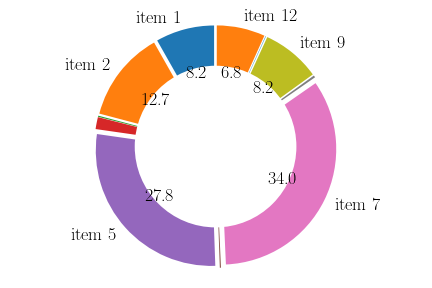
\includegraphics[scale=0.5]{../output/fig/fig2_8-K_before.png}
%		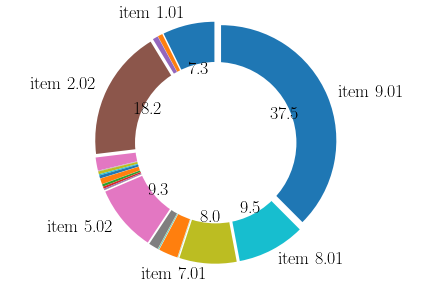
\includegraphics[scale=0.5]{../output/fig/fig2_8-K_after.png}
%	\end{center}
%\end{figure}
%
%Figure 2 illustrates the 8-K item distribution before (left) and after (right) August 23 of 2004. Each share of pie chart shows the percentage of corporate events reported under each 8-K items. See 8-K item list in \hyperref[appa]{Appendix A}.

\newpage
%%%%%%%%%%%%%% Table 1: Sample Selection Process
\begin{landscape}
\begin{table}[htbp] \label{T1}
  \centering
    \begin{tabular}{lcc}
    \multicolumn{3}{c}{\textbf{Table 1. Sample Selection Process}} \\ 
      & &  \\
    \multicolumn{3}{c}{10-Q} \\
     &   \multicolumn{2}{c}{Numer of observations}\\
      & &  \\
    Retrieved from EDGAR & & 575,579 \\
    After merging with COMP and CRSP data & & 303,034 \\
    (-) Number of obs. from utility and financial firms & 82,612 & \\
    (-) Number of firm-quarters with missing values in SIC, SIZE, MTB, LEV, & & \\
    \hspace{5mm}or with non-positive total assets or book value of equity or common shares outstanding, & & \\
    \hspace{5mm}or with common share price less than \$1 & 26,450 & \\
    (-) Number of obs. with total words less than 1\% percentile (1,236 words) & 1,940 & \\
    (-) Number of obs. that contain negative or larger than 99\% TLAG & 1,696 & \\
    \bottomrule
    After dropping obs. with missing values in key variables and screening & & 190,336 \\
    After merging with I\textbackslash{}B\textbackslash{}E\textbackslash{}S and segment data & & 110,062 \\
    (-) Number of obs. that contain missing EARN, STD\_EARN and AF & 18,456 & \\
    \bottomrule
    Full 10-Q sample & & \textbf{91,606} \\
      & &  \\
    \multicolumn{3}{c}{8-K} \\
     &   \multicolumn{2}{c}{Numer of observations}\\
      & &  \\
    Retrieved from EDGAR & & 1,489,626 \\
    After merging and matching with COMP and CRSP data  & & 442,611 \\
    (-) Number of obs. from utility and financial firms & 112,739 & \\
    (-) Number of firm-quarters with missing values in SIC, SIZE, MTB, LEV, & & \\
    \hspace{5mm}or with non-positive total assets or book value of equity or common shares outstanding, & & \\
    \hspace{5mm}or with common share price less than \$1 & 48,230 & \\
    (-) Number of obs. with total words less than 1\% percentile (133 words) & 2,776 & \\
    (-) Number of obs. that are reversals of previous news day & 5,132 & \\
    \bottomrule
    After dropping obs. with missing values in key variables and screening  & & 273,734 \\
    After dropping obs. with negative or larger than 99\% percentile TLAG &  &  \\
    (Full 8-K sample)& & \textbf{119,615} \\
    After dropping obs. with TLAG larger than four (five) days after (before) the 8-K reform &  & \\
    (Restricted 8-K sample) &  & \textbf{40,700} 
    \end{tabular}%
\end{table}%

\end{landscape}

\newpage
%%%%%%%%%%%%%%%%%%%%%%%%% TABLE 2 Panel A + TABLE 2 Panel B
%\begin{landscape}
% Table generated by Excel2LaTeX from sheet 'T2PA '
\begin{table}[htbp] \label{T2PA}
  \centering
    \begin{tabular}{lcccccccc}
    \multicolumn{9}{c}{\textbf{Table 2. Panel A: Summary Statistics 10-Q}} \\
    \midrule
    \midrule
      & count & mean & std & min & 25\% & 50\% & 75\% & max \\
    \midrule
    \textbf{Textual Variables} &   &   &   &   &   &   &   &  \\
    NW & 115980 & 9.165 & 0.745 & 7.121 & 8.713 & 9.246 & 9.665 & 12.865 \\
    nw & 115980 & 12399 & 10137 & 1237 & 6081 & 10362 & 15752 & 386416 \\
    TONE & 115980 & -9.008 & 7.196 & -63.579 & -13.180 & -7.820 & -3.946 & 24.215 \\
    TLAG & 115980 & 38 & 6 & 0 & 35 & 39 & 43 & 51 \\
    READ & 115980 & 36.00 & 40.00 & 14.60 & 17.85 & 19.98 & 33.31 & 253.55 \\
    \textbf{Financial Variables} &   &   &   &   &   &   &   &  \\
    QRET & 115980 & 0.011 & 0.246 & -1.678 & -0.114 & 0.004 & 0.122 & 4.158 \\
    NEG & 115980 & 0.491 & 0.500 & 0 & 0 & 0 & 1 & 1 \\
    SIZE & 115980 & 6.676 & 1.792 & 3.073 & 5.387 & 6.546 & 7.816 & 11.516 \\
    MTB & 115980 & 3.749 & 4.328 & 0.397 & 1.524 & 2.443 & 4.140 & 30.010 \\
    LEV & 115980 & 0.205 & 0.187 & 0.000 & 0.016 & 0.179 & 0.332 & 0.722 \\
    AF & 115980 & 0.044 & 0.090 & -0.410 & 0.022 & 0.049 & 0.077 & 0.327 \\
    AFE & 115980 & -0.009 & 0.044 & -0.301 & -0.007 & 0.000 & 0.003 & 0.081 \\
    BUSSEG & 115980 & 0.982 & 0.553 & 0.693 & 0.693 & 0.693 & 1.099 & 2.773 \\
    GEOSEG & 115980 & 1.049 & 0.662 & 0.693 & 0.693 & 0.693 & 1.099 & 3.219 \\
    AGE & 115980 & 8.303 & 1.081 & 5.620 & 7.574 & 8.446 & 9.106 & 10.317 \\
    EARN & 115980 & 0.001 & 0.047 & -0.224 & -0.002 & 0.011 & 0.022 & 0.084 \\
%    $\Delta$EARN & 115980 & 0.002 & 0.031 & -0.126 & -0.006 & 0.001 & 0.008 & 0.150 \\
    STD\_EARN & 115980 & 0.020 & 0.030 & 0.001 & 0.005 & 0.009 & 0.022 & 0.190 \\
    STD\_QRET & 115980 & 0.086 & 0.068 & 0.007 & 0.039 & 0.068 & 0.112 & 0.367 \\
%    LOSS & 115980 & 0.242 & 0.429 & 0 & 0 & 0 & 0 & 1 \\
    \bottomrule
    \bottomrule
    \end{tabular}%
\end{table}%

% Table generated by Excel2LaTeX from sheet 'T2PC'
\begin{table}[H]   \label{T2PB}%
  \begin{center}
  	\begin{tabular}{lccccccccc}
  		\multicolumn{10}{c}{\textbf{Table 2. Panel B: Summary Statistics by 8-K Item}} \\
  		\midrule
  		\midrule
  		Item & \multicolumn{1}{c}{count} & \multicolumn{1}{c}{percent} & \multicolumn{1}{c}{tlag} & \multicolumn{1}{c}{TONE} & \multicolumn{1}{c}{nw} & \multicolumn{1}{c}{n8k} & \multicolumn{1}{c}{nitem} & \multicolumn{1}{c}{nexhibit} & \multicolumn{1}{c}{ngraph}\\
  		\midrule
  		\multicolumn{10}{c}{Before August 23, 2004} \\
  		\midrule
  		1: Changes in Control & 2712 & 8.35\% & 17 & -1.01 & 1076 & 1.04 & 3.48 & 1.05 & 0.47 \\
  		\: \,\, of Registrant & &  &  &  & & & & & \\
  		2: Acquisition or & 4074 & 12.55\% & 22 & -4.35 & 7146 & 1.04 & 3.05 & 1.59 & 0.31 \\
  		\: \,\, Disposition of Assets & &  &  &  & & & & & \\
  		3: Bankruptcy or & 54 & 0.17\% & 28 & -3.84 & 12217 & 1.11 & 1.56 & 1.74 & 0.00 \\
  		\: \,\, Receivership & &  &  &  & & & & & \\
  		4: Changes in Registrant's & 383 & 1.18\% & 24 & -9.64 & 1217 & 1.03 & 1.82 & 0.95 & 0.02 \\
  		\: \,\, Certifying Accountant & &  &  &  & & & & & \\
  		\textbf{5: Other Events} & \textbf{8909} & \textbf{27.44\%} & \textbf{20} & \textbf{-2.94} & \textbf{4272} & \textbf{1.02} & \textbf{1.81} & \textbf{1.34} & \textbf{0.10} \\
  		6: Resignation of & 34 & 0.10\% & 23 & -9.34 & 9247 & 1.03 & 2.21 & 2.03 & 0.06 \\
  		\: \,\, Registrant's Directors & &  &  &  & & & & & \\
  		7: Financial Statements & 10942 & 33.70\% & 20 & -3.18 & 5169 & 1.02 & 2.33 & 1.58 & 0.38 \\
  		\: \,\, and Exhibits & &  &  &  & & & & & \\
  		8: Change in Fiscal Year & 71 & 0.22\% & 29 & -2.15 & 6068 & 1.01 & 1.66 & 1.63 & 0.03 \\
  		\textbf{9: Reg FD} & \textbf{2966} & \textbf{9.13\%} & \textbf{16} & \textbf{-1.28} & \textbf{549} & \textbf{1.04} & \textbf{1.94} & \textbf{1.10} & \textbf{1.35} \\
  		10: Amendments to the & 6 & 0.02\% & 27 & 0.09 & 289 & 1.17 & 3.50 & 1.00 & 7.17 \\
  		\quad\:\, Registrant's & &  &  &  & & & & & \\
  		\quad\:\, Code of Ethics & &  &  &  & & & & & \\
  		11: Temporary Suspension & 18 & 0.06\% & 20 & -3.40 & 310 & 1.06 & 2.83 & 0.89 & 0.00 \\
  		\quad\:\, of Trading & &  &  &  & & & & & \\
  		\textbf{12: Results of Operation} & \textbf{2303} & \textbf{7.09\%} & \textbf{16} & \textbf{-0.62} & \textbf{329} & \textbf{1.04} & \textbf{3.86} & \textbf{1.12} & \textbf{0.54} \\
  		\midrule
  		\multicolumn{10}{c}{After August 23, 2004 (included)} \\
  		\midrule
  		1: Registrant's Business & 10825 & 7.58\% & 15 & -3.44 & 839 & 1.08 & 2.85 & 1.84 & 1.48 \\
  		\: \,\, and Operations & &  &  &  & & & & & \\
  		2: Financial Information & 31595 & 22.11\% & 13 & 1.02 & 463 & 1.05 & 2.41 & 1.30 & 2.19 \\
  		\textbf{2.02: Results of} & \textbf{27022} & \textbf{18.91\%} & \textbf{12} & \textbf{1.95} & \textbf{404} & \textbf{1.05} & \textbf{2.29} & \textbf{1.22} & \textbf{2.28} \\
  		\: \,\, Operation & &  &  &  & & & & & \\
  		3: Securities and & 1728 & 1.21\% & 13 & -4.26 & 1129 & 1.12 & 3.69 & 2.41 & 1.92 \\
  		\: \,\, Trading Markets & &  &  &  & & & & & \\
  		4: Matters Related & 478 & 0.33\% & 16 & -10.32 & 770 & 1.09 & 2.32 & 1.19 & 0.57 \\
  		\: \,\, to Accountants & &  &  &  & & & & & \\
  		\: \,\, and Financial & &  &  &  & & & & & \\
  		\: \,\, Statements & &  &  &  & & & & & \\
  		5: Corporate Governance & 19494 & 13.64\% & 16 & 0.09 & 587 & 1.06 & 2.06 & 0.96 & 0.65 \\
  		\: \,\, and Management & &  &  &  & & & & &  \\
  		6: Asset-Backed Securities & 2 & 0.00\% & 7 & 2.20 & 200 & 1.00 & 2.00 & 1.00 & 0.00 \\
  		\textbf{7: Reg FD} & \textbf{11844} & \textbf{8.29\%} & \textbf{11} & \textbf{0.33} & \textbf{562} & \textbf{1.09} & \textbf{2.65} & \textbf{1.36} & \textbf{8.97} \\
  		\textbf{8: Other Events} & \textbf{13009} & \textbf{9.11\%} & \textbf{12} & \textbf{-0.85} & \textbf{569} & \textbf{1.09} & \textbf{2.46} & \textbf{1.38} & \textbf{1.98} \\
  		9: Financial Statements & 53896 & 37.72\% & 13 & 0.49 & 500 & 1.05 & 2.41 & 1.39 & 3.00 \\
  		\: \,\, and Exhibits & &  &  &  & & & & & \\
  		\bottomrule
  		\bottomrule
  	\end{tabular}%
  \end{center}
	\begin{footnotesize}
		\noindent Table 2 Panel B presents the descriptive statistics of key textual variables by 8-K items. Count represents the total number of times that each 8-K item is reported. Percent represents the percentage of each 8-K item calculated based on their number of appearances. See \hyperref[appc]{Appendix C} for other variable definitions. Column tlag, TONE, nw, n8k, nitem, nexhibit and ngraph report the mean value of the corresponding variable in each 8-K item group. See \hyperref[appa]{Appendix A} for 8-K item descriptions. Voluntary 8-K items are in bold.
	\end{footnotesize}
\end{table}%

%\end{landscape}

\newpage
%%%%%%%%%%%%%%%%%%%%%%%%% TABLE C
%\begin{landscape}
% Table generated by Excel2LaTeX from sheet 'T2PC'
\begin{table}[H]   \label{T2PC}%
  \begin{center}
  	\begin{tabular}{lccccc}
  		\multicolumn{6}{c}{\textbf{Table 2. Panel C: Summary Statistics by 8-K Item}} \\
  		\midrule
  		\midrule
  		Item & \multicolumn{1}{c}{\# of appearance} & \multicolumn{1}{c}{\% of appearance} & \multicolumn{1}{c}{nw} & \multicolumn{1}{c}{TONE} & \multicolumn{1}{c}{TLAG} \\
  		\midrule
  		\multicolumn{6}{l}{Before August 23, 2004} \\
  		\midrule
  		1: Changes in Control & 4377 & 8.21\% & 1195 & -1.22 & 17.29 \\
  		\: \,\, of Registrant & &  &  &  & \\
  		2: Acquisition or Disposition & 6773 & 12.70\% & 7183 & -4.65 & 22.34 \\
  		\: \,\, of Assets & &  &  &  & \\
  		3: Bankruptcy or Receivership & 85 & 0.16\% & 9920 & -4.05 & 27.89 \\
  		4: Changes in Registrant's & 895 & 1.68\% & 1128 & -9.50 & 24.71 \\
  		\: \,\, Certifying Accountant & &  &  &  & \\
  		\textbf{5: Other Events} & \textbf{14836} & \textbf{27.82\%} & \textbf{4431} & \textbf{-3.14} & \textbf{20.49} \\
  		6: Resignation of Registrant's & 84 & 0.16\% & 8052 & -11.32 & 27.98 \\
  		\: \,\, Directors & &  &  &  & \\
  		7: Financial Statements & 18111 & 33.96\% & 5239 & -3.48 & 20.70 \\
  		\: \,\, and Exhibits & &  &  &  & \\
  		8: Change in Fiscal Year & 153 & 0.29\% & 3322 & -0.95 & 27.59 \\
  		\textbf{9: Reg FD} & \textbf{4379} & \textbf{8.21\%} & \textbf{571} & \textbf{-1.25} & \textbf{15.56} \\
  		10: Amendments to the & 11 & 0.02\% & 353 & -2.93 & 19.64 \\
  		\quad\:\, Registrant's Code of Ethics & &  &  &  & \\
  		11: Temporary Suspension & 26 & 0.05\% & 309 & -3.43 & 19.31 \\
  		\: \,\, of Trading & &  &  &  & \\
  		\textbf{12: Results of Operation} & \textbf{3608} & \textbf{6.76\%} & \textbf{316} & \textbf{-0.61} & \textbf{15.98} \\
  		\midrule
  		\multicolumn{6}{l}{After August 23, 2004 (included)} \\
  		\midrule
  		1: Registrant's Business & 15672 & 7.95\% & 797 & -3.43 & 14.96 \\
  		\: \,\, and Operations & &  &  &  & \\
  		2: Financial Information & 42226 & 21.42\% & 449 & 1.03 & 12.76 \\
  		\textbf{2.02: Results of Operation} & \textbf{35910} & \textbf{18.22\%} & \textbf{395} & \textbf{1.97} & \textbf{12.43} \\
  		3: Securities and Trading Markets & 3063 & 1.55\% & 1081 & -4.10 & 13.03 \\
  		4: Matters Related to Accountants & 888 & 0.45\% & 779 & -10.14 & 16.54 \\
  		\: \,\, and Financial Statements & &  &  &  & \\
  		5: Corporate Governance & 26776 & 13.58\% & 539 & -0.06 & 15.76 \\
  		\: \,\, and Management & &  &  &  & \\
  		6: Asset-Backed Securities & 3 & 0.00\% & 211 & 2.91 & 14.33 \\
  		\textbf{7: Reg FD} & \textbf{15795} & \textbf{8.01\%} & \textbf{555} & \textbf{0.29} & \textbf{11.04} \\
  		\textbf{8: Other Events} & \textbf{18734} & \textbf{9.50\%} & \textbf{567} & \textbf{-0.86} & \textbf{11.66} \\
  		9: Financial Statements & 73982 & 37.53\% & 488 & 0.40 & 12.82 \\
  		\: \,\, and Exhibits & &  &  &  & \\
  		\bottomrule
  		\bottomrule
  	\end{tabular}%
  \end{center}
	\begin{footnotesize}
		\noindent Table 2 Panel C presents the descriptive statistics of key textual variables by 8-K items. Number of appearance represents the total number of times that each 8-K item is reported. Percentage of appearance represents the percentage of each 8-K item calculated based on the number of appearance. See \hyperref[appb]{Appendix B} for other variable definitions. Column nw, TONE and TLAG report the mean value of the corresponding variable in each 8-K item group. See \hyperref[appa]{Appendix A} for 8-K item descriptions. Voluntary 8-K items are in bold.
	\end{footnotesize}
\end{table}%

%\end{landscape}

%%%%%%%%%%%%%%%%%%%%%%%%% TABLE 2 Panel D 
\newpage
%\begin{landscape}
% Table generated by Excel2LaTeX from sheet 'T2PD'
\begin{table}[H] \label{T2PD}
	\centering
	\begin{tabular}{lrrrrrrrrr}
		\multicolumn{9}{c}{\textbf{Table 2. Panel D: Correlation Matrix 10-Q}} \\
		\midrule
		\midrule
		& \multicolumn{1}{c}{(1)} & \multicolumn{1}{c}{(2)} & \multicolumn{1}{c}{(3)} & \multicolumn{1}{c}{(4)} & \multicolumn{1}{c}{(5)} & \multicolumn{1}{c}{(6)} & \multicolumn{1}{c}{(7)} & \multicolumn{1}{c}{(8)} \\
		\midrule
		(1) NW &  & -0.456 & -0.192 & -0.083 & -0.007 & 0.002 & 0.255 & 0.058 & \\
		(2) TONE & -0.482 &  & 0.016 & 0.086 & 0.020 & -0.021 & -0.062 & -0.013 &  \\
		(3) TLAG & -0.263 & 0.021 &  & 0.048 & -0.022 & 0.034 & -0.331 & -0.023 & \\
		(4) READ & -0.252 & 0.169 & 0.125 &  & -0.016 & 0.016 & -0.014 & -0.037 & \\
		(5) QRET & -0.007 & 0.028 & -0.032 & -0.029 &  & -0.684 & -0.064 & -0.029 & \\
		(6) NEG & 0.003 & -0.024 & 0.033 & 0.028 & -0.866 &  & 0.000 & 0.014 &  \\
		(7) SIZE & 0.264 & -0.047 & -0.333 & -0.078 & -0.024 & -0.001 &  & 0.247 & \\
		(8) MTB & 0.046 & 0.040 & -0.042 & -0.026 & -0.055 & 0.033 & 0.382 &  &  \\
		(9) LEV & 0.014 & 0.076 & 0.000 & 0.075 & 0.003 & -0.004 & 0.143 & -0.111 &  \\
		(10) AF & -0.018 & 0.062 & -0.125 & 0.035 & -0.087 & 0.072 & 0.026 & -0.299 &  \\
		(11) AFE & 0.040 & 0.099 & -0.149 & -0.023 & 0.181 & -0.157 & 0.232 & 0.226 &  \\
		(12) AGE & -0.035 & 0.063 & -0.232 & 0.071 & 0.011 & -0.015 & 0.336 & -0.081 &  \\
		(13) EARN & -0.139 & 0.223 & -0.146 & 0.065 & 0.114 & -0.098 & 0.299 & 0.282 &  \\
		%    (14) $\Delta$EARN & 0.005 & 0.011 & -0.014 & -0.006 & 0.059 & -0.041 & -0.013 & 0.019 & 0.024 & 0.016 & 0.091 & 0.003 & 0.299 &  & 0.055 & 0.015 \\
		(14) STD\_EARN & 0.092 & -0.194 & 0.153 & -0.052 & -0.024 & 0.028 & -0.281 & 0.093 &  \\
		(15) STD\_QRET & -0.047 & -0.083 & 0.214 & -0.023 & 0.128 & -0.088 & -0.325 & -0.041 & \\
		%    (17) ABTONE & -0.404 & 0.944 & 0.020 & 0.139 & 0.000 & -0.001 & 0.017 & 0.063 & 0.076 & -0.004 & 0.025 & 0.004 & 0.063 & -0.009 & -0.066 & -0.010 &  \\
		\bottomrule
		\bottomrule
	\end{tabular}%
\end{table}%
% Table generated by Excel2LaTeX from sheet 'T2PD'
\begin{table}[H]
  \begin{center}
  	\begin{tabular}{lrrrrrrr}
  		\multicolumn{8}{c}{\textbf{Table 2. Panel D: Correlation Matrix 10-Q (Continued) }} \\
  		\midrule
  		\midrule
  		& \multicolumn{1}{c}{(9)} & \multicolumn{1}{c}{(10)} & \multicolumn{1}{c}{(11)} & \multicolumn{1}{c}{(12)} & \multicolumn{1}{c}{(13)} & \multicolumn{1}{c}{(14)} & \multicolumn{1}{c}{(15)} \\
  		\midrule
  		(1) NW & 0.036 & -0.068 & 0.011 & -0.040 & -0.116 & 0.091 & -0.030 \\
  		(2) TONE & 0.072 & 0.072 & 0.102 & 0.059 & 0.157 & -0.148 & -0.089 \\
  		(3) TLAG & 0.009 & -0.092 & -0.127 & -0.228 & -0.137 & 0.121 & 0.189 \\
  		(4) READ & 0.063 & 0.045 & 0.002 & 0.088 & 0.059 & -0.047 & -0.051 \\
  		(5) QRET & 0.002 & -0.018 & 0.155 & 0.002 & 0.063 & 0.011 & 0.266 \\
  		(6) NEG & -0.002 & 0.015 & -0.124 & -0.018 & -0.071 & 0.016 & -0.118 \\
  		(7) SIZE & 0.101 & 0.079 & 0.267 & 0.345 & 0.259 & -0.198 & -0.310 \\
  		(8) MTB & 0.033 & -0.167 & 0.128 & -0.094 & -0.040 & 0.163 & 0.037 \\
  		(9) LEV &  & 0.168 & -0.068 & 0.102 & 0.040 & -0.125 & -0.072 \\
  		(10) AF & 0.251 &  & 0.057 & 0.202 & 0.472 & -0.256 & -0.145 \\
  		(11) AFE & -0.052 & 0.060 &  & 0.072 & 0.241 & -0.143 & -0.159 \\
  		(12) AGE & 0.146 & 0.211 & 0.060 &  & 0.211 & -0.223 & -0.262 \\
  		(13) EARN & -0.073 & 0.247 & 0.357 & 0.172 &  & -0.412 & -0.229 \\
  		%    (14) $\Delta$EARN & 0.005 & 0.011 & -0.014 & -0.006 & 0.059 & -0.041 & -0.013 & 0.019 & 0.024 & 0.016 & 0.091 & 0.003 & 0.299 &  & 0.055 & 0.015 \\
  		(14) STD\_EARN & -0.201 & -0.205 & -0.152 & -0.250 & 0.036 &  & 0.241 \\
  		(15) STD\_QRET & -0.102 & -0.131 & -0.110 & -0.275 & 0.004 & 0.277 & \\
  		%    (17) ABTONE & -0.404 & 0.944 & 0.020 & 0.139 & 0.000 & -0.001 & 0.017 & 0.063 & 0.076 & -0.004 & 0.025 & 0.004 & 0.063 & -0.009 & -0.066 & -0.010 &  \\
  		\bottomrule
  		\bottomrule
  	\end{tabular}%
  \end{center}
	\begin{footnotesize}
		\noindent Table 2 Panel D presents the correlation matrix of key variables in 10-Q sample. Pearson (Spearman) correlations are exhibited above (below) the diagonal. See \hyperref[appb]{Appendix B} for variable definitions. READ and all financial variables except returns are winsorized at 1\% and 99\% level. 
	\end{footnotesize}
\end{table}%
%\end{landscape}

%%%%%%%%%%%%%%%%%%%%%%%%% TABLE 2 Panel E
\newpage
\begin{landscape}
% Table generated by Excel2LaTeX from sheet 'T2PE'
\begin{table}[H] \label{T2PE}
  \begin{center}
  	\begin{tabular}{lrrrrrrrrrrr}
  		\multicolumn{12}{c}{\textbf{Table 2. Panel E: Correlation Matrix 8-K}} \\
  		\midrule
  		\midrule
  		& \multicolumn{1}{c}{(1)} & \multicolumn{1}{c}{(2)} & \multicolumn{1}{c}{(3)} & \multicolumn{1}{c}{(4)} & \multicolumn{1}{c}{(5)} & \multicolumn{1}{c}{(6)} & \multicolumn{1}{c}{(7)} & \multicolumn{1}{c}{(8)} & \multicolumn{1}{c}{(9)} & \multicolumn{1}{c}{(10)} & \multicolumn{1}{c}{(11)} \\
  		\midrule
  		(1) NW & & -0.425 & 0.133 & 0.154 & 0.164 & 0.021 & -0.015 & 0.011 & -0.024 & 0.042 & 0.075 \\
  		(2) TONE & -0.414 & & -0.079 & -0.024 & -0.081 & 0.003 & 0.015 & -0.011 & 0.069 & 0.004 & -0.035 \\
  		(3) TLAG & 0.119 & -0.110 & & -0.041 & -0.056 & -0.016 & -0.037 & 0.038 & -0.093 & -0.006 & -0.035 \\
  		(4) N8K & 0.206 & -0.043 & -0.059 & & 0.432 & 0.017 & 0.011 & -0.006 & 0.032 & 0.000 & 0.022 \\
  		(5) NITEM & 0.184 & -0.104 & -0.093 & 0.296 & & 0.009 & 0.006 & -0.004 & 0.014 & -0.005 & 0.026 \\
  		(6) DRET & -0.001 & 0.009 & -0.019 & 0.006 & 0.003 & & 0.709 & -0.572 & -0.028 & 0.004 & 0.004 \\
  		(7) $\Delta$DRET & -0.016 & 0.019 & -0.049 & -0.005 & -0.005 & -0.780 & & -0.863 & 0.069 & -0.006 & 0.013 \\
  		(8) BN & 0.012 & -0.012 & 0.049 & -0.005 & -0.005 & -0.780 & -0.863 & & -0.032 & 0.002 & -0.009 \\
  		(9) SIZE & 0.029 & 0.075 & -0.113 & 0.032 & 0.024 & 0.025 & 0.080 & -0.032 & & 0.192 & 0.167 \\
  		(10) MTB & 0.047 & 0.026 & -0.016 & 0.003 & -0.007 & 0.005 & 0.009 & -0.003 & 0.350 & & 0.086 \\
  		(11) LEV & 0.081 & -0.043 & -0.041 & 0.022 & 0.025 & 0.014 & 0.022 & -0.011 & 0.213 & -0.039 & \\
  		\bottomrule
  		\bottomrule
  	\end{tabular}%
  \end{center}
	\begin{footnotesize}
		\noindent Table 2 Panel E present the correlation matrix of key variables in 8-K sample. Pearson (Spearman) correlations are exhibited above (below) the diagonal. See \hyperref[appb]{Appendix B} for variable definitions. All financial variables except returns are winsorized at 1\% and 99\% level. 
	\end{footnotesize}
\end{table}%

\end{landscape}

%%%%%%%%%%%%%%%%%%%%%%%%% TABLE 3 Panel A
\newpage
%\begin{landscape}
% Table generated by Excel2LaTeX from sheet 'T3PA'
\begin{table}[H] \label{T3PA}
	\begin{center}
		\begin{tabular}{lcccccc}
			\multicolumn{7}{c}{\textbf{Table 3. Panel A: Is 10-Q Narrative Disclosure Conservative?}} \\
			\toprule
			\toprule
			& (1) & (2) & (3) & (4) & (5) & (6) \\
			Dep. Variables & NW & NW & TONE & TONE & TLAG & TLAG \\
			\midrule
			&   &   &   &   &   &  \\
			QRET & 0.039*** & 0.029** & -0.279** & 0.335** & -0.081 & -0.318*** \\
			& (3.23) & (2.21) & (-2.04) & (2.58) & (-0.78) & (-2.72) \\
			NEG & 0.006 & 0.007 & -0.113** & -0.116** & 0.027 & 0.039 \\
			& (1.29) & (1.45) & (-2.20) & (-2.31) & (0.73) & (1.03) \\
			\rowcolor[rgb]{ .933,  .925,  .882} \textit{(Pred. Sign)} & (-) & (-) & (+) & (+) & (+) & (+) \\
			\rowcolor[rgb]{ .933,  .925,  .882} QRET$\times$NEG & -0.145*** & -0.075*** & 2.103*** & 0.760*** & -0.771*** & -0.189 \\
			\rowcolor[rgb]{ .933,  .925,  .882}   & (-6.05) & (-3.36) & (6.67) & (2.82) & (-4.07) & (-1.04) \\
			SIZE &   & 0.035*** &   & 0.469*** &   & -0.135** \\
			&   & (3.79) &   & (5.57) &   & (-2.06) \\
			MTB &   & -0.007*** &   & 0.077*** &   & -0.023** \\
			&   & (-5.53) &   & (4.34) &   & (-1.98) \\
			LEV &   & 0.332*** &   & -1.260*** &   & 0.748** \\
			&   & (9.76) &   & (-2.77) &   & (2.16) \\
			EARN &   & -0.653*** &   & 15.058*** &   & -5.455*** \\
			&   & (-4.27) &   & (5.93) &   & (-6.21) \\
			STD\_RET &   & 0.110*** &   & -1.921*** &   & 0.844*** \\
			&   & (3.54) &   & (-5.72) &   & (3.38) \\
			STD\_EARN &   & 0.672*** &   & -7.792*** &   & 5.217*** \\
			&   & (7.42) &   & (-5.42) &   & (6.20) \\
			AGE &   & -0.065*** &   & -0.046 &   & 0.199 \\
			&   & (-4.23) &   & (-0.20) &   & (1.32) \\
			BUSSEG &   & 0.015 &   & 0.460** &   & 0.094 \\
			&   & (1.02) &   & (2.10) &   & (0.52) \\
			GEOSEG &   & -0.039*** &   & 0.266 &   & -0.361** \\
			&   & (-3.24) &   & (1.26) &   & (-1.97) \\
			AF &   & -0.060 &   & -1.866* &   & -1.021* \\
			&   & (-0.65) &   & (-1.86) &   & (-1.73) \\
			AFE &   & -0.192*** &   & 5.624*** &   & -2.397*** \\
			&   & (-3.60) &   & (9.06) &   & (-6.15) \\
			Constant & 8.139*** & 8.468*** & -16.652*** & -19.772*** & 44.074*** & 43.617*** \\
			& (233.65) & (65.88) & (-35.13) & (-11.06) & (113.45) & (36.70) \\
			&   &   &   &   &   &  \\
			Observations & 91,606 & 91,606 & 91,606 & 91,606 & 91,606 & 91,606 \\
			Adjusted R-squared & 0.649 & 0.653 & 0.557 & 0.570 & 0.613 & 0.616 \\
			\bottomrule
			\bottomrule
		\end{tabular}%
	\end{center}
		\begin{footnotesize}
			\setcounter{equation}{0}
			\begin{equation}
				TEX_{i,t}=\beta_0+\beta_1QRET_{i,t}+\beta_2NEG_{i,t}+\beta_3QRET_{i,t}\times NEG_{i,t}+\sum\beta_nCONTROLS_{i,t}+\epsilon_{i,t}
			\end{equation}
			
			\noindent Table 3 Panel A presents the regression results of Equation (1). TEX represents a vector of textual properties that consists of number of words (NW), tone (TONE) and reporting time lag (TLAG). CONTROLS denotes a vector of control variables. See \hyperref[appb]{Appendix B} for variable definitions. All financial variables except returns are winsorized at 1\% and 99\% level. All regressions include firm and time fixed effects and standard errors are clustered at industry level identified by 4-digit SIC codes. ***, ** and * indicate significance at the 1\%, 5\% and 10\% levels in a two-tailed test.
		\end{footnotesize}
\end{table}%
%\end{landscape}

%%%%%%%%%%%%%%%%%%%%%%%%% TABLE 3 Panel B
\newpage
% Table generated by Excel2LaTeX from sheet 'T3PB'
\begin{table}[H] \label{T3PB}
	\begin{center}
		\begin{tabular}{lcccc}
			\multicolumn{5}{c}{\textbf{Table 3. Panel B: Are Lengthier 10-Qs Less Readable?}} \\
			\midrule
			\midrule
			& (1) & (2) & (3) & (4) \\
			Dep. Variables & READ & READ & READ & READ \\
			\midrule
			&   &   &   &  \\
			NW & 13.048*** & 13.298*** & 13.407*** & 13.697*** \\
			& (21.59) & (21.73) & (18.50) & (18.74) \\
			QRET & -1.001 & -0.471 & 8.889 & 11.146 \\
			& (-1.49) & (-0.74) & (0.82) & (1.03) \\
			NEG & 0.012 & 0.028 & -0.597 & -0.597 \\
			& (0.05) & (0.11) & (-0.14) & (-0.14) \\
			\rowcolor[rgb]{ .933,  .925,  .882}\textit{(Pred. Sign)} & (-) & (-) & (?) & (?) \\
			\rowcolor[rgb]{ .933,  .925,  .882} QRET$\times$NEG & 3.686** & 2.341* & -37.674* & -43.311* \\
			\rowcolor[rgb]{ .933,  .925,  .882} & (2.52) & (1.66) & (-1.66) & (-1.92) \\
			NW$\times$NEG &   &   & 0.067 & 0.068 \\
			&   &   & (0.14) & (0.14) \\
			QRET$\times$NW &   &   & -1.093 & -1.285 \\
			&   &   & (-0.91) & (-1.07) \\
			\rowcolor[rgb]{ .933,  .925,  .882} \textit{(Pred. Sign)} & & &  (-) &  (-)\\
			\rowcolor[rgb]{ .933,  .925,  .882} QRET$\times$NEG$\times$NW &   &   &  4.568* &  5.045** \\
			\rowcolor[rgb]{ .933,  .925,  .882} &   &   & (1.81) & (2.02) \\
			&   &   &   &  \\
			Observations & 91,606 & 91,606 & 91,606 & 91,606 \\
			Adjusted R-squared & 0.461 & 0.462 & 0.461 & 0.462 \\
			Controls & NO & YES & NO & YES \\
			\bottomrule
			\bottomrule
		\end{tabular}%
	\end{center}
		\begin{footnotesize}
			\setcounter{equation}{0}
			\begin{equation*}
				READ_{i,t}=\beta_0+\beta_1NW_{i,t}+\beta_2QRET_{i,t}+\beta_3NEG_{i,t}+\beta_4QRET_{i,t}\times NEG_{i,t}+\sum\beta_nCONTROLS_{i,t}+\epsilon_{i,t}
			\end{equation*}
			
			\begin{equation*}
				\begin{split}
					READ_{i,t}=\beta_0&+\beta_1NW_{i,t}+\beta_2QRET_{i,t}+\beta_3NEG_{i,t}\\
					&+\beta_4QRET_{i,t}\times NEG_{i,t}+\beta_5NW_{i,t}\times NEG_{i,t}+\beta_6QRET_{i,t}\times NW_{i,t}\\
					&+\beta_7QRET_{i,t}\times NEG_{i,t}\times NW_{i,t}+\sum\beta_nCONTROLS_{i,t}+\epsilon_{i,t}
				\end{split}
			\end{equation*}
			
			\noindent Table 3 Panel B presents the regression results of the above models. CONTROLS denotes a vector of control variables, including SIZE, MTB, LEV, EARN, STD\_RET, STD\_EARN, AGE, BUGSSEG, GEOSSEG, AF, AFE. See \hyperref[appb]{Appendix B} for variable definitions. READ and all financial variables except returns are winsorized at 1\% and 99\% level. All regressions include firm and time fixed effects and standard errors are clustered at industry level identified by 4-digit SIC codes. ***, ** and * indicate significance at the 1\%, 5\% and 10\% levels in a two-tailed test.
		\end{footnotesize}
\end{table}%


%%%%%%%%%%%%%%%%%%%%%%%%% TABLE 4 Panel A
\newpage
%\begin{landscape}
% Table generated by Excel2LaTeX from sheet 'T4PA'
\begin{table}[H] \label{T4PA}%
	\begin{center}
		\begin{tabular}{lcccccc}
			\multicolumn{7}{c}{\textbf{Table 4. Panel A: Is 8-K Narrative Disclosure Conservative?}} \\
			\midrule
			\midrule
			& (1) & (2) & (3) & (4) & (5) & (6) \\
			Dep. Variables & NW & NW & TONE & TONE & TLAG & TLAG \\
			\midrule
			&   &   &   &   &   &  \\
			$\Delta$DRET & 0.062* & 0.050 & -1.066*** & -0.878** & -13.541*** & -13.924*** \\
			& (1.78) & (1.43) & (-2.87) & (-2.48) & (-10.81) & (-10.65) \\
			BN & 0.007 & 0.007 & -0.091 & -0.082 & 0.206 & 0.190 \\
			& (1.24) & (1.15) & (-1.42) & (-1.30) & (1.13) & (1.02) \\
			\rowcolor[rgb]{ .933,  .925,  .882} \textit{(Pred. Sign)} & (-) & (-) & (+) & (+) & (+) & (+) \\
			\rowcolor[rgb]{ .933,  .925,  .882} $\Delta$DRET$\times$BN & -0.129** & -0.108** & 2.178*** & 1.843*** & 20.163*** & 20.861*** \\
			\rowcolor[rgb]{ .933,  .925,  .882}   & (-2.58) & (-2.15) & (3.14) & (2.90) & (11.85) & (11.64) \\
			SIZE &   & -0.010 &   & 0.140*** &   & -0.493*** \\
			&   & (-1.47) &   & (2.66) &   & (-5.22) \\
			MTB &   & 0.003*** &   & -0.009 &   & 0.016 \\
			&   & (2.72) &   & (-1.27) &   & (0.78) \\
			LEV &   & 0.039 &   & -0.872*** &   & -1.867*** \\
			&   & (1.19) &   & (-2.94) &   & (-3.70) \\
			Constant & 7.242*** & 7.280*** & -6.358*** & -6.952*** & 30.067*** & 33.040*** \\
			& (33.38) & (33.20) & (-3.81) & (-4.25) & (7.54) & (8.16) \\
			&   &   &   &   &   &  \\
			Observations & 119,616 & 119,616 & 119,616 & 119,616 & 119,616 & 119,616 \\
			Adjusted R-squared & 0.447 & 0.447 & 0.157 & 0.158 & 0.135 & 0.136 \\
			\bottomrule
			\bottomrule
		\end{tabular}%
	\end{center}
		\begin{footnotesize}
			\setcounter{equation}{1}
			\begin{equation}
				TEX_{i,t}=\beta_0+\beta_1\Delta DRET_{i,t-tlag}+\beta_2BN_{i,t-tlag}+\beta_3\Delta DRET_{i,t-tlag}\times 	BN_{i,t-tlag}+\sum\beta_nCONTROLS_{i,t}+\epsilon_{i,t}
			\end{equation}
			
			\noindent Table 4 Panel A presents the regression results of Equation (2). TEX represents a vector of textual properties that consists of number of words (NW), tone (TONE) and reporting time lag (TLAG). CONTROLS denotes a vector of control variables, including SIZE, MTB and LEV. See \hyperref[appb]{Appendix B} for variable definitions. All financial variables except returns are winsorized at 1\% and 99\% level. All regressions include firm and time fixed effects and standard errors are clustered at industry level identified by 4-digit SIC codes. ***, ** and * indicate significance at the 1\%, 5\% and 10\% levels in a two-tailed test.
		\end{footnotesize}
\end{table}%
%\end{landscape}

%%%%%%%%%%%%%%%%%%%%%%%%% TABLE 4 Panel B
\newpage
%\begin{landscape}
% Table generated by Excel2LaTeX from sheet 'T6'
\begin{table}[H] \label{T4PB}%
	\begin{center}
		\begin{tabular}{lcccc}
			\multicolumn{5}{c}{\textbf{Table 4. Panel B. Narrative Conservatism 10-Q Sections}} \\
			\midrule
			\midrule
			Dep. Variables & \multicolumn{2}{c}{TONE} & \multicolumn{2}{c}{NW} \\
			\cmidrule{2-5}
			& (1) & (2) & (3) & (4) \\
			Section & MDA & NFS & MDA & NFS \\
			\midrule
			%&   &   &   &  \\
			QRET & 0.109 & 0.297 & -0.055*** & -0.033* \\
			& (0.64) & (1.15) & (-4.34) & (-1.70) \\
			NEG & -0.123** & 0.014 & -0.012*** & -0.005 \\
			& (-1.98) & (0.17) & (-3.05) & (-1.01) \\
			\rowcolor[rgb]{ .906,  .902,  .902} \textit{(Pred. Sign)} & (+) & (+) & (+) & (+) \\
			\rowcolor[rgb]{ .906,  .902,  .902} QRET$\times$NEG & 1.423*** & 0.882* & 0.102*** & 0.055* \\
			\rowcolor[rgb]{ .906,  .902,  .902} & (4.54) & (1.88) & (4.18) & (1.65) \\
			SIZE & 0.626*** & 0.900*** & -0.030*** & -0.013 \\
			& (4.26) & (5.14) & (-3.36) & (-1.01) \\
			MTB & 0.021 & 0.054** & 0.003** & 0.004*** \\
			& (1.12) & (2.21) & (2.41) & (3.28) \\
			LEV & -0.213 & -0.802 & -0.189*** & -0.362*** \\
			& (-0.33) & (-0.94) & (-5.32) & (-5.88) \\
			EARN & 17.163*** & 12.079*** & 0.470** & 0.693*** \\
			& (5.26) & (5.69) & (2.16) & (3.83) \\
			STD\_EARN & -8.090*** & -6.020** & -0.547*** & -0.816*** \\
			& (-4.64) & (-2.20) & (-3.35) & (-6.19) \\
			BUSSEG & -0.065 & -0.159 & -0.057*** & -0.031 \\
			& (-0.23) & (-0.45) & (-2.93) & (-1.58) \\
			GEOSEG & 0.052 & 0.999*** & 0.063*** & 0.036** \\
			& (0.16) & (2.61) & (3.01) & (1.98) \\
			AF & 1.979* & -0.343 & 0.140 & -0.073 \\
			& (1.86) & (-0.22) & (1.61) & (-0.95) \\
			AFE & 7.938*** & 4.137*** & 0.227*** & 0.243*** \\
			& (7.81) & (3.74) & (3.20) & (3.56) \\
			Constant & -7.264* & -12.393** & -7.167*** & -7.224*** \\
			& (-1.84) & (-2.57) & (-15.46) & (-18.08) \\
			&   &   &   &  \\
			Observations & 48,089 & 48,089 & 48,089 & 48,089 \\
			Adjusted R-squared & 0.559 & 0.579 & 0.734 & 0.816 \\
			\bottomrule
			\bottomrule
		\end{tabular}%
	\end{center}
\begin{footnotesize}
	\setcounter{equation}{1}
	\begin{equation}
		TEX_{i,t}=\beta_0+\beta_1QRET_{i,t}+\beta_2NEG_{i,t}+\beta_3QRET_{i,t}\times NEG_{i,t}+\sum\beta_nCONTROLS_{i,t}+\epsilon_{i,t}
	\end{equation}
	
	\noindent Table 4 Panel B presents the regression results of Equation (2) using subsamples of MD\&A (Column 1 and 3) and NFS (Column 2 and 4) sections. TEX represents a vector of textual properties that consists of NW\_MDA, NW\_NFS, TONE\_MDA and TONE\_NFS. CONTROLS denotes a vector of control variables. See \hyperref[appc]{Appendix C} for variable definitions. All financial variables except returns are winsorized at 1\% and 99\% level. All regressions include firm and year-quarter fixed effects and standard errors are clustered at industry level identified by 4-digit SIC codes. ***, ** and * indicate significance at the 1\%, 5\% and 10\% levels in a two-tailed test.
\end{footnotesize}
\end{table}%
%\end{landscape}

%%%%%%%%%%%%%%%%%%%%%%%%% TABLE 5
\newpage
%\begin{landscape}
% Table generated by Excel2LaTeX from sheet 'T6'
\begin{table}[H]	\label{T5}%
	\begin{center}
		\begin{tabular}{lcccc}
			\multicolumn{5}{c}{\textbf{Table 5. Narrative conservatism in MD\&A and NFS}} \\
			\midrule
			\midrule
			& (1) & (2) & (3) & (4) \\
			Dep. Variables & NW\_MDA & NW\_NFS & TONE\_MDA & TONE\_NFS \\
			\midrule
			&   &   &   &  \\
			QRET & 0.025** & 0.022 & 0.620*** & 0.418 \\
			& (2.14) & (1.12) & (3.87) & (1.52) \\
			NEG & 0.011*** & 0.005 & -0.106* & 0.019 \\
			& (2.80) & (0.95) & (-1.71) & (0.23) \\
			\rowcolor[rgb]{ .933,  .925,  .882} \textit{(Pred. Sign)} & (-) & (-) & (+) & (+) \\
			\rowcolor[rgb]{ .933,  .925,  .882} QRET$\times$NEG & -0.061*** & -0.039 & 0.797** & 0.764 \\
			\rowcolor[rgb]{ .933,  .925,  .882}   & (-2.73) & (-1.19) & (2.54) & (1.63) \\
			SIZE & 0.033*** & 0.014 & 0.596*** & 0.902*** \\
			& (3.66) & (1.10) & (3.97) & (5.10) \\
			MTB & -0.003*** & -0.004*** & 0.026 & 0.053** \\
			& (-2.89) & (-3.42) & (1.45) & (2.18) \\
			LEV & 0.210*** & 0.371*** & -0.369 & -0.730 \\
			& (5.79) & (5.93) & (-0.58) & (-0.86) \\
			EARN & -0.443** & -0.682*** & 16.777*** & 12.026*** \\
			& (-2.09) & (-3.79) & (5.16) & (5.64) \\
			STD\_RET & 0.211*** & 0.078** & -3.703*** & -0.971 \\
			& (4.43) & (1.97) & (-7.39) & (-1.26) \\
			STD\_EARN & 0.450*** & 0.775*** & -7.045*** & -6.091** \\
			& (2.93) & (6.09) & (-4.05) & (-2.25) \\
			AGE & -0.079*** & -0.035* & 0.706*** & -0.176 \\
			& (-3.85) & (-1.66) & (2.93) & (-0.49) \\
			BUSSEG & 0.051*** & 0.029 & -0.008 & -0.172 \\
			& (2.71) & (1.43) & (-0.03) & (-0.49) \\
			GEOSEG & -0.068*** & -0.039** & 0.096 & 0.983** \\
			& (-3.26) & (-2.11) & (0.29) & (2.56) \\
			AF & -0.130 & 0.077 & 1.895* & -0.321 \\
			& (-1.50) & (1.00) & (1.77) & (-0.21) \\
			AFE & -0.235*** & -0.247*** & 7.893*** & 4.031*** \\
			& (-3.31) & (-3.61) & (7.83) & (3.65) \\
			Constant & 7.748*** & 7.483*** & -12.351*** & -11.024** \\
			& (16.47) & (17.89) & (-2.83) & (-2.04) \\
			&   &   &   &  \\
			Observations & 48,089 & 48,089 & 48,089 & 48,089 \\
			Adjusted R-squared & 0.735 & 0.816 & 0.561 & 0.579 \\
			\bottomrule
			\bottomrule
		\end{tabular}%
	\end{center}
\begin{footnotesize}
	\setcounter{equation}{0}
	\begin{equation}
		TEX_{i,t}=\beta_0+\beta_1QRET_{i,t}+\beta_2NEG_{i,t}+\beta_3QRET_{i,t}\times NEG_{i,t}+\sum\beta_nCONTROLS_{i,t}+\epsilon_{i,t}
	\end{equation}
	
	\noindent Table 5 presents the regression results of Equation (1) using subsamples of MD\&A (Column 1 and 3) and NFS (Column 2 and 4) sections. TEX represents a vector of textual properties that consists of NW\_MDA, NW\_NFS, TONE\_MDA and TONE\_NFS. CONTROLS denotes a vector of control variables. See \hyperref[appb]{Appendix B} for variable definitions. All financial variables except returns are winsorized at 1\% and 99\% level. All regressions include firm and time fixed effects and standard errors are clustered at industry level identified by 4-digit SIC codes. ***, ** and * indicate significance at the 1\%, 5\% and 10\% levels in a two-tailed test.
\end{footnotesize}
\end{table}%
%\end{landscape}

%%%%%%%%%%%%%%%%%%%%%%%%% TABLE 6
\newpage
%\begin{landscape}
% Table generated by Excel2LaTeX from sheet 'T7PA'
\begin{table}[H] \label{T6}
  \begin{center}
  	\begin{tabular}{lcccccc}
  		\multicolumn{7}{c}{\textbf{Table 6. Narrative Conservatism in Voluntary and Mandatory Disclosure}} \\
  		\midrule
  		\midrule
  		Dep. Variables & \multicolumn{2}{c}{NW} & \multicolumn{2}{c}{TONE} & \multicolumn{2}{c}{TLAG} \\
  		\cmidrule{2-7}
  		& (1) & \multicolumn{1}{c}{(2)} & (3) & \multicolumn{1}{c}{(4)} & (5) & \multicolumn{1}{c}{(6)} \\
  		Disclosure Type & VD & MD & VD & MD & VD & MD \\
  		\midrule
  		&   & \multicolumn{1}{c}{} &   & \multicolumn{1}{c}{} &   & \multicolumn{1}{c}{} \\
  		$\Delta$DRET & 0.128*** & \multicolumn{1}{c}{-0.036} & -1.254** & \multicolumn{1}{c}{-0.804} & -15.657*** & \multicolumn{1}{c}{-6.524***} \\
  		& (3.11) & \multicolumn{1}{c}{(-0.32)} & (-2.42) & \multicolumn{1}{c}{(-0.64)} & (-8.19) & \multicolumn{1}{c}{(-4.39)} \\
  		BN & 0.011* & \multicolumn{1}{c}{-0.004} & -0.026 & \multicolumn{1}{c}{-0.093} & 0.425 & \multicolumn{1}{c}{0.147} \\
  		& (1.70) & \multicolumn{1}{c}{(-0.26)} & (-0.39) & \multicolumn{1}{c}{(-0.48)} & (1.62) & \multicolumn{1}{c}{(0.55)} \\
  		\rowcolor[rgb]{ .933,  .925,  .882} \textit{(Pred. Sign)} & (-) & (-) & (+) & (+) & (+) & (+) \\
  		\rowcolor[rgb]{ .933,  .925,  .882} $\Delta$DRET$\times$BN & -0.221*** & \multicolumn{1}{c}{0.003} & 2.826*** & \multicolumn{1}{c}{1.285} & 25.419*** & \multicolumn{1}{c}{9.365***} \\
  		\rowcolor[rgb]{ .933,  .925,  .882}   & (-3.88) & \multicolumn{1}{c}{(0.03)} & (3.15) & \multicolumn{1}{c}{(0.98)} & (9.36) & \multicolumn{1}{c}{(5.45)} \\
  		SIZE & -0.003 & \multicolumn{1}{c}{-0.021**} & 0.082 & \multicolumn{1}{c}{0.148} & -0.626*** & \multicolumn{1}{c}{-0.045} \\
  		& (-0.40) & \multicolumn{1}{c}{(-2.07)} & (1.46) & \multicolumn{1}{c}{(1.62)} & (-5.15) & \multicolumn{1}{c}{(-0.29)} \\
  		MTB & 0.001 & \multicolumn{1}{c}{0.005***} & -0.006 & \multicolumn{1}{c}{-0.007} & 0.001 & \multicolumn{1}{c}{0.036} \\
  		& (1.01) & \multicolumn{1}{c}{(3.15)} & (-0.55) & \multicolumn{1}{c}{(-0.43)} & (0.04) & \multicolumn{1}{c}{(1.42)} \\
  		LEV & 0.097** & \multicolumn{1}{c}{-0.055} & -1.064*** & \multicolumn{1}{c}{-0.665} & -1.491** & \multicolumn{1}{c}{-2.122*} \\
  		& (2.43) & \multicolumn{1}{c}{(-1.00)} & (-3.48) & \multicolumn{1}{c}{(-1.07)} & (-2.47) & \multicolumn{1}{c}{(-1.91)} \\
  		Constant & 6.807*** & \multicolumn{1}{c}{8.426***} & -4.472** & \multicolumn{1}{c}{-10.793***} & 30.618*** & \multicolumn{1}{c}{39.314***} \\
  		& (34.90) & \multicolumn{1}{c}{(15.03)} & (-2.40) & \multicolumn{1}{c}{(-2.65)} & (6.25) & \multicolumn{1}{c}{(4.36)} \\
  		%    \rowcolor[rgb]{ .933,  .925,  .882} \multicolumn{1}{l}{Sign Prediction} & \multicolumn{2}{c}{-} & \multicolumn{2}{c}{+} & \multicolumn{2}{c}{+} \\
  		%    \rowcolor[rgb]{ .933,  .925,  .882} Diff. $\Delta$DRET$\times$NEG & \multicolumn{2}{c}{ -0.225$^{\star\star\star}$} & \multicolumn{2}{c}{1.541$^{\star\star\star}$} & \multicolumn{2}{c}{16.054$^{\star\star\star}$} \\
  		%    \rowcolor[rgb]{ .933,  .925,  .882} & \multicolumn{2}{c}{(-3.07)} & \multicolumn{2}{c}{ (1.78)} & \multicolumn{2}{c}{(11.33)} \\
  		&&&&&&\\
  		Observations & 84,113 & \multicolumn{1}{c}{35,503} & 84,113 & \multicolumn{1}{c}{35,503} & 84,113 & \multicolumn{1}{c}{35,503} \\
  		Adjusted R-squared & 0.464 & \multicolumn{1}{c}{0.522} & 0.196 & \multicolumn{1}{c}{0.158} & 0.140 & \multicolumn{1}{c}{0.178} \\
  		\bottomrule
  		\bottomrule
  	\end{tabular}%
  \end{center}
	\begin{footnotesize}
		\setcounter{equation}{1}
		\begin{equation}
			TEX_{i,t}=\beta_0+\beta_1\Delta DRET_{i,t-tlag}+\beta_2BN_{i,t-tlag}+\beta_3\Delta DRET_{i,t-tlag}\times BN_{i,t-tlag}+\sum\beta_nCONTROLS_{i,t}+\epsilon_{i,t}
		\end{equation}
		
		\noindent Table 6 presents the regression results of Equation (2) using voluntary (Column 1, 3 and 5) and mandatory (Column 2, 4 and 6) 8-K sample. Voluntary disclosure sample (VD) consists of 8-K days in which at least one voluntary 8-K item is reported. Mandatory disclosure sample (MD) consists of 8-K days in which only mandatory 8-K items are reported. See \hyperref[appa]{Appendix A} for the definition of voluntary and mandatory 8-K items. TEX represents a vector of textual properties that consists of NW, TONE and TLAG. CONTROLS denotes a vector of control variables, including SIZE, MTB and LEV. See \hyperref[appb]{Appendix B} for variable definitions. All financial variables except returns are winsorized at 1\% and 99\% level. All regressions include firm and time fixed effects and standard errors are clustered at industry level identified by 4-digit SIC codes. ***, ** and * indicate significance at the 1\%, 5\% and 10\% levels in a two-tailed test.
	\end{footnotesize}
\end{table}%

%\end{landscape}

%%%%%%%%%%%%%%%%%%%%%%%%% TABLE 7
\newpage
%\begin{landscape}
% Table generated by Excel2LaTeX from sheet 'T3'
\begin{table}[H] \label{T7}
	\begin{center}
		\tabcolsep=0.11cm
		\begin{tabular}{lcccc}
			\multicolumn{5}{c}{\textbf{Table 7. Narrative Conservatism in Voluntary and Mandatory Disclosure}} \\
			\toprule
			\toprule
			Dep. Variables & \multicolumn{2}{c}{TLAG} & \multicolumn{2}{c}{TONE} \\
			\cmidrule{2-5}
			& (1) & (2) & (3) & (4) \\
			Disclosure Type & VD & MD & VD & MD \\
			\midrule
			%&   &   &   &  \\
			$\Delta$DRET & 2.375*** & 0.672*** & -1.704** & -1.214 \\
			& (8.39) & (3.79) & (-2.43) & (-0.72) \\
			BN & -0.063* & 0.011 & -0.040 & -0.121 \\
			& (-1.96) & (0.49) & (-0.45) & (-0.54) \\
			\rowcolor[rgb]{ .906,  .902,  .902} \textit{(Pred. Sign)} & (-) & (-) & (+) & (+) \\
			\rowcolor[rgb]{ .906,  .902,  .902} $\Delta$DRET$\times$BN & -4.176*** & -0.831*** & 3.446*** & 1.337 \\
			\rowcolor[rgb]{ .906,  .902,  .902} & (-6.55) & (-3.54) & (2.81) & (0.62) \\
			SIZE & 0.057*** & 0.016 & 0.113 & -0.100 \\
			& (3.48) & (1.15) & (1.49) & (-0.76) \\
			MTB & 0.004* & -0.003 & -0.004 & 0.004 \\
			& (1.91) & (-1.30) & (-0.32) & (0.17) \\
			LEV & -0.004 & 0.060 & -0.812** & -0.529 \\
			& (-0.05) & (0.69) & (-2.09) & (-0.62) \\
			EARN & -0.221 & -0.378* & 3.053** & 3.373* \\
			& (-1.05) & (-1.80) & (2.12) & (1.82) \\
			STD\_EARN & -0.307 & 0.314 & -3.427** & -1.409 \\
			& (-1.09) & (0.80) & (-2.12) & (-0.61) \\
			BUSSEG & -0.030 & -0.014 & 0.025 & -0.006 \\
			& (-1.26) & (-0.53) & (0.17) & (-0.02) \\
			GEOSEG & 0.029 & -0.012 & 0.165 & 0.040 \\
			& (1.23) & (-0.56) & (1.33) & (0.20) \\
			AF & 0.045 & 0.101 & -0.326 & 0.916 \\
			& (0.30) & (0.80) & (-0.58) & (0.81) \\
			AFE & 0.076 & -0.369** & 1.360* & 1.551 \\
			& (0.51) & (-2.16) & (1.83) & (1.10) \\
			Constant & -2.768*** & -3.997*** & -4.618* & -5.168 \\
			& (-7.65) & (-15.53) & (-1.70) & (-1.06) \\
			&   &   &   &  \\
			Observations & 53,460 & 21,900 & 53,460 & 21,900 \\
			Adjusted R-squared & 0.155 & 0.116 & 0.194 & 0.136 \\
			\bottomrule
			\bottomrule
		\end{tabular}%
	\end{center}
\end{table}%
%\end{landscape}

%%%%%%%%%%%%%%%%%%%%%%%%% TABLE 8
\newpage
%\begin{landscape}
% Table generated by Excel2LaTeX from sheet 'T8PA'
\begin{table}[H] \label{T8}
  \begin{center}
  	\begin{tabular}{lcccccc}
  		\multicolumn{7}{c}{\textbf{Table 8. Narrative Conservatism and Managerial Incentives}} \\
  		\midrule
  		\midrule
  		Dep. Variables & \multicolumn{2}{c}{NW} & \multicolumn{2}{c}{TONE} & \multicolumn{2}{c}{TLAG}\\
  		& (1) & (2) & (3) & (4) & (5) & (6) \\
  		\midrule
  		\multicolumn{1}{l}{\textbf{Panel A: SEO}} & NO & YES & NO & YES & NO & YES \\
  		\cmidrule{2-7}
  		\rowcolor[rgb]{ .933,  .925,  .882} \textit{(Pred. Sign)} & (-) & (-) & (+) & (+) & (+) & (+) \\
  		\rowcolor[rgb]{ .933,  .925,  .882} QRET$\times$NEG & -0.113** & -0.128*** & 1.891*** & 0.391 & 0.158 & -0.343 \\
  		\rowcolor[rgb]{ .933,  .925,  .882} & (-2.29) & (-2.61) & (3.29) & (0.63) & (0.32) & (-0.66) \\
  		%     \multicolumn{1}{l}{Sign Prediction} & \multicolumn{2}{c}{-} & \multicolumn{2}{c}{+} & \multicolumn{2}{c}{+} \\
  		%     \multicolumn{1}{l}{Diff. QRET$\times$NEG} & \multicolumn{2}{c}{0.014} & \multicolumn{2}{c}{1.500$^{\star}$} & \multicolumn{2}{c}{0.501} \\
  		%      & \multicolumn{2}{c}{(0.06)} & \multicolumn{2}{c}{(3.52)} & \multicolumn{2}{c}{(0.53)} \\
  		&  &  &  &  &  &  \\
  		Observations & 17,937 & 17,919 & 17,937 & 17,919 & 17,937 & 17,919 \\
  		Adjusted R-squared & 0.649 & 0.678 & 0.595 & 0.634 & 0.632 & 0.685 \\
  		\midrule
  		\multicolumn{1}{l}{\textbf{Panel B: Option Value}} & LOW & HIGH & LOW & HIGH & LOW & HIGH \\
  		\cmidrule{2-7}
  		\rowcolor[rgb]{ .933,  .925,  .882} \textit{(Pred. Sign)} & (-) & (-) & (+) & (+) & (+) & (+) \\
  		\rowcolor[rgb]{ .933,  .925,  .882} \multicolumn{1}{l}{QRET$\times$NEG} & -0.084 & -0.216*** & 0.225 & 0.654 & -0.427 & -0.702 \\
  		\rowcolor[rgb]{ .933,  .925,  .882} & (-0.96) & (-2.97) & (0.29) & (0.89) & (-0.68) & (-1.36) \\
  		%     \multicolumn{1}{l}{Sign Prediction} & \multicolumn{2}{c}{+} & \multicolumn{2}{c}{-} & \multicolumn{2}{c}{-} \\
  		%     \multicolumn{1}{l}{Diff. QRET$\times$NEG} & \multicolumn{2}{c}{0.132} & \multicolumn{2}{c}{-0.429} & \multicolumn{2}{c}{0.275} \\
  		%      & \multicolumn{2}{c}{(1.54)} & \multicolumn{2}{c}{(0.19)} & \multicolumn{2}{c}{(0.13)} \\
  		&  &  &  &  &  &  \\
  		\multicolumn{1}{l}{Observations} & 11,553 & 11,552 & 11,553 & 11,552 & 11,553 & 11,552 \\
  		\multicolumn{1}{l}{Adjusted R-squared} & 0.456 & 0.513 & 0.561 & 0.623 & 0.555 & 0.599 \\
  		\midrule
  		\multicolumn{1}{l}{\textbf{Panel C: Litigation Risk}} & LOW & HIGH & LOW & HIGH & LOW & HIGH \\
  		\cmidrule{2-7}
  		\rowcolor[rgb]{ .933,  .925,  .882} \textit{(Pred. Sign)} & (-) & (-) & (+) & (+) & (+) & (+) \\
  		\rowcolor[rgb]{ .933,  .925,  .882} \multicolumn{1}{l}{QRET$\times$NEG} & -0.107*** & -0.058** & 1.017*** & 0.691* & -0.290 & -0.026 \\
  		\rowcolor[rgb]{ .933,  .925,  .882} \multicolumn{1}{l}{} & (-3.11) & (-2.34) & (3.00) & (1.92) & (-1.05) & (-0.10) \\
  		%     \multicolumn{1}{l}{Sign Prediction} & \multicolumn{2}{c}{+} & \multicolumn{2}{c}{-} & \multicolumn{2}{c}{-} \\
  		%     \multicolumn{1}{l}{Diff. QRET$\times$NEG}  & \multicolumn{2}{c}{-0.049} & \multicolumn{2}{c}{0.381} & \multicolumn{2}{c}{-0.263} \\
  		%      & \multicolumn{2}{c}{(1.32)} & \multicolumn{2}{c}{(0.64)} & \multicolumn{2}{c}{(0.51)} \\
  		&  &  &  &  &  &  \\
  		Observations & 58,945 & 32,661 & 58,945 & 32,661 & 58,945 & 32,661 \\
  		Adjusted R-squared & 0.626 & 0.688 & 0.532 & 0.620 & 0.620 & 0.611 \\
  		
  		%    \midrule
  		%    \multicolumn{1}{l}{Year-quarter FE} & YES & YES & YES & YES & YES & YES \\
  		%    \multicolumn{1}{l}{Firm FE} & YES & YES & YES & YES & YES & YES \\
  		%    \multicolumn{1}{l}{Industry clustered SE} & YES & YES & YES & YES & YES & YES \\
  		%    \multicolumn{1}{l}{Controls} & YES & YES & YES & YES & YES & YES \\
  		\bottomrule
  		\bottomrule
  	\end{tabular}%
  \end{center}
	\begin{footnotesize}
		\setcounter{equation}{0}
		\begin{equation}
			TEX_{i,t}=\beta_0+\beta_1QRET_{i,t}+\beta_2NEG_{i,t}+\beta_3QRET_{i,t}\times NEG_{i,t}+\sum\beta_nCONTROLS_{i,t}+\epsilon_{i,t}
		\end{equation}
		
		\noindent Table 8 Panel A, Panel B and Panel C present the regression results of Equation 1 using subsamples under seasoned equity offering, stock options grants, and litigation risk settings respectively. TEX represents a vector of textual properties that consists of NW, TONE and TLAG. All regressions control for SIZE, MTB, LEV, EARN, STD\_RET, STD\_EARN, AGE, BUSSEG, GEOSEG, AFE and AF (untabulated). See \hyperref[appb]{Appendix B} for variable definitions. All financial variables except returns are winsorized at 1\% and 99\% level. All regressions include firm and time fixed effects and standard errors are clustered at industry level identified by 4-digit SIC codes. ***, ** and * indicate significance at the 1\%, 5\% and 10\% levels in a two-tailed test. 
		% $^{\star\star\star}$, $^{\star\star}$ and $^{\star}$ indicate significance at the 1\%, 5\% and 10\% levels in a Durbin–Wu–Hausman test.
	\end{footnotesize}
\end{table}%

%\end{landscape}

%%%%%%%%%%%%%%%%%%%%%%%%% TABLE 9
\newpage
%\begin{landscape}
% Table generated by Excel2LaTeX from sheet 'T8PA'
\begin{table}[H] \label{T9}
  \begin{center}
  	\begin{tabular}{lcccccc}
  		\multicolumn{7}{c}{\textbf{Table 9. Narrative Conservatism and Managerial Incentives}} \\
  		\midrule
  		\midrule
  		Dep. Variables & \multicolumn{2}{c}{NW} & \multicolumn{2}{c}{TONE} & \multicolumn{2}{c}{TLAG}\\
  		& (1) & (2) & (3) & (4) & (5) & (6) \\
  		\midrule
  		\multicolumn{1}{l}{\textbf{Panel A: SEO}} & NO & YES & NO & YES & NO & YES \\
  		\cmidrule{2-7}
  		\rowcolor[rgb]{ .933,  .925,  .882} \textit{(Pred. Sign)} & (-) & (-) & (+) & (+) & (+) & (+) \\
  		\rowcolor[rgb]{ .933,  .925,  .882} QRET$\times$NEG & -0.113** & -0.128*** & 1.891*** & 0.391 & 0.158 & -0.343 \\
  		\rowcolor[rgb]{ .933,  .925,  .882} & (-2.29) & (-2.61) & (3.29) & (0.63) & (0.32) & (-0.66) \\
  		%     \multicolumn{1}{l}{Sign Prediction} & \multicolumn{2}{c}{-} & \multicolumn{2}{c}{+} & \multicolumn{2}{c}{+} \\
  		%     \multicolumn{1}{l}{Diff. QRET$\times$NEG} & \multicolumn{2}{c}{0.014} & \multicolumn{2}{c}{1.500$^{\star}$} & \multicolumn{2}{c}{0.501} \\
  		%      & \multicolumn{2}{c}{(0.06)} & \multicolumn{2}{c}{(3.52)} & \multicolumn{2}{c}{(0.53)} \\
  		&  &  &  &  &  &  \\
  		Observations & 17,937 & 17,919 & 17,937 & 17,919 & 17,937 & 17,919 \\
  		Adjusted R-squared & 0.649 & 0.678 & 0.595 & 0.634 & 0.632 & 0.685 \\
  		\midrule
  		\multicolumn{1}{l}{\textbf{Panel B: Option Value}} & LOW & HIGH & LOW & HIGH & LOW & HIGH \\
  		\cmidrule{2-7}
  		\rowcolor[rgb]{ .933,  .925,  .882} \textit{(Pred. Sign)} & (-) & (-) & (+) & (+) & (+) & (+) \\
  		\rowcolor[rgb]{ .933,  .925,  .882} \multicolumn{1}{l}{QRET$\times$NEG} & -0.084 & -0.216*** & 0.225 & 0.654 & -0.427 & -0.702 \\
  		\rowcolor[rgb]{ .933,  .925,  .882} & (-0.96) & (-2.97) & (0.29) & (0.89) & (-0.68) & (-1.36) \\
  		%     \multicolumn{1}{l}{Sign Prediction} & \multicolumn{2}{c}{+} & \multicolumn{2}{c}{-} & \multicolumn{2}{c}{-} \\
  		%     \multicolumn{1}{l}{Diff. QRET$\times$NEG} & \multicolumn{2}{c}{0.132} & \multicolumn{2}{c}{-0.429} & \multicolumn{2}{c}{0.275} \\
  		%      & \multicolumn{2}{c}{(1.54)} & \multicolumn{2}{c}{(0.19)} & \multicolumn{2}{c}{(0.13)} \\
  		&  &  &  &  &  &  \\
  		\multicolumn{1}{l}{Observations} & 11,553 & 11,552 & 11,553 & 11,552 & 11,553 & 11,552 \\
  		\multicolumn{1}{l}{Adjusted R-squared} & 0.456 & 0.513 & 0.561 & 0.623 & 0.555 & 0.599 \\
  		\midrule
  		\multicolumn{1}{l}{\textbf{Panel C: Litigation Risk}} & LOW & HIGH & LOW & HIGH & LOW & HIGH \\
  		\cmidrule{2-7}
  		\rowcolor[rgb]{ .933,  .925,  .882} \textit{(Pred. Sign)} & (-) & (-) & (+) & (+) & (+) & (+) \\
  		\rowcolor[rgb]{ .933,  .925,  .882} \multicolumn{1}{l}{QRET$\times$NEG} & -0.107*** & -0.058** & 1.017*** & 0.691* & -0.290 & -0.026 \\
  		\rowcolor[rgb]{ .933,  .925,  .882} \multicolumn{1}{l}{} & (-3.11) & (-2.34) & (3.00) & (1.92) & (-1.05) & (-0.10) \\
  		%     \multicolumn{1}{l}{Sign Prediction} & \multicolumn{2}{c}{+} & \multicolumn{2}{c}{-} & \multicolumn{2}{c}{-} \\
  		%     \multicolumn{1}{l}{Diff. QRET$\times$NEG}  & \multicolumn{2}{c}{-0.049} & \multicolumn{2}{c}{0.381} & \multicolumn{2}{c}{-0.263} \\
  		%      & \multicolumn{2}{c}{(1.32)} & \multicolumn{2}{c}{(0.64)} & \multicolumn{2}{c}{(0.51)} \\
  		&  &  &  &  &  &  \\
  		Observations & 58,945 & 32,661 & 58,945 & 32,661 & 58,945 & 32,661 \\
  		Adjusted R-squared & 0.626 & 0.688 & 0.532 & 0.620 & 0.620 & 0.611 \\
  		
  		%    \midrule
  		%    \multicolumn{1}{l}{Year-quarter FE} & YES & YES & YES & YES & YES & YES \\
  		%    \multicolumn{1}{l}{Firm FE} & YES & YES & YES & YES & YES & YES \\
  		%    \multicolumn{1}{l}{Industry clustered SE} & YES & YES & YES & YES & YES & YES \\
  		%    \multicolumn{1}{l}{Controls} & YES & YES & YES & YES & YES & YES \\
  		\bottomrule
  		\bottomrule
  	\end{tabular}%
  \end{center}
	\begin{footnotesize}
		\setcounter{equation}{0}
		\begin{equation}
			TEX_{i,t}=\beta_0+\beta_1QRET_{i,t}+\beta_2NEG_{i,t}+\beta_3QRET_{i,t}\times NEG_{i,t}+\sum\beta_nCONTROLS_{i,t}+\epsilon_{i,t}
		\end{equation}
		
		\noindent Table 9 Panel A, Panel B and Panel C present the regression results of Equation 1 using subsamples under seasoned equity offering, stock options grants, and litigation risk settings respectively. TEX represents a vector of textual properties that consists of NW, TONE and TLAG. All regressions control for SIZE, MTB, LEV, EARN, STD\_RET, STD\_EARN, AGE, BUSSEG, GEOSEG, AFE and AF (untabulated). See \hyperref[appb]{Appendix B} for variable definitions. All financial variables except returns are winsorized at 1\% and 99\% level. All regressions include firm and time fixed effects and standard errors are clustered at industry level identified by 4-digit SIC codes. ***, ** and * indicate significance at the 1\%, 5\% and 10\% levels in a two-tailed test. 
		% $^{\star\star\star}$, $^{\star\star}$ and $^{\star}$ indicate significance at the 1\%, 5\% and 10\% levels in a Durbin–Wu–Hausman test.
	\end{footnotesize}
\end{table}%

%\end{landscape}

\newpage
\section*{Appendix}
\subsection*{Appendix A: 8-K Item List}
\label{appa}
% Table generated by Excel2LaTeX from sheet 'Fig4'

\begin{table}[H]
  \centering
    \begin{tabular}{ll}
    \multicolumn{2}{c}{\textbf{8-K Item List Before 2004-08-23}} \\
    Item 1 & Changes in Control of Registrant \\
    Item 2 & Acquisition or Disposition of Assets \\
    Item 3 & Bankruptcy or Receivership \\
    Item 4 & Changes in Registrant's Certifying Accountant \\
    \textit{Item 5} & \textit{Other Events} \\
    Item 6 & Resignation of Registrant's Directors \\
    Item 7 & Financial Statements and Exhibits \\
    Item 8 & Change in Fiscal Year \\
    \textit{Item 9} & \textit{Regulation FD Disclosure} \\
    Item 10 & Amendments to the Registrant's Code of Ethics \\
    Item 11 & Temporary Suspension of Trading Under Registrant's Employee Benefit Plans \\
    \textit{Item 12} & \textit{Results of Operations and Financial Condition} \\
    \end{tabular}%
\end{table}%\
\newpage
\begin{table}[H]
	\begin{tabular}{ll}
    \multicolumn{2}{c}{\textbf{8-K Item List After 2004-08-23 (included)}} \\
    \textbf{Section 1} & \textbf{Registrant's Business and Operations} \\
    Item 1.01 & Entry into a Material Definitive Agreement \\
    Item 1.02 & Termination of a Material Definitive Agreement \\
    Item 1.03 & Bankruptcy or Receivership \\
    Item 1.04 & Mine Safety - Reporting of Shutdowns and Patterns of Violations \\
    \textbf{Section 2} & \textbf{Financial Information} \\
    Item 2.01 & Completion of Acquisition or Disposition of Assets \\
    \textit{Item 2.02} & \textit{Results of Operations and Financial Condition} \\
    Item 2.03 & Creation of a Direct Financial Obligation or an Obligation under an \\
              & Off-Balance Sheet Arrangement of a Registrant \\
    Item 2.04 & Triggering Events That Accelerate or Increase a Direct Financial Obligation or \\
              & an Obligation under an Off-Balance Sheet Arrangement \\
    Item 2.05 & Costs Associated with Exit or Disposal Activities \\
    Item 2.06 & Material Impairments \\
    \textbf{Section 3} & \textbf{Securities and Trading Markets} \\
    Item 3.01 & Notice of Delisting or Failure to Satisfy a Continued Listing Rule or Standard; \\
              & Transfer of Listing \\
    Item 3.02 & Unregistered Sales of Equity Securities \\
    Item 3.03 & Material Modification to Rights of Security Holders \\
    \textbf{Section 4} & \textbf{Matters Related to Accountants and Financial Statements} \\
    Item 4.01 & Changes in Registrant's Certifying Accountant \\
    Item 4.02 & Non-Reliance on Previously Issued Financial Statements or a Related Audit Report \\
              & or Completed Interim Review \\
    \textbf{Section 5} & \textbf{Corporate Governance and Management} \\
    Item 5.01 & Changes in Control of Registrant \\
    Item 5.02 & Departure of Directors or Certain Officers; Election of Directors; \\
              &  Appointment of Certain Officers; Compensatory Arrangements of Certain Officers \\
    Item 5.03 & Amendments to Articles of Incorporation or Bylaws; Change in Fiscal Year \\
    Item 5.04 & Temporary Suspension of Trading Under Registrant's Employee Benefit Plans \\
    Item 5.05 & Amendment to Registrant's Code of Ethics, or Waiver of a Provision of the Code of Ethics \\
    Item 5.06 & Change in Shell Company Status \\
    Item 5.07 & Submission of Matters to a Vote of Security Holders \\
    Item 5.08 & Shareholder Director Nominations \\
    \textbf{Section 6} & \textbf{Asset-Backed Securities} \\
    Item 6.01 & ABS Informational and Computational Material \\
    Item 6.02 & Change of Servicer or Trustee \\
    Item 6.03 & Change in Credit Enhancement or Other External Support \\
    Item 6.04 & Failure to Make a Required Distribution \\
    Item 6.05 & Securities Act Updating Disclosure \\
    \textbf{Section 7} & \textbf{Regulation FD} \\
    \textit{Item 7.01} & \textit{Regulation FD Disclosure} \\
    \textbf{Section 8} & \textbf{Other Events} \\
    \textit{Item 8.01} & \textit{Other Events} \\
    \textbf{Section 9} & \textbf{Financial Statements and Exhibits} \\
    Item 9.01 & Financial Statements and Exhibits \\
              & 
    \end{tabular}%
\begin{tabular}{l}
\end{tabular}
Voluntary items are in italics.
\end{table}%


\newpage
\subsection*{Appendix B: 8-K Matching Cases}
\label{appb}
We check whether the 8-K filings are responses to their matched news releases, as proxied by large market movements. First, we randomly pick 20 good and bad news events. Next, we read the 8-Ks matched to the news and check if the corporate events depicted in the 8-Ks are in line with the market movements both in terms of direction and magnitude. We find that the 8-K matching cases make economic sense overall. See selected 8-K matching cases below.
\begin{center}
	\textbf{Good News}
\end{center}
\subsubsection*{Case 1: Drug Test Results Announcement; TLAG = 2}
Opexa Therapeutics, Inc. (CIK = 0001069308) experienced a significant rise in market-adjusted daily stock returns ($\Delta$DRET = 2.67) on September 8 of 2009. On September 10 of 2009, the company filed an 8-K with ending reporting period on September 8 of 2009, which contained Item 8.01: Other Events and Item 9.01: Financial Statements and Exhibits. This 8-K stated that ``On September 8, 2009, Opexa Therapeutics, Inc. (the `Company') issued a press release reporting additional analyses of TERMS data for Tovaxin®, a personalized T-cell immunotherapy for multiple sclerosis (MS)". 
\subsubsection*{Case 2: Sales of Equity Securities; TLAG = 6}
MiddleBrook Pharmaceuticals, Inc. (CIK = 0001161924) experienced a significant rise in market-adjusted daily stock returns ($\Delta$DRET = 1.43) on January 24 of 2008. On January 30 of 2008, the company filed an 8-K with ending reporting period on January 24 of 2008, which contained Item 1.01: Entry into a Material Definitive Agreement, Item 3.02: Unregistered Sales of Equity Securities and Item 9.01: Financial Statements and Exhibits. This 8-K stated that ``On January 24, 2008, Middlebrook Pharmaceuticals, Inc. (the `Company') entered into a Securities Purchase Agreement (the `Securities Purchase Agreement') with selected accredited investors (the `Investors'), to sell an aggregate of approximately 8,750,000 shares (the `Shares') of the Company’s common stock, par value \$0.01 per share (the `Common Stock'), and warrants to purchase an aggregate of approximately 3,500,000 shares of Common Stock (the `Warrant Shares') at an exercise price of \$3.00, subject to certain adjustments (the `Warrants' and, together with the Shares, the `Units'), at a price of \$2.40 per Unit, resulting in gross proceeds to the Company of \$21 million (the 'Offering')".
\subsubsection*{Case 3: Entry into an Agreement; TLAG = 6}
SinoCoking Coal and Coke Chemical Industries, Inc. (CIK = 0001099290) experienced a significant rise in market-adjusted daily stock returns ($\Delta$DRET = 1.38) on September 9 of 2014. On September 15 of 2014, the company filed an 8-K with ending reporting period on September 9 of 2014, which contained Item 8.01: Other Events and Item 9.01: Financial Statements and Exhibits. This 8-K included a press release, which stated that ``SinoCoking Coal and Coke Chemical Industries, Inc. (Nasdaq:SCOK), a vertically-integrated coal and coke processor, today said it has signed an exclusive agreement with both the Institute of Process Engineering of the Chinese Academy of Sciences and the North China Institute of Science and Technology to refine and implement a technology that will be used, beginning next month, to convert the 21 million tons of coal at four SinoCoking underground mines into syngas, a clean burning fuel".
\subsubsection*{Case 4: Entry into a Material Definitive Agreement; TLAG = 8}
E-Net, Inc. (CIK = 0001012481) experienced a significant rise in market-adjusted daily stock returns ($\Delta$DRET = 1.19) on September 15 of 1999. On September 23 of 1999, the company filed an 8-Ks with ending reporting period on September 15 of 1999. The 8-K contained Item 5: Other events and Item 7: Financial statements and exhibits. The 8-K stated that ``E-Net, Inc. (Nasdaq: ETEL) and IXC Communications, Inc. (Nasdaq: IIXC) have signed a definitive agreement to jointly develop and market the Internet Telephony services of e-Net's wholly owned subsidiary, ZeroPlus.com, Inc., to consumers and businesses around the world".
\subsubsection*{Case 5: Sales of Equity Securities; TLAG = 6}
ReWalk Robotics Ltd. (CIK = 0001607962) experienced a significant rise in market-adjusted daily stock returns ($\Delta$DRET = 1.19) on June 5 of 2019. On June 11 of 2019, the company filed an 8-K with ending reporting period on June 5 of 2019, which contained Item 1.01: Entry into a Material Definitive Agreement, Item 3.02: Unregistered Sales of Equity Securities, Item 8.01: Other Events and Item 9.01: Financial Statements and Exhibits. This 8-K stated that ``On June 5, 2019  and June 6, 2019, ReWalk Robotics Ltd. (the `Company') entered into warrant exercise agreements (the `Exercise Agreements') with certain institutional investors (the `Holders') of warrants to purchase the Company’s ordinary shares (the `Public Warrants'), par value NIS 0.25 per share (the `Ordinary Shares'), previously issued in the Company’s follow-on offering in November 2018, pursuant to which the Holders agreed to exercise in cash their Public Warrants to purchase an aggregate of 1,464,665 Ordinary Shares at the existing exercise price of \$7.50 per share, for gross proceeds (before placement agent fees and expenses of approximately \$1 million) to the Company of approximately \$11 million".

\begin{center}
	\textbf{Bad News}
\end{center}
\subsubsection*{Case 1: Disposition of Assets; TLAG = 1}
Media Services Group, Inc. (CIK = 0000014280) experienced a significant drop in market-adjusted daily stock returns ($\Delta$DRET = -3.26) on April 13 of 2004. On April 14 of 2004, the company filed an 8-K with ending reporting period on the same day, which contained Item 2: Acquisition or disposition of assets. This 8-K stated that ``On March 31, 2004, Media Services Group, Inc. (the `Company') completed its sale of substantially all of the assets relating to its telemarketing sales and teleservices business held by its wholly-owned subsidiary, MKTG Teleservices, Inc. to SD\&A Teleservices, Inc. (`SD\&A'), a Georgia corporation and wholly-owned
subsidiary of the Robert W. Woodruff Arts Center, Inc. for \$3.3 million in cash plus the assumption of certain liabilities relating to such business, subject to
a final working capital adjustment, pursuant to a definitive agreement entered into as of March 31, 2004".
\subsubsection*{Case 2: Termination of a Material Definitive Agreement; TLAG = 0}
Ocean Power Technologies, Inc. (CIK = 0001378140) experienced a significant drop in market-adjusted daily stock returns ($\Delta$DRET = -3.26) on June 2 of 2016. On June 2 of 2016, the company filed two 8-Ks with ending reporting period on the same day, which contained Item 1.02: Termination of a Material Definitive Agreement, Item 1.01: Entry into a Material Definitive Agreement and Item 9.01: Financial Statements and Exhibits. The first 8-K stated that ``On June 2, 2016, Ocean Power Technologies, Inc. (the `Company') and Rodman \& Renshaw, a unit of H. C. Wainwright \& Co., LLC (the `Manager'), agreed to terminate the At the Market Offering Agreement (the `Offering Agreement') dated October 19, 2015, as amended, between the Company and the Manager, relating to the offering and sale of shares of the Company’s common stock, par value \$0.001 per share, having an aggregate offering price of up to \$2,906,836 from time to time through or to the Manager, in an `at the market offering.' The termination of the Offering Agreement is effective immediately and the at the market offering program is no longer available for use by the Company".
\subsubsection*{Case 3: Departure of Directors or Certain Officers; TLAG = 0}
Catuity Inc. (CIK = 0001109740) experienced a significant drop in market-adjusted daily stock returns ($\Delta$DRET = -3.16) on June 22 of 2005. On June 22 of 2005, the company filed an 8-K with ending reporting period on the same day, which contained Item 5.02: Departure of Directors or Certain Officers; Election of Directors; Appointment of Certain Officers: Compensatory Arrangements of Certain Officers. This 8-K stated that ``On Friday June 17, 2005 Catuity learned of the unfortunate and unexpected death of Mr. Alan L. Gilman, one of the Company's members of its Board of Directors. Mr. Gilman died of a heart attack despite having no history of heart trouble". 
\subsubsection*{Case 4: Vote of Security Holders; TLAG = 4}
Biostar Pharmaceuticals, Inc. (CIK = 0001418133) experienced a significant drop in market-adjusted daily stock returns ($\Delta$DRET = -2.19) on June 9 of 2016. On June 13 of 2016, the company filed an 8-K with ending reporting period on June 9 of 2016, which contained Item 5.07: Submission of Matters to a Vote of Security Holders. This 8-K stated that ``On June 9, 2016, Biostar Pharmaceuticals, Inc. (the `Company') held its Annual Meeting of Shareholders at its executive offices in Xianyang City, Shaanxi Province, People's Republic of China. Set forth below are the matters voted upon at the meeting and the voting results. On the record date of April 13, 2016, there were 2,212,188 shares of the Company's common stock issued and outstanding. Proposal 1 (Election of Directors) - The shareholders elected Ronghua Wang, King-fai Leung, Haipeng Wu, Zhongyang Shang and Qinghua Liu as directors of the Company to hold office until the next annual meeting of shareholders and until their successors are duly elected. Proposal 2 (Ratification of Auditors) - The Company's shareholders voted to ratify the appointment of Mazars CPA Limited as the Company's independent registered public accounting firm for the year ending December 31, 2015 with 1,510,989 shares voting for and 25,326 shares voting against (15,431 shares abstaining)".
\subsubsection*{Case 5: Receiving a Request for Clarification from the Stock Exchange; TLAG = 3}
My Size, Inc. (CIK = 0001211805) experienced a significant drop in market-adjusted daily stock returns ($\Delta$DRET = -1.86) on February 14 of 2017. On February 17 of 2017, the company filed an 8-K with ending reporting period on February 14 of 2017, which contained Item 8.01: Other Events and Item 9.01: Financial Statements and Exhibits. This 8-K stated that ``On February 14, 2017, the Company received a verbal request from the Tel Aviv Stock Exchange to clarify to the public the difficulties which hindered the possibility of transferring the Company's shares from market to market. In response to such request, the Company filed a report which contained the following statement..."

\newpage
\subsection*{Appendix C: Variable Definition}
\label{appc}
\subsubsection*{Textual Variables}
\begin{table}[H]
	\centering
	\begin{tabular}{lp{15cm}p{15cm}}
		\midrule
		\midrule
		\textbf{Variable} & \textbf{Definition} \\
		tlag & Number of natural days elapsed between the 8-K filing date and its nearest news day\\
		TLAG & Time lag, calculated as log(1+tlag)\\
		TONE & Tone, defined as the number of net positive words per thousand total words, calculated as the total number of positive words minus total number of negative words, minus the total number of negations, and multiply the previous result by one thousand\\
		nw & Raw count of total words of all 8-K filings in one reporting day \\
		NW & Number of words, calculated as log(1+nw)\\
		n8k & Raw count of total number of 8-K filings in one reporting day \\
		N8K & Number of 8-K filings, calculated as log(1+n8k) \\
		nitem & Raw count of total number of 8-K items in one reporting day \\
		NITEM & Number of 8-K items, calculated as log(1+nitem) \\
		nexhibit & Raw count of total number of exhibits in all 8-K filings in one reporting day \\
		NEXHIBIT & Number of 8-K exhibits, calculated as log(1+nexhibit) \\
		ngraph & Raw count of total number of graphs in all 8-K filings in one reporting day \\
		NGRAPH & Number of 8-K graphs in one reporting day, calculated as log(1+ngraph) \\
		\bottomrule
		\bottomrule
	\end{tabular}%
\end{table}%

\subsubsection*{Financial Variables}
\begin{table}[H]
	\centering
	\begin{tabular}{lp{15cm}p{15cm}}
		\midrule
		\midrule
		\textbf{Variable} & \textbf{Definition} \\
		EARN & Quarterly earnings, defined as quarterly earnings before extraordinary items (Compustat data item IBQ) scaled by beginning-of-quarter total assets (Compustat data item ATQ) \\
%		$\Delta$EARN & Change in quarterly earnings, defined as current quarterly earnings minus one-quarter-lagged quarterly earnings \\
		LEV & Leverage ratio, defined as beginning-of-quarter short term debt (Compustat data item DLCQ) plus beginning-of-quarter long term debt (Compustat data item DLTTQ) scaled by beginning-of-quarter total assets (Compustat data item ATQ) \\
		MTB & Market-to-book ratio, defined as beginning-of-quarter market value of equity, calculated as common share price (Compustat data item PRCCQ) times common shares outstanding (Compustat data item CSHOQ) divided by beginning-of-quarter book value of equity (Compustat data item CEQQ) \\
		SIZE & Firm size, defined as the natural logarithm of market value of equity at the beginning of the quarter, calculated as natural logarithm of beginning-of-quarter common share price (Compustat data item PRCCQ) times beginning-of-quarter common shares outstanding (Compustat data item CSHOQ) \\
		QRET & Quarterly market-adjusted stock return, defined as buy-and-hold stock return (CRSP data item RET) over the fiscal quarter adjusted by the value-weighted stock return (CRSP data item VWRETD) over the same period \\
		DRET & Daily market-adjusted stock return, defined as daily buy-and-hold stock return (CRSP data item RET) adjusted by the daily value-weighted stock return (CRSP data item VWRETD)\\
		$\Delta$DRET & Change in daily market-adjusted stock return (DRET), defined as current daily market-adjusted stock return minus one-day-lagged daily market-adjusted stock return \\
		NEG & Indicator for negative quarterly return, which is set to 1 when market-adjusted stock return (QRET) is negative and 0 otherwise \\
		BN & Indicator for daily bad news, which is set to 1 (0) if the negative (positive) change in daily market-adjusted stock return ($\Delta$DRET) is three times larger than the firm’s average decrease (increase) in daily return over the calendar year.\\
		AF & Analyst forecast, defined as analysts' mean consensus forecast for one-year-ahead earnings per share, scaled by stock price per share at the end of the fiscal quarter (Compustat data item PRCCQ)\\
		AFE & Analyst forecast error, defined as I/B/E/S earnings per share minus the median of the most recent analysts' forecasts, deflated by stock price per share at the end of the fiscal quarter (Compustat data item PRCCQ)\\
		BUSSEG & Business segment, defined as the natural logarithm of one plus number of business segments, or one if item is missing from Compustat\\
		GEOSEG & Geographical segment, defined as the natural logarithm of one plus number of geographical segments, or one if item is missing from Compustat\\
%		AGE & Firm age, defined as the natural logarithm of one plus number of days elapsed since the firm's first entry date in CRSP\\
		STD\_EARN & Standard deviation of quarterly earnings (EARN) of a firm over the last five fiscal quarters\\
%		STD\_QRET & Standard deviation of monthly market-adjusted stock return of a firm over all months in the fiscal quarter\\
%		LOSS & Indicator for loss, which is set to 1 when quaterly earnings (EARN) is negative and 0 otherwise\\
		\bottomrule
		\bottomrule
	\end{tabular}%
\end{table}%

\newpage
\subsection*{Appendix D: 10-Q and 8-K parsing}
\setcounter{footnote}{0}
\label{appd}
We develop a Python program to automatically parse, process and retrieve 10-K and 8-K filings from EDGAR database. Our algorithm consists of the following steps:

1. Download all quarterly master indexes from EDGAR using \textit{python-edgar}\footnote{Python-edgar package documentation available at \url{https://github.com/edouardswiac/python-edgar}} package.

2. Filter all 10-Q and 8-K filings\footnote{Our analyses exclude amendments such as 10-Q/A and 8-K/A} from EDGAR master index files and obtain the url of the \textit{filing detail} webpage\footnote{One example of filing detail webpage is available at \url{https://www.sec.gov/Archives/edgar/data/320193/000032019320000050/0000320193-20-000050-index.html}} for each of the 10-Q and 8-K filings. 

3. Extract (a) the identification information\footnote{For example cik, accession number, reporting period, filing date and 8-K items etc.} and (b) the url of report in HTM/TXT format\footnote{One example of report in HTM format is available at \url{https://www.sec.gov/Archives/edgar/data/320193/000032019320000050/a8-kq220203282020.htm}. We first search for url of main report in HTM format. If HTM format main report is not available, then we extract the url of TXT format full report. Each EDGAR filing can be accessed in three formats at maximum: regular text (*.txt), web pages (*.htm) and eXtensible Business Reporting Language, also known as XBRL (*.xml). Early filings in EDGAR are only in TXT format. Later filings extend to HTM format, and in 2009 the SEC adopted the XBRL for all corporate filings \cite{secFinalRuleInteractive2009}. Therefore, current existing EDGAR filings all contain a TXT file, and depending on their filing date and company reporting policy they may or may not contain HTM or XML files. All filings in XML format are also available in HTM format. The TXT files usually contain not only the main report, but also all other additional filing materials (if any) such as graphics, exhibits and press release etc. However, the HTM files only contain the main report. We mainly focus on the HTM files other than the TXT files because the former naturally filters out less relevant information, and provides a cleaner textual content of the essential information. XML files are not parsed due to low tractability. } from the \textit{filing detail} webpage for each of the 10-Q and 8-K filings. 

4. Parse and cleanse\footnote{Cleansing steps are: (a) delete nondisplay section; (b) delete all tables that contains more than 4 numbers; and (c) delete all HTML tags} all 10-Q and 8-K filings with url of HTM/TXT format report, using \textit{beautiful soup}\footnote{Beautiful soup package documentation available at \url{https://www.crummy.com/software/BeautifulSoup/bs4/doc/}} package. 

5. Save all clean 10-Q and 8-K filings to local device. 

6. Perform word count on clean 10-Q and 8-K filings using LM dictionary.\footnote{LM dictionary available at \url{https://sraf.nd.edu/textual-analysis/resources/\#LM\%20Sentiment\%20Word\%20Lists}}

7. Calculate the Gunning fog index using \textit{textstat}\footnote{textstat package documentation available at \url{https://github.com/shivam5992/textstat}} package. 
\newline

Python scripts and processed datasets are available online via Github:

\url{https://github.com/fengzhi22/narrative_conservatism}

\newpage
\setcounter{page}{1}
\section*{Online Appendix}
%%%%%%%%%%%%%%%%%%%%%%%%%% Online Appendix TABLE 0
%% Table generated by Excel2LaTeX from sheet 'T3'
\begin{table}[H] \label{OAT1}
	\begin{center}
		\tabcolsep=0.11cm
		\begin{tabular}{lcccc}
			\multicolumn{5}{c}{\textbf{Online Appendix. Table 1. }} \\
			\multicolumn{5}{c}{\textbf{Is 8-K Narrative Disclosure Conservative? (Restricted Sample)}} \\
			\toprule
			\toprule
			& (1) & (2) & (3) & (4) \\
			Dep. Variables & TLAG & TLAG & TONE & TONE \\
			\midrule
			&   &   &   &  \\
			$\Delta$DRET & 0.668*** & 0.708*** & -0.874 & -0.655 \\
			& (6.94) & (6.41) & (-0.76) & (-0.52) \\
			BN & -0.047*** & -0.049*** & -0.061 & -0.051 \\
			& (-3.06) & (-3.02) & (-0.52) & (-0.42) \\
			\rowcolor[rgb]{ .906,  .902,  .902} \textit{(Pred. Sign)} & (-) & (-) & (+) & (+) \\
			\rowcolor[rgb]{ .906,  .902,  .902} $\Delta$DRET$\times$BN & -1.303*** & -1.421*** & 2.460 & 2.096 \\
			\rowcolor[rgb]{ .906,  .902,  .902} & (-7.18) & (-5.87) & (1.22) & (1.05) \\
			SIZE &   & 0.006 &   & 0.100 \\
			&   & (0.59) &   & (0.98) \\
			MTB &   & 0.001 &   & -0.020 \\
			&   & (0.91) &   & (-1.10) \\
			LEV &   & -0.057 &   & -0.502 \\
			&   & (-1.30) &   & (-0.98) \\
			EARN &   & 0.377*** &   & 2.647* \\
			&   & (2.78) &   & (1.88) \\
			STD\_EARN &   & -0.132 &   & -2.315 \\
			&   & (-0.80) &   & (-1.29) \\
			BUSSEG &   & -0.008 &   & 0.070 \\
			&   & (-0.52) &   & (0.40) \\
			GEOSEG &   & 0.012 &   & 0.116 \\
			&   & (0.85) &   & (0.77) \\
			AF &   & 0.061 &   & -0.775 \\
			&   & (0.72) &   & (-1.15) \\
			AFE &   & 0.041 &   & 2.393** \\
			&   & (0.35) &   & (2.59) \\
			Constant & -0.695*** & -0.761*** & -2.929 & -2.473 \\
			& (-4.64) & (-5.08) & (-0.46) & (-0.39) \\
			&   &   &   &  \\
			Observations & 28,814 & 26,370 & 28,814 & 26,370 \\
			Adjusted R-squared & 0.174 & 0.174 & 0.219 & 0.223 \\
			\bottomrule
			\bottomrule
		\end{tabular}%
	\end{center}
\end{table}%
%\begin{equation*}
%\begin{split}
%tone_{i,t}=\beta_0&+\beta_1EARN_{i,t}+\beta_2RET_{i,t}+\beta_3SIZE_{i,t}+\beta_4MTB_{i,t}+\beta_5STD\_EARN_{i,t}\\
%&+\beta_6STD\_RET_{i,t}+\beta_7AGE_{i,t}+\beta_8BUSSEG_{i,t}+\beta_9GEOSEG_{i,t}+\beta_{10}LOSS_{i,t}\\
%&+\beta_{11}\Delta EARN_{i,t}+\beta_{12}AFE_{i,t}+\beta_{13}AF_{i,t}+\epsilon_{i,t}
%\end{split}
%\end{equation*}
%
%Online Appendix Table 1 presents regression results of the above Equation (Column 1) in comparison with the expected tone model results in \citeA{huangToneManagement2014} (Column 2). Dependent variable $tone_{i,t}$ is defined as net positive words, and is calculated as total number of positive words minus the sum of total number of negative words and total number of negations, deflated by total words. Independent variables are defined in \hyperref[appc]{Appendix C}. All financial variables except returns are winsorized at 1\% and 99\% level. ***, ** and * indicate significance at the 1\%, 5\% and 10\% levels in a two-tailed test. The coefficient of MTB in Column 1 is consistent with that in Column 2 in terms of sign, because \citeA{huangToneManagement2014} use book-to-market ratio instead of market-to-book ratio in the expected tone model. 

%%%%%%%%%%%%%%%%%%%%%%%%% Online Appendix TABLE 1
%\newpage
%% Table generated by Excel2LaTeX from sheet 'T3'
\begin{table}[H] \label{OAT1}
	\begin{center}
		\tabcolsep=0.11cm
		\begin{tabular}{lcccc}
			\multicolumn{5}{c}{\textbf{Online Appendix. Table 1. }} \\
			\multicolumn{5}{c}{\textbf{Is 8-K Narrative Disclosure Conservative? (Restricted Sample)}} \\
			\toprule
			\toprule
			& (1) & (2) & (3) & (4) \\
			Dep. Variables & TLAG & TLAG & TONE & TONE \\
			\midrule
			&   &   &   &  \\
			$\Delta$DRET & 0.668*** & 0.708*** & -0.874 & -0.655 \\
			& (6.94) & (6.41) & (-0.76) & (-0.52) \\
			BN & -0.047*** & -0.049*** & -0.061 & -0.051 \\
			& (-3.06) & (-3.02) & (-0.52) & (-0.42) \\
			\rowcolor[rgb]{ .906,  .902,  .902} \textit{(Pred. Sign)} & (-) & (-) & (+) & (+) \\
			\rowcolor[rgb]{ .906,  .902,  .902} $\Delta$DRET$\times$BN & -1.303*** & -1.421*** & 2.460 & 2.096 \\
			\rowcolor[rgb]{ .906,  .902,  .902} & (-7.18) & (-5.87) & (1.22) & (1.05) \\
			SIZE &   & 0.006 &   & 0.100 \\
			&   & (0.59) &   & (0.98) \\
			MTB &   & 0.001 &   & -0.020 \\
			&   & (0.91) &   & (-1.10) \\
			LEV &   & -0.057 &   & -0.502 \\
			&   & (-1.30) &   & (-0.98) \\
			EARN &   & 0.377*** &   & 2.647* \\
			&   & (2.78) &   & (1.88) \\
			STD\_EARN &   & -0.132 &   & -2.315 \\
			&   & (-0.80) &   & (-1.29) \\
			BUSSEG &   & -0.008 &   & 0.070 \\
			&   & (-0.52) &   & (0.40) \\
			GEOSEG &   & 0.012 &   & 0.116 \\
			&   & (0.85) &   & (0.77) \\
			AF &   & 0.061 &   & -0.775 \\
			&   & (0.72) &   & (-1.15) \\
			AFE &   & 0.041 &   & 2.393** \\
			&   & (0.35) &   & (2.59) \\
			Constant & -0.695*** & -0.761*** & -2.929 & -2.473 \\
			& (-4.64) & (-5.08) & (-0.46) & (-0.39) \\
			&   &   &   &  \\
			Observations & 28,814 & 26,370 & 28,814 & 26,370 \\
			Adjusted R-squared & 0.174 & 0.174 & 0.219 & 0.223 \\
			\bottomrule
			\bottomrule
		\end{tabular}%
	\end{center}
\end{table}%
%\begin{landscape}
%% Table generated by Excel2LaTeX from sheet 'T3'
\begin{table}
	\begin{center}
		\tabcolsep=0.11cm
		\begin{tabular}{lcccccccccc}
			\multicolumn{11}{c}{\textbf{Online Appendix. Table 1. Is 8-K Narrative Disclosure Conservative? (Continued)}} \\
			\toprule
			\toprule
			 & (5) & (6) & (7) & (8) & (9) & (10) & (11) & (12) & (13) & (14) \\
			Dep. Variables & NW & NW & N8K & N8K & NITEM & NITEM & NEXHIBIT & NEXHIBIT & NGRAPH & NGRAPH \\
			\midrule
			&   &   &   &   &   &  &   &   &   &  \\
			$\Delta$DRET & -0.165** & -0.145* & -0.059*** & -0.061*** & -0.088** & -0.095*** & -0.084 & -0.119** & -0.126** & -0.185*** \\
			& (-2.29) & (-1.96) & (-3.80) & (-3.68) & (-2.47) & (-2.93) & (-1.52) & (-2.09) & (-2.22) & (-3.08) \\
			BN & -0.017* & -0.017* & -0.004** & -0.005** & -0.001 & -0.001 & 0.007 & 0.005 & 0.001 & -0.003 \\
		    & (-1.76) & (-1.75) & (-2.16) & (-2.03) & (-0.19) & (-0.18) & (0.98) & (0.66) & (0.06) & (-0.18) \\
			\rowcolor[rgb]{ .906,  .902,  .902} \textit{(Pred. Sign)} & (+) & (+) & (+) & (+) & (+) & (+) & (+) & (+) & (+) & (+) \\
			\rowcolor[rgb]{ .906,  .902,  .902} $\Delta$DRET$\times$BN & 0.215** & 0.183* & 0.083*** & 0.084*** & 0.143*** & 0.147*** & 0.140* & 0.173** & 0.062 & 0.130 \\
			\rowcolor[rgb]{ .906,  .902,  .902} & (1.97) & (1.70) & (4.37) & (4.12) & (2.99) & (2.74) & (1.71) & (2.01) & (0.65) & (1.37) \\
			SIZE &   & 0.011 &   & -0.000 &   & 0.000 &   & -0.007 &   & 0.008 \\
			&   & (0.98) &   & (-0.28) &   & (0.08) &   & (-1.28) &   & (0.61) \\
			MTB &   & -0.001 &   & -0.000 &   & -0.000 &   & -0.001 &   & -0.002 \\
			&   & (-0.35) &   & (-0.23) &   & (-0.25) &   & (-0.97) &   & (-1.25) \\
			LEV &   & -0.042 &   & -0.012 &   & -0.012 &   & -0.007 &   & 0.031 \\
			&   & (-0.81) &   & (-1.60) &   & (-0.51) &   & (-0.21) &   & (0.37) \\
			EARN &   & 0.164 &   & -0.022 &   & 0.010 &   & 0.085 &   & -0.104 \\
			&   & (1.22) &   & (-1.22) &   & (0.17) &   & (1.03) &   & (-0.65) \\
			STD\_EARN &   & -0.240 &   & -0.006 &   & 0.076 &   & 0.097 &   & 0.171 \\
			&   & (-1.61) &   & (-0.25) &   & (0.90) &   & (0.68) &   & (0.65) \\
			BUSSEG &   & -0.000 &   & -0.001 &   & -0.002 &   & 0.003 &   & -0.004 \\
			&   & (-0.02) &   & (-0.58) &   & (-0.36) &   & (0.36) &   & (-0.13) \\
			GEOSEG &   & 0.018 &   & 0.004** &   & 0.004 &   & -0.010 &   & -0.023 \\
			&   & (1.20) &   & (1.98) &   & (0.65) &   & (-1.32) &   & (-0.96) \\
			AF &   & -0.051 &   & -0.002 &   & -0.016 &   & 0.061 &   & -0.119 \\
			&   & (-0.72) &   & (-0.20) &   & (-0.56) &   & (1.18) &   & (-1.35) \\
			AFE &   & 0.047 &   & 0.004 &   & -0.013 &   & -0.043 &   & 0.020 \\
			&   & (0.51) &   & (0.30) &   & (-0.30) &   & (-0.67) &   & (0.14) \\
			Constant & -6.774*** & -6.732*** & -0.701*** & -0.698*** & -0.818*** & -0.809*** & -0.548*** & -0.491*** & -0.027 & -0.059 \\
			& (-16.77) & (-19.72) & (-178.95) & (-72.11) & (-17.08) & (-14.86) & (-3.13) & (-2.64) & (-0.24) & (-0.41) \\
			&   &   &   &   &   &   &   &   &   &  \\
			Observations & 28,814 & 26,370 & 28,814 & 26,370 & 28,814 & 26,370 & 28,814 & 26,370 & 28,814 & 26,370 \\
			Adjusted R-squared & 0.422 & 0.421 & 0.042 & 0.049 & 0.200 & 0.202 & 0.149 & 0.152 & 0.337 & 0.346 \\
			\bottomrule
			\bottomrule
		\end{tabular}%
	\end{center}
		\begin{footnotesize}
			\setcounter{equation}{0}
			\begin{equation}
				TEX_{i,t}=\beta_0+\beta_1\Delta DRET_{i,t-tlag}+\beta_2BN_{i,t-tlag}+\beta_3\Delta DRET_{i,t-tlag}\times 	BN_{i,t-tlag}+\sum\beta_nCONTROLS_{i,t}+\epsilon_{i,t}
			\end{equation}
			
			\noindent Online Appendix Table 1 presents the regression results of Equation (1). TEX represents a vector of textual properties. CONTROLS denotes a vector of control variables. See \hyperref[appb]{Appendix B} for variable definitions. All financial variables except returns are winsorized at 1\% and 99\% level. All regressions include firm and time fixed effects and standard errors are clustered at industry level identified by 4-digit SIC codes. ***, ** and * indicate significance at the 1\%, 5\% and 10\% levels in a two-tailed test.
		\end{footnotesize}
\end{table}%
%\end{landscape} 

%%%%%%%%%%%%%%%%%%%%%%%%% Online Appendix TABLE 2 Panel A
%\newpage
%\begin{landscape}
% Table generated by Excel2LaTeX from sheet 'OAT3'
\begin{table}[h] \label{OAT1}
  \begin{center}
  	    \begin{tabular}{lcrrr}
  		\multicolumn{5}{c}{\textbf{Online Appendix. Table 1.}} \\
  		\multicolumn{5}{c}{\textbf{Panel A: Summary of Fiscal Yearly Regressions}} \\
  		\midrule
  		\midrule
  		Indep. Vars. & Prediction & Coeff. & S.E. & t-stats \\
  		\midrule
  		Intercept &   & -0.005 & 0.024 & -0.22 \\
  		NEG &   & -0.007 & 0.033 & -0.21 \\
  		RET & (+) & -0.355 & 0.243 & -1.46 \\
  		RET$\times$SIZE & (+) & 0.052 & 0.126 & 0.41 \\
  		RET$\times$MTB & (-) & -0.030 & 0.258 & -0.11 \\
  		RET$\times$LEV & (-) & 0.007 & 1.133 & 0.01 \\
  		RET$\times$NEG & (+) & 0.822 & 0.319 & 2.58 \\
  		RET$\times$NEG$\times$SIZE & (-) & -0.096 & 0.132 & -0.73 \\
  		RET$\times$NEG$\times$MTB & (+) & 0.050 & 0.260 & 0.19 \\
  		RET$\times$NEG$\times$LEV & (+) & -0.504 & 1.195 & -0.42 \\
  		SIZE &   & 0.002 & 0.008 & 0.20 \\
  		MTB &   & 0.003 & 0.016 & 0.16 \\
  		LEV &   & -0.007 & 0.082 & -0.08 \\
  		NEG$\times$SIZE &   & 0.003 & 0.009 & 0.29 \\
  		NEG$\times$MTB &   & -0.002 & 0.016 & -0.10 \\
  		NEG$\times$LEV &   & -0.0343 & 0.093 & -0.37 \\
  		\bottomrule
  		\bottomrule
  	\end{tabular}%
  \end{center}
\begin{footnotesize}
	\setcounter{equation}{2}
	\begin{equation}
		\begin{split}
			EARN_{i,t} = \beta_0&+\beta_1NEG_{i,t}+\beta_2RET_{i,t}\\
			&+\beta_3RET_{i,t}\times SIZE_{i,t}+\beta_4RET_{i,t}\times MTB_{i,t}+\beta_5RET_{i,t}\times LEV_{i,t}+\beta_6RET_{i,t}\times NEG_{i,t}\\
			&+\beta_7RET_{i,t}\times NEG_{i,t}\times SIZE_{i,t}+\beta_8RET_{i,t}\times NEG_{i,t}\times MTB_{i,t}+\beta_9RET_{i,t}\times NEG_{i,t}\times 	LEV_{i,t}\\
			&+\beta_{10}SIZE_{i,t}+\beta_{11}MTB_{i,t}+\beta_{12}LEV_{i,t}\\
			&+\beta_{13}NEG_{i,t}\times SIZE_{i,t}+\beta_{14}NEG_{i,t}\times MTB_{i,t}+\beta_{15}NEG_{i,t}\times LEV_{i,t}+ \epsilon_{i,t}
		\end{split}
	\end{equation}
	
	%\noindent Online Appendix Table 2 Panel A presents the key statistics in constructing C\_SCORE and G\_SCORE. Panel A presents the mean of coefficients, the mean of standard errors and the t-statistics obtained from 23 fiscal yearly regressions (Equation 3) using 8-K sample from 1993 to 2015. C\_SCORE and G\_SCORE are calculated following Equation 4 and Equation 5 respectively. Panel B presents the summary statistics of C\_SCORE and G\_SCORE. See \hyperref[appb]{Appendix B} for variable definitions. All financial variables except returns are winsorized at 1\% and 99\% level. The mean and standard errors of coefficients and the summary statistics of C\_SCORE and G\_SCORE are consistent with \citeA{khanEstimationEmpiricalProperties2009} overall. 
\end{footnotesize}
\end{table}%
%\end{landscape} 

%%%%%%%%%%%%%%%%%%%%%%%%% Online Appendix TABLE 2 Panel B
\newpage
%\begin{landscape}
% Table generated by Excel2LaTeX from sheet 'OAT3'
\begin{table}[H]
	\begin{center}
		\begin{tabular}{lrrrrrrrrr}
			\multicolumn{10}{l}{\textbf{Panel B: Summary Statistics of C\_SCORE and G\_SCORE}}  \\
			\midrule
			\midrule
			& \multicolumn{1}{c}{mean} & \multicolumn{1}{c}{median} & \multicolumn{1}{c}{std. dev} & \multicolumn{1}{c}{max} & \multicolumn{1}{c}{min} & \multicolumn{1}{c}{p1} & \multicolumn{1}{c}{p25} & \multicolumn{1}{c}{p75} & \multicolumn{1}{c}{p99} \\
			\midrule
			C\_SCORE & 0.197 & 0.188 & 0.230 & 3.694 & -2.304 & -0.363 & 0.067 & 0.317 & 0.862 \\
			G\_SCORE & -0.096 & -0.100 & 0.138 & 1.483 & -3.383 & -0.501 & -0.161 & -0.017 & 0.226 \\
			\bottomrule
			\bottomrule
		\end{tabular}%
	\end{center}
		\begin{footnotesize}
			\setcounter{equation}{3}
			\begin{equation}
				C\_SCORE_{i,t} = \beta_6+\beta_7SIZE_{i,t}+\beta_8MTB_{i,t}+\beta_9LEV_{i,t}
			\end{equation}
		
			\begin{equation}
				G\_SCORE_{i,t} = \beta_2+\beta_3SIZE_{i,t}+\beta_4MTB_{i,t}+\beta_5LEV_{i,t}
			\end{equation}
			
			\noindent Online Appendix Table 1 presents the key statistics in constructing C\_SCORE and G\_SCORE. Panel A presents the mean of coefficients, the mean of standard errors and the t-statistics obtained from 23 fiscal yearly regressions (Equation 3) using 8-K sample from 1993 to 2015. Panel B presents the summary statistics of C\_SCORE and G\_SCORE. C\_SCORE and G\_SCORE are calculated following Equation 4 and Equation 5 respectively. See \hyperref[appb]{Appendix B} for variable definitions. All financial variables except returns are winsorized at 1\% and 99\% level. 
		\end{footnotesize}
\end{table}%

%\end{landscape} 

\end{document}

